\documentclass{atlasnote} 


%\documentclass[usetikz]{atlasnote} % the 'usetikz' option loads tikz.sty in the proper place, 
                                   % avoiding conflicts with graphicx.sty.
                                   % Don't know what tikz.st is? Just ignore this line! :-)

%\documentclass[coverpage]{atlasnote} % the 'coverpage' option loads the ATLAS Cover Page package 
                                      % ans makes sure that the cover page is generated before the
                                      % note title page. Make sure that the latest version of
                                      % of 'atlascover.sty. is installed on your system!

%\usepackage{graphicx} % This is already loaded by the atlasnote class
                       % Just use it to include your plots!


\usepackage[section] {placeins}% to prevent "too many unprocessed floats" error. Lily.


% default location 
\graphicspath{{./figures/}}

\usepackage{amsmath}
\usepackage{atlasphysics}
\usepackage{url}
%\usepackage{subfigure}
\usepackage{caption}
\usepackage{subcaption}
\usepackage{epstopdf}
\usepackage{multirow}
\usepackage{xspace}
\usepackage{atlasphysics}
\usepackage{rotating} 
\usepackage{longtable}
\usepackage{multirow}
\usepackage{url}
\usepackage{setspace}
\usepackage{slashed}

\usepackage{hyperref}
\hypersetup{
  colorlinks=true,
  linkcolor=blue,
  citecolor=blue,
  urlcolor=blue
}

% define some useful shortcuts
\def\sec#1{$\mathrm{s}^{#1}$}
\def\cm#1{$\mathrm{cm}^{#1}$}
\newcommand\fb{$\mathrm{fb}^{-1}$}
\newcommand\Zgamma{$\ensuremath{Z\gamma}$\ }
\newcommand\photon{$\ensuremath{\gamma}$\ }
\newcommand\HToZg{$H \to Z\gamma$\ }
\newcommand\HTollg{$H \to Z(\ell^+\ell^-)\gamma$\ }
\newcommand\dm{\ensuremath{\Delta m}\ }
\newcommand\ZBoson{$Z$\ }
\newcommand\WBoson{$W$\ }
\newcommand\WBosons{$W^{\pm}$\ }
\def\LL    {\ensuremath{\mathcal{L}}}
\def\vecth {\ensuremath{\boldmath \theta}}
\newcommand\mll {\ensuremath{m_{\ell \ell}}\ }
\newcommand\mllg{\ensuremath{m_{\ell \ell \gamma}}\ }
\newcommand{\mbf}{\mathbf}
\newcommand{\tabscript}[3]{%
 	\setlength{\fboxrule}{0pt}%
 	\fbox{\ensuremath{#1^{#2}_{#3}}}%
}%for super and sub scripts  in tabulars
\def\progname#1{{\sc #1}}
\def\brocket#1{\left\langle #1 \right\rangle}
\newcommand{\refF}[1]{Figure \ref{#1}}
\newcommand{\refT}[1]{Table \ref{#1}}
\newcommand{\refS}[1]{Section \ref{#1}}
\newcommand{\refC}[1]{Chapter \ref{#1}}
\newcommand{\refA}[1]{Appendix \ref{#1}}
\newcommand{\refE}[1]{(\ref{#1})}
%% \renewcommand{\labelitemi}{-}

%%%%%%% Analysis numbers %%%%%%%
\newcommand\lumiseventev{4.6}
\newcommand\lumieighttev{20.7}
\newcommand\totlumieighttev{20.7}
\newcommand\lumierrseventev{0.1}
\newcommand\lumierreighttev{0.7}

\newcommand\pval{\ensuremath{p_0}}

% min observed p-value
\newcommand\pvaluelow{0.042}
% max observed p-value
\newcommand\pvaluehigh{0.966}
% observed p-value at 125 GeV
\newcommand\pvaluehiggs{0.188}
% observed p-value at 126.5 GeV
% \newcommand\pvaluehiggs{0.468}
% min observed significance
\newcommand\sigmalow{-1.83}
% max observed significance
\newcommand\sigmahigh{1.61}
% observed significance at 125 GeV
\newcommand\sigmahiggs{0.89}
% observed significance at 126.5 GeV
% \newcommand\sigmahiggs{0.08}
% min expected p-value
\newcommand\pvaluelowexp{0.40}
% max expected p-value
\newcommand\pvaluehighexp{0.46}
% expected p-value at 125 GeV
\newcommand\pvaluehiggsexp{0.443}
% expected p-value at 126.5 GeV
%\newcommand\pvaluehiggsexp{0.440}
% min expected significance
\newcommand\sigmalowexp{0.25}
% max expected significance
\newcommand\sigmahighexp{0.26}
% expected significance at 125 GeV
\newcommand\sigmahiggsexp{0.14}
% expected significance at 126.5 GeV
% \newcommand\sigmahiggsexp{0.15}
% min expected exclusion
\newcommand\excllowexp{7.3}
% max expected exclusion
\newcommand\exclhighexp{22}
% expected exclusion at 125 GeV
\newcommand\exclhiggsexp{13.5}
% expected exclusion at 126.5 GeV
% \newcommand\exclhiggsexp{12.5}
% min observed exclusion
\newcommand\excllow{5.4}
% max observed exclusion
\newcommand\exclhigh{37}
% observed exclusion at 125 GeV
\newcommand\exclhiggs{18.2} 
% observed exclusion at 126.5 GeV
%\newcommand\exclhiggs{12.9}
% exclusion without syst errors, at 125 GeV
\newcommand\exclhiggsnosyst{17.4}
\newcommand\exclhiggsexpnosyst{12.9}

%%%%%%%%%%%%%%%%%%%%%%%%%%%%%%%%%%%%
%           Title page             % 
%%%%%%%%%%%%%%%%%%%%%%%%%%%%%%%%%%%%

%\skipbeforetitle{10pt}

%\atlasnote{1.0} 

\title{\boldmath Search for the Standard Model Higgs boson in the $H \ra Z\gamma$ decay mode with $pp$ collisions at $\sqrt{s}=7$ and $8$ TeV}

\usepackage{authblk}
\renewcommand\Authands{, } % avoid ``. and'' for last author
\renewcommand\Affilfont{\itshape\small} % affiliation formatting

\author[a]{Joshua Loyal}

\affil[a]{Duke University, Physics Department}



% Date: if not given, uses current date
\date{\today}

% Draft version: if given, adds draft version on front page, a
% 'DRAFT' box on top of each other page, and line numbers to easy
% commenting. Comment or remove in final version.
%\draftversion{1.0}

% Journal: adds a 
%\journal{Phys. Lett. B} 

\doublespacing

% Abstract
\abstracttext{
\singlespacing
The ATLAS and CMS collaborations have observed a Higgs-like boson
with a measured mass of 125.2 $\pm$ 0.3 (\emph{stat}) $\pm$ 0.6 (\emph{sys}) GeV 
using data taken from the Large
Hadron Collider (LHC) in Geneva, Switzerland. Now it is important to understand
the various properties of the Higgs-like resonance using all of the available
information provided by the ATLAS experiment. As such, a search for the Standard
Model Higgs boson in the decay channel \HToZg, $Z\ra\ell^+\ell^-$, where
$\ell = e$ or $\mu$, was conducted using proton-proton collisions recorded
with the ATLAS detector at the LHC. The distribution of the difference \dm between 
the final state three-body mass \mllg and the di-lepton invariant mass \mll
is compared to Standard Model (SM) background expectations. No significant
deviation from the SM prediciton is observed and upper limits on the 
cross-section of a Standard Model Higgs boson with a mass between 120 and 150 GeV
are derived. The expected exclusion limits at 95\% confidence level range between
\excllowexp\ and \exclhighexp\ times the predicted Standard Model
cross section.
The observed exclusion limits range between \excllow\ and \exclhigh\
times the Standard Model cross section.
For a Higgs boson mass of 125 GeV, the expected and observed limits
are \exclhiggsexp\ and \exclhiggs\ times the Standard Model, respectively.
}

%%%%%%%%%%%%%%%%%%%%%%%%%%%%%%%%%%%%
%            Content               % 
%%%%%%%%%%%%%%%%%%%%%%%%%%%%%%%%%%%%

\begin{document}

%% Some variable definitions

%%%%%%%%%%%%%%%%%%%%%%%%%%%%%%%%%%%%%%%%%%%%%%%%%%%
% isEM variables
%
% Hadronic leackage
\newcommand{\Rhad}    {\ensuremath{R_{\rm had}}}
\newcommand{\Rhadone} {\ensuremath{R_{\rm had_{1}}}}

% Middle
\newcommand{\Reta}    {\ensuremath{R_{\eta}}}
\newcommand{\Rphi}    {\ensuremath{R_{\phi}}}
\newcommand{\wetatwo} {\ensuremath{w_{2}}}

% Strips
\newcommand{\Fside}   {\ensuremath{F_{\rm side}}}
\newcommand{\wthree}  {\ensuremath{w_{s\,3}}}
\newcommand{\wtot}    {\ensuremath{w_{s\,{\rm tot}}}}
\newcommand{\DeltaE}  {\ensuremath{\Delta{}E}}
\newcommand{\Eratio}  {\ensuremath{E_{\rm ratio}}}
\newcommand{\Emaxtwor}{\ensuremath{R_{\rm max\,1}}}
%%%%%%%%%%%%%%%%%%%%%%%%%%%%%%%%%%%%%%%%%%%%%%%%%%%

\newcommand{\mo}      {\ensuremath{^{-1}}}

\newcommand{\Etg}     {\ensuremath{E_{T}^{\gamma}}}

%%%%%%%%%%%%%%%%%%%%%%%%%%%%%%%%%%%%%%%%%%%%%%%%%%%
%for efficiency section
\newcommand{\effID}{\hbox{$\varepsilon^{{\rm offl}}$}}
\newcommand{\effReco}{\hbox{$\varepsilon^{{\rm reco}}$}}

%%%%%%%%%%%%%%%%%%%%%%%%%%%%%%%%%%%%%%%%%%%%%%%%%%%
%for purity section
\newcommand{\EtCone}{\et^{(R<0.4)}}

\newcommand{\obs}{^\mathrm{obs}}
\newcommand{\sig}{^\mathrm{sig}}
\newcommand{\bkg}{^\mathrm{bkg}}
\newcommand{\Ns}{N\sig}
\newcommand{\Nb}{N\bkg}
\newcommand{\N}{N\obs}

\newcommand{\pdf}{\Pi}
\newcommand{\ph}{_\gamma}
\newcommand{\MC}{_\mathrm{MC}}
\newcommand{\data}{_\mathrm{data}}

\newcommand{\etaM}{|\eta_\mathrm{S2}|}

\newcommand{\ptjet}{p_{T}(\mathrm{jet})}
\newcommand{\ntrk}{N(\mathrm{tracks})}

\newcommand{\Equation}[2]{\begin{equation} #2 \label{#1} \end{equation} }
%%%%%%%%%%%%%%%%%%%%%%%%%%%%%%%%%%%%%%%%%%%%%%%%%%%


\tableofcontents

\newpage

% - Theoretical introduction and motivation
% - Idea behind the ATLAS experiment and search
% - Future use of this information

\section{Introduction} % (non-mathematical)
% Breif introduction to the Standard Model and Gauge Symmetries 

% Motivation for spontaneous symmetry breaking / the higgs mechanism

% The current status of the Higgs search

% Motivation for searching for H->Zg

% The ATLAS experiment and the form of the measurement, 
% i.e. how and what is measured

Elementary particle physics addresses the question, 'What is the world made of?' 
at the most fundamental level, i.e. on the smallest scale of size. 
One could easily imagine a world where the elementary building blocks of 
nature come in a vast variety of shapes and sizes. Just think of the multitude of 
parts that work together to make up an ordinary car. Remarkably this is not
the case. The tiniest chunks of nature come in a small number of different types
(electrons, quarks, photons, and so on), which are replicated in astronomical
quantities to form our macroscopic world. However, this is not the whole story.
Not only is elementary particle physics concerned with identifying the various 
fundamental actors of nature, but also how these actors interact amongst each other.
It is during this investigation that the familiar forces of nature make their
appearance. This paper is concerned with measuring both of these phenomena through 
the search for a new particle known as the Higgs boson as well as observing 
how this particle interacts with two other important actors: the photon and the 
$Z$ boson.

The current answer to the question of what the world is made of is displayed in 
Figure~\ref{fig:sm} and is known as the Standard Model. This table is reminiscent
of the periodic table developed by chemists to explain the various atoms
found in nature. A surprising property of the Standard Model is that it consists
of only 16 different particles. There are six quarks, shown in purple, which
are the building blocks of the familiar nucleons, i.e. the proton and neutron.
Another six particles known as leptons, marked in green, include one of
the most pervasive fundamental particles, the electron, 
which is responsible for the operation of most household circuits. And
finally there are the four gauge bosons highlighted in red, which are of the 
greatest relevance to the measurement presented in this paper.
The gauge bosons are responsible for the mediation of three 
out of the four fundamental forces in nature: the electromagnetic, strong, and 
weak interactions
\footnote{Theorists have yet been unable to incorporate the 
gravitational force, a pervasive component of the macroscopic world,
into the current theory of particle physics.}.

\begin{figure}[htbp]
    \centering
    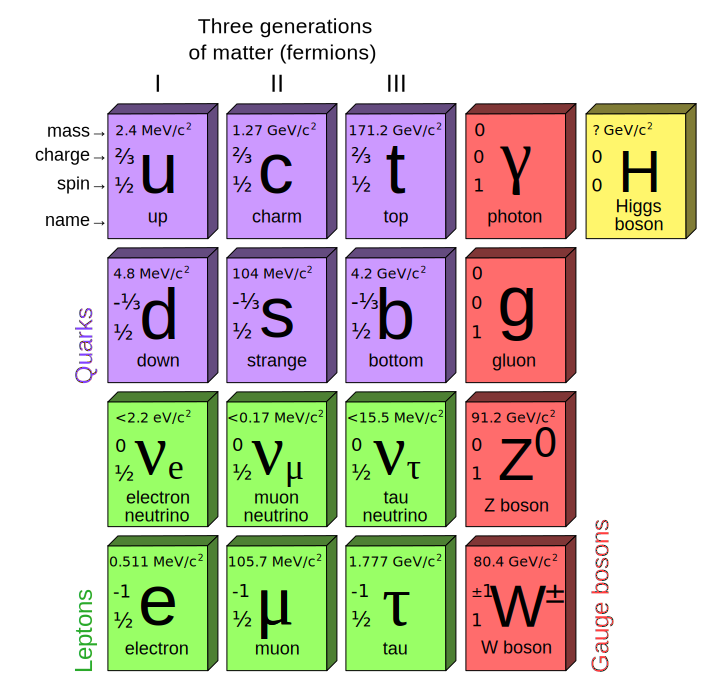
\includegraphics[scale=0.5, angle=0]{./figs/StandardModel}
    \caption{A table summarizing the particles described by the
    Standard Model of particle physics. The Standard Model encompasses
    three generations of quarks and leptons as well as four force carrying
    bosons.}
    \label{fig:sm}
\end{figure}

The Higgs boson is an essential component of the Standard Model and plays
an important role in the predictive power of the theory. Like much of modern
physics, the Standard Model relies heavily on the symmetries of nature. Just
as concepts such as conservation of momentum and energy can be tied to the 
fact that a system is symmetric under translations in space and time\footnote{
This result is known as Noether's Theorem and can be attributed to the 
brilliant German mathematician Emmy Noether.}, much of the mathematical 
framework of the Standard Model is based on internal symmetries 
known as gauge symmetries. In fact there are three gauge symmetries found
in the Standard Model\footnote{ In group theoretic language the symmetries of
the Standard Model can be written as $SU(3) \times SU(2) \times U(1)$.} 
each of which predicts a force carrying particle that mediates one of the 
aforementioned interactions of nature. The photon mediates the 
electromagnetic interaction. The massless gluon is responsible for the strong 
interaction, which binds quarks together to form protons and neutrons.
And finally, the weak interaction, which causes radioactive decays, 
is mediated by the massive \WBosons and \ZBoson bosons. The problem with all 
of this symmetry is that it predicts that the weak nuclear force is a long
range force, something which is not observed in nature. The reason for this
discrepancy can be traced back to the fact that the \WBoson and \ZBoson bosons are
not massless particles, but have a mass of roughly 80 and 90 GeV respectively. 
In addition, these internal gauge symmetries also predict that other 
fundamental particles, such as the electron, are massless. In order to solve
this apparent predicament one needs to introduce a mechanism that keeps the
equations that govern the Standard Model's behavior symmetric, but allows for
some asymmetric lowest energy states, i.e. 'ground states'. 
This is accomplished with a theoretical mechanism known as spontaneous
symmetry breaking or in this special case the Higgs mechanism.

On July 4th, 2012 the ATLAS and CMS collaborations both announced the 
discovery of a particle consistent with the 
Standard Model Higgs boson~\cite{ATLAS_Higgs,CMS_Higgs}, indicating that
the discovery of the mechanism behind spontaneous symmetry breaking in the
Standard Model may be at hand. In addition, the ATLAS experiment measured 
this Higgs-like boson's mass to be close to 125 GeV~\cite{ATLAS_Higgs_Dec12}.
This measurement is only the beginning of a challenging program of `Higgs
identification' through which the consistency of this new boson with the SM
Higgs will be verified or disproved. For this reason it is now becoming
increasingly important to measure the properties of this new scalar particle
as well as its rate of decay for the largest number of experimentally
viable decay channels. These analyses could result in tension with the SM
Higgs prediction, for instance the rate of one or more measured decay channels
may differ from the SM prediction. The simplest mechanism for such a scenario
is an enhancement/suppression in loop-induced decays
\footnote{A loop means that particles of any mass can instantly materialize and 
then disappear during the decay process. The brief-lived virtual particles
are usually $W$ bosons, but other particles with similar behavior can enter
the loop, including many beyond the Standard Model particles. This makes decays 
involving loops very sensitive to new physics at high masses.}
that are naturally sensitive to couplings to new virtual particles, 
for instance the decay \HToZg presented in this paper. 
This would thus be evidence for Beyond the Standard Model (BSM) physics.

The main decay modes being probed in the searches
presented on the July 4th announcement are the $H \to \gamma\gamma$ channel,
the $H \to WW^* \to 2\ell2\nu$ channel and the 'golden channel',
$H \to ZZ^* \to 4\ell$. However, little attention has been paid to the 
$H \to Z\gamma \to \ell^+\ell^-\gamma$ channel
despite the fact that its event rate is comparable to that of the golden channel 
for a 125 GeV Standard Model Higgs boson. The main reason for this is 
the low branching ratio for $Z \to \ell^+\ell^-$, the
probability that a $Z$ boson will decay into two leptons, 
makes the $Z\gamma$ channel statistically limited. 
Although, the background rate, the number of non-interesting physics processes
that contaminate the process of interest, of the $Z\gamma$ channel is higher than
that of the $ZZ^* \rightarrow 4\ell$ channel
there are a few important properties that make a study of the $Z\gamma$ channel 
compelling: 
1) all final state particles can be measured well with the ATLAS detector;  
2) the Higgs mass could be measured from the total invariant mass spectrum; 
3) the spin of the Higgs can be studied by analyzing the angular distribution 
of the decay products, and 
4) this channel can be used for setting limits on the Higgs coupling constants.
In addition, the ratio of $\gamma\gamma$ to $Z\gamma$ branching ratios can
be used to discriminate between certain models of 
new physics~\cite{Zg_newPhy_1,Zg_newPhy_2, Zg_newPhy_3}.
All of these measurements will help to identify this new particle sitting
close to 125 GeV as a Standard Model Higgs boson or something more exotic.

% re-write this with my own words....
This report documents the measurements of the \HToZg production rate observed
using data from $pp$ collisions provided by the LHC. In the following, the
theory behind the \HToZg decay is discussed in Section~\ref{sec:theory},
the ATLAS detector is described in Section~\ref{sec:atlas}, and the signal
and backgrond simulation samples used in the analysis are presented in
Section~\ref{sec:sigbkg}. The event selection criteria are described in 
Section~\ref{sec:event}. A comparison between the selected data sample and
the simulation is presented in Section~\ref{sec:compare}. The discrimination
between signal and background events is performed by means of an unbinned
maximum likelihood fit, and the estimated signal yield is compared to the one 
predicted by the Standard Model. The properties of the signal, in terms of
the expected yields and the signal model used for the fit are described
in Section~\ref{sec:signal}, while the choice of the background model adopted
in the fit is motivated in Section~\ref{sec:background}. After a description of
the systematic uncertainties in Section~\ref{sec:sys}, Section~\ref{sec:results}
presents the results of the combined analysis of the 7 and 8 TeV datasets.

\label{sec:intro}

\section{Theory}
\label{sec:theory}

This section is devoted to laying out a more formal description of the
theory presented in Section~\ref{sec:intro}. While the particles and
their properties tabulated in Figure~\ref{fig:sm} summarize the important
players in the study of elementary particles, an understanding of the
mathematical ideas behind the Standard Model's construction are essential in grasping
the importance of this measurement. This paper is focused on the measurement
of \HToZg at the LHC; therefore, a rigorous development of this ideas is forgone. 
For this see Halzen and Martin~\cite{QuarksLeptons}.

% Section~\ref{subsec:qed} gives a brief
% introduction to Gauge Theory and Quantum Field Theory through the simplest
% theory contained in the Standard Model: Quantum Electrodynamics (QED).
% Afterward the Higgs Mechanism is explained in Section~\ref{subsec:higgsmec}
% and finally the production processes studied in this measurement are
% given in Section~\ref{subsec:prodproc}.


\subsection{The Role of Symmetry in Particle Physics}
\label{subsec:symmetry}

An important principle motivating the mathematical structure of modern physical 
theories is the notion of symmetry. On a macroscopic scale one can study
the interactions of objects by holding them at various
distances apart and measuring the force between them. That is how Coulomb derived
the famous inverse square law describing electric repulsion and attraction that
now bears his name. On the smallest scales this empirical data is no longer
available, so that a new paradigm is need to understand how these interactions
come about. 

A beautiful solution was brought to light by the brilliant 
mathematician and physicist Emmy Noether who showed that every symmetry in
nature leads to a conserved quantity, a value that does not change over time.
A familiar application of this connection is found in Newton's third law:
For every action there is an equal and opposite reaction. From this balancing of
forces one can derive a conserved quantity associated with the system's 
motion, namely momentum. The importance of Noether's approach using symmetries
is that it allows the physicist to turn this reasoning around. One can postulate
the existence of a symmetry of nature, in this case the invariance of the laws
of physics under translations in space, which leads to a conserved quantity (momentum)
that results in experimentally testable predictions (Newton's third law).

While quantities such as momentum are familiar at the macroscopic level, 
it turns out that similar symmetries exist at subatomic distances
known as internal symmetries. One of the first examples of these symmetries
known as isospin was put forth by Werner Heisenberg in 1932 
to explain the approximate symmetry between
the newly discovered neutron with its partner in the atomic nucleus, the proton.
This symmetry says that according to the strong interaction that holds
the nucleus together the neutron and proton are reflections of each other,
i.e. the exchange proton $\leftrightarrow$ neutron does not affect the
physics of the strong force. More importantly this symmetry predicts that the
scattering rates of the interactions
\begin{align*}
    & p + p \rightarrow \pi^+ + d \\
    & \underbrace{p}_{\text{proton}} + \underbrace{n}_{\text{nuetron}} \rightarrow \underbrace{\pi^0}_{\text{pion}} + \underbrace{d}_{\text{deuteron}}
\end{align*}
should be equal. The experimental verification of this prediction convinced
physicists that these internal symmetries can be used to study and predict
how particles interact at the smallest length scales.

Physicists now use similar internal symmetries known as gauge symmetries to
describe the fundamental particles and their interactions. These gauge symmetries
are mathematical constructs similar to isospin that predict force carrying 
particles that mediate interactions in a way that can be used to calculate
various measurable quantities. The current gauge-theory formulation which describes
much of the phenomena found in nature is known as the Standard Model.

\subsection{The Standard Model}
\label{subsec:StandardModel}
A picture of the Standard Model of particle physics is best obtained
by moving away from the abstract gauge-theory formulation and instead considering
the predictive outcomes of the theory. The Standard Model provides physicists with
the current answer to the question of what the world is made of and is displayed
in Figure~\ref{fig:sm}. This table is reminiscent
of the periodic table developed by chemists to explain the various atoms
found in nature. Similar to the periodic table, the placement of particles in 
Figure~\ref{fig:sm} tells us something about the structure of these particles and
how they interact with each other. Some of these properties are labeled on
the figure including the particle's mass, charge, and 
spin\footnote{Spin is an internal quantum number of a particle which manifests 
itself as a particles intrinsic angular momentum.}.

\begin{figure}[htbp]
    \centering
    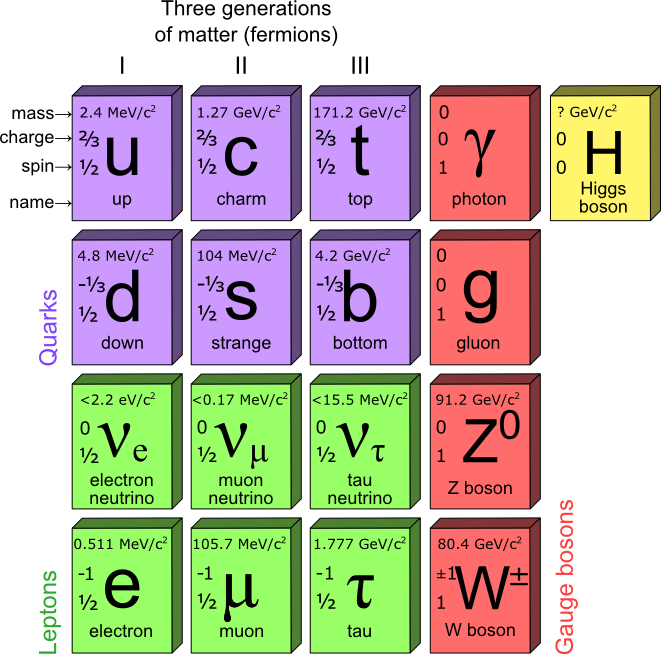
\includegraphics[scale=0.4, angle=0]{./figures/StandardModelPNG}
    \caption{A table summarizing the particles described by the
    Standard Model of particle physics. The Standard Model encompasses
    three generations of quarks and leptons as well as four force carrying
    bosons.}
    \label{fig:sm}
\end{figure}

A surprising property of the Standard Model is that it consists
of only 16 different particles. The first three columns consist of particles
that make up everyday matter known as fermions. A fermion is any particle that
has spin 1/2. 
For example, the first column contains two particles shown in purple known as
the up and down quarks, which are the building blocks of the familiar nucleons, 
i.e. the proton and the neutron. 
In addition, the second two particles marked in green
are the electron neutrino, which is produced abundantly in nuclear beta decay
($n \to p + e^- + \bar{\nu}_e$), as well as one of the most familiar fundamental
particles, the electron. In fact the atoms of the periodic table result when
the electron binds with the nucleons made of up and down quarks to form atoms. 
The Standard Model contains
three copies of this column structure composed of ever heavier particles.

The fundamental fermions are further divided into two types: quarks and leptons.
These forms of matter are separated by the various `charges' they carry. Quarks
(colored in purple in Figure~\ref{fig:sm})
carry both electric and color charge, so that they are the only particles that
interact via the strong force. 
On the other hand, leptons (colored in green in Figure~\ref{fig:sm}) 
do not carry color charge, so they do not interact with the strong force.
An important observation is that the ability of the quarks to interact via the
strong force allows them to overcome their electromagnetic repulsion and bind
together to form hadrons, particles composed of quarks. The proton and nuetron
are both examples of hadrons. Hadrons are further classified by the number
of constituent quarks that make them up. Baryons are made of three quarks while
mesons contain a quark and an anti-quark 
The proton, which is made of $uud$ quarks, is a baryon and
the $\pi^+$ is an example of a meson made up of $u\bar d$ quarks.
The various particle classifications used in particle physics are summarized in
\refF{fig:partclass}.

\begin{figure}[htbp]
    \centering
    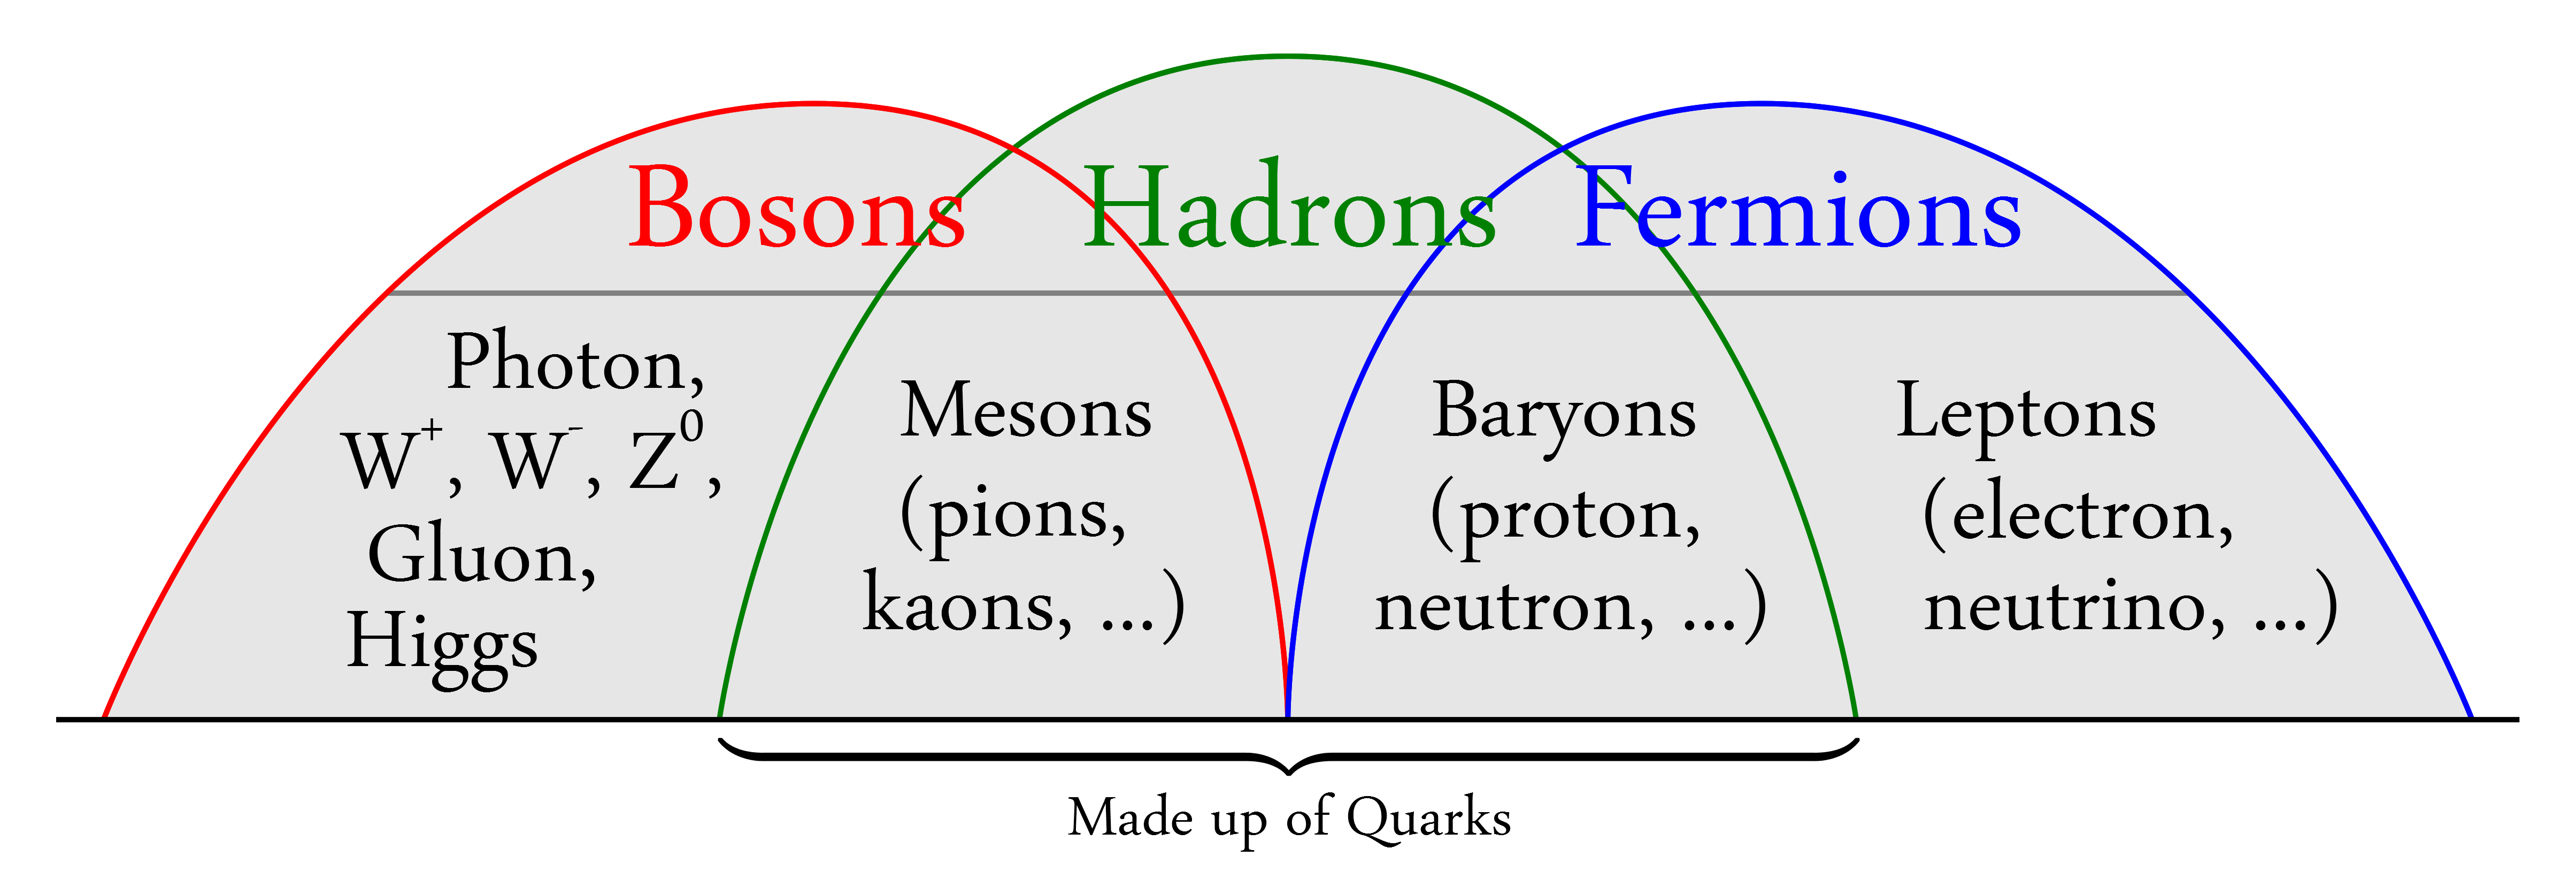
\includegraphics[scale=0.08, angle=0]{./figures/Bosons-Hadrons-Fermions}
    \caption{The different classifications of particles used in particle physics. Notice that hadrons are composed of both mesons and baryons, which are made up of quarks.
    The leptons are considered fermions because they have spin 1/2. The force carrying particles are bosons.}
    \label{fig:partclass}
\end{figure}

Finally there are four force carrying particles highlighted in red associated
with the gauge symmetries of the Standard Model. Mathematically, the gauge 
symmetry of the Standard Model is labeled as 
\[
\underbrace{\text{SU}(3)}_{\text{Strong Force}} \times \underbrace{\text{SU}(2) \times \text{U}(1)}_{\text{Electroweak Force}}.
\]
What this means is that each gauge symmetry is associated with particles.
These particles are known as gauge bosons and are responsible for mediating three 
out of the four fundamental forces in nature: the electromagnetic, strong, and 
weak interactions. As of now, theorists have been unable to incorporate the 
gravitational force, a pervasive component of the macroscopic world,
into the current gauge-theory of particle physics.
The SU(3) gauge symmetry describes the strong force, which
is mediated by the massless gluon. This force is responsible for binding
quarks together to form protons and neutrons. The weak interaction is
contained in the SU(2) gauge symmetry and is transmitted by the massive \WBosons
and \ZBoson bosons. The weak force is responsible for radioactive decays. The
last symmetry of the Standard Model, U(1), describes the familiar electromagnetic
interaction and is carried by the massless photon. The interaction of the force
carrying bosons with the Standard Model particles is graphically represented in 
\refF{fig:interactions}.

\begin{figure}[htbp]
    \centering
    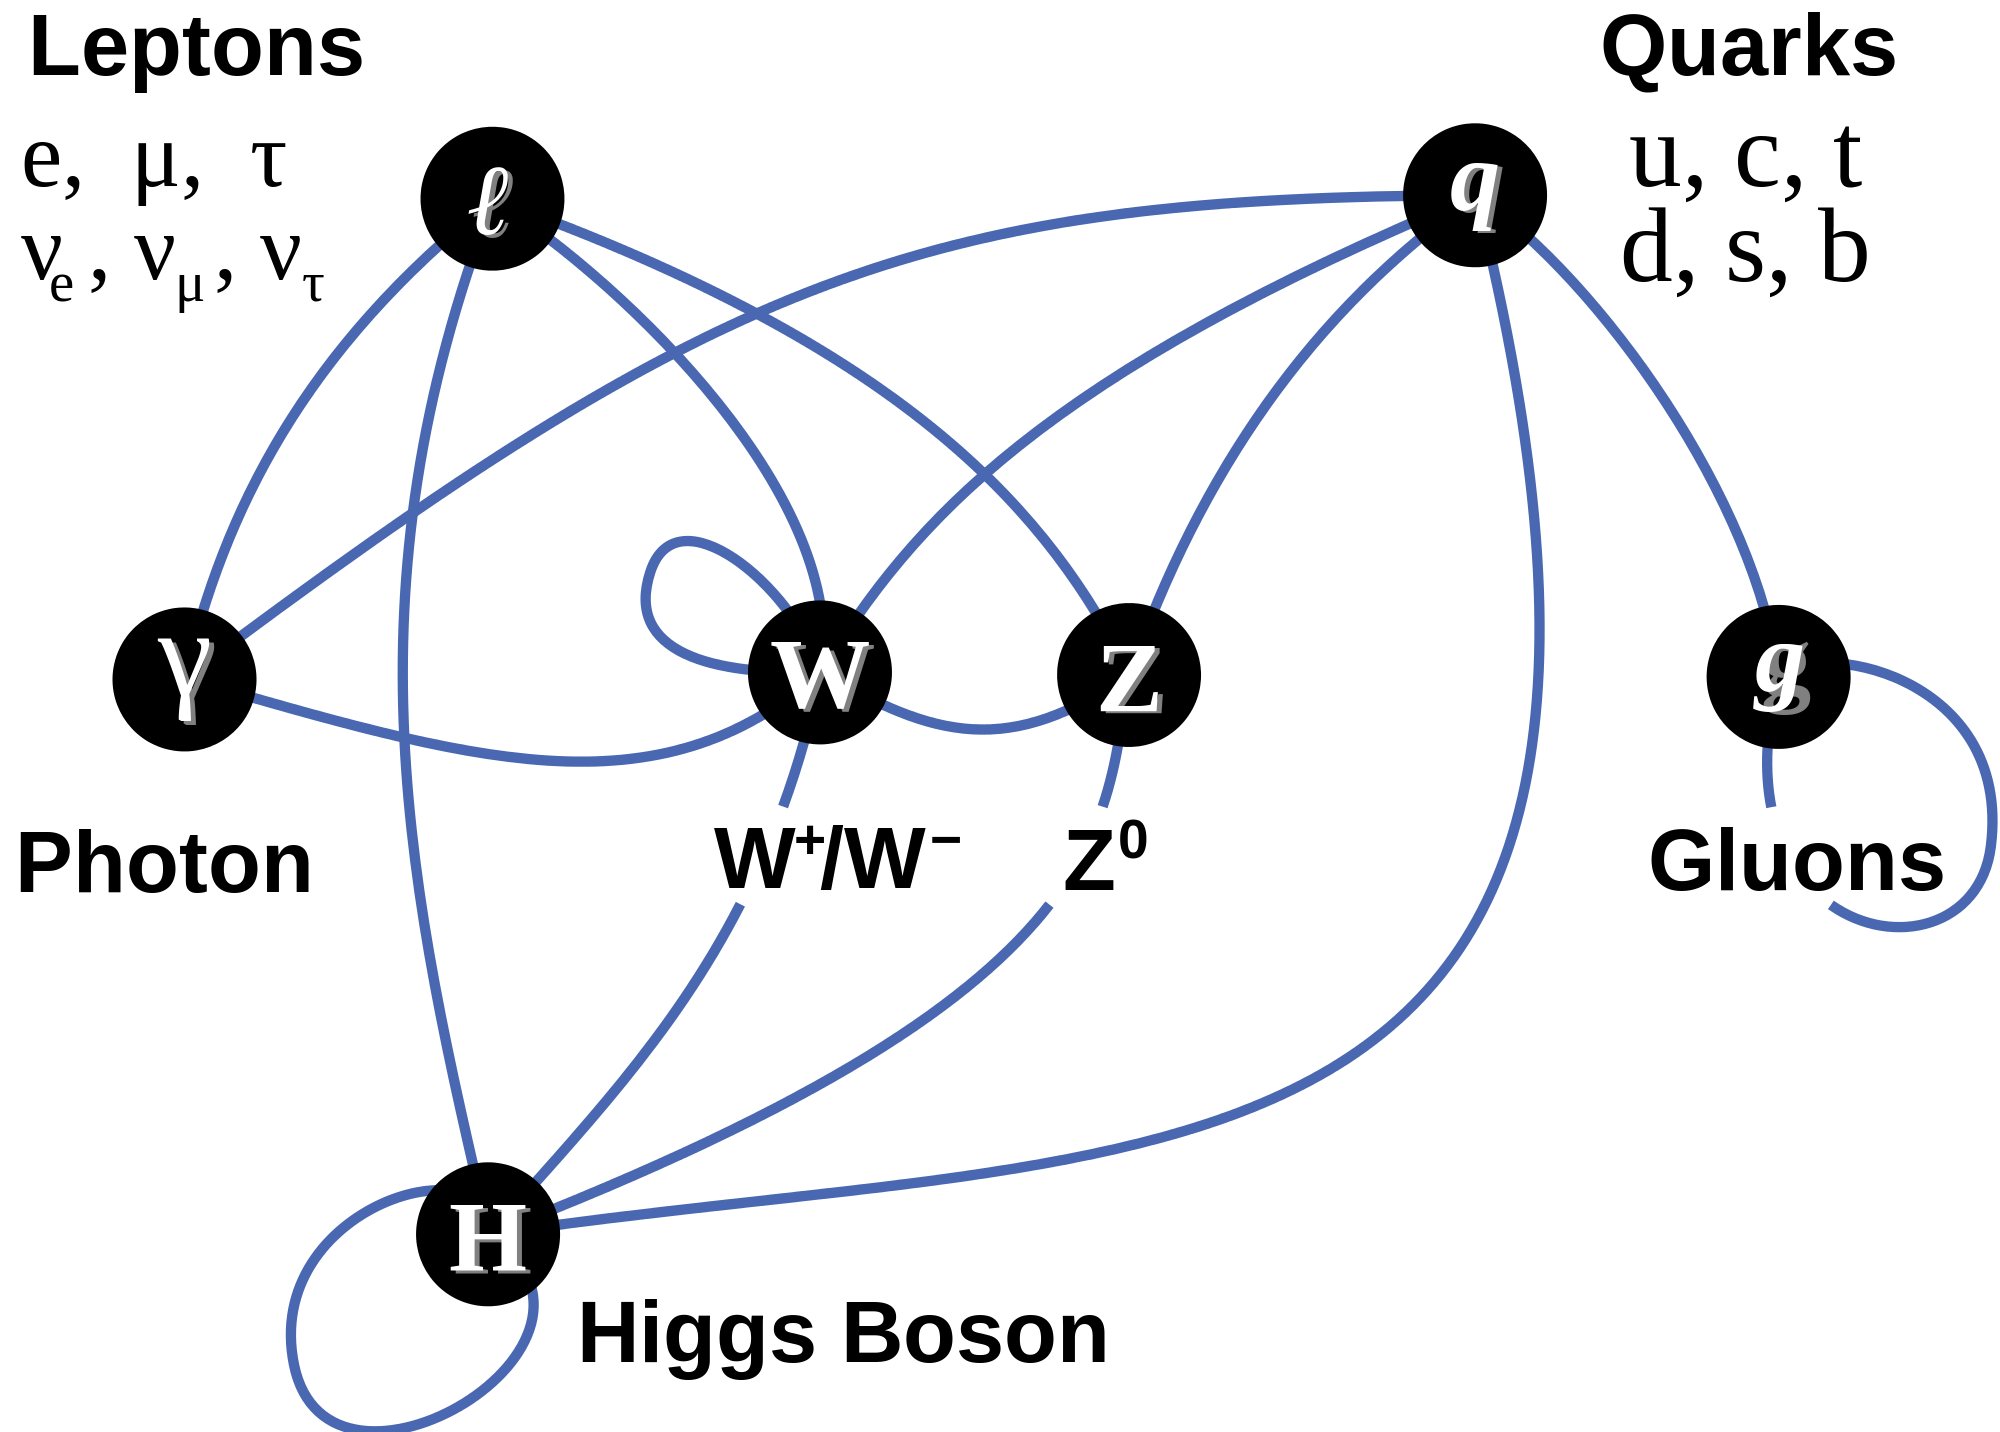
\includegraphics[scale=0.1, angle=0]{./figures/Elementary_particle_interactions}
    \caption{A graphical summary of the various interactions between particles 
    predicted by the Standard Model. 
    Notice that the leptons do not couple to the gluons, while
    the quarks couple to gluons as well as the electroweak force carriers.}
    \label{fig:interactions}
\end{figure}

The Standard Model together with Einstein's theory of gravity describes almost
all known phenomena from the largest scales to the smallest scales. Despite
its ability to precisely predict a large variety of experimental results, the
Standard Model does not account for the complete picture. Although not exhaustive
the following list contains a few inadequacies of the Standard Model:
1) It does not attempt to explain gravitation. As of yet a quantum theory of
gravity remains unknown.
2) The model contains 19 numerical constants whose values are not predicted
by the theory.
3) The Standard Model has no mechanism to explain the presence of the measured
missing mass and energy in the universe, the so called dark matter and dark energy 
problem. Despite these shortcomings, the gauge symmetries of the Standard Model 
remain a very powerful predictive tool responsible for explaining much of
what we know about the subatomic world.


\subsection{The Higgs Mechanism}
\label{subsec:higgsmec}
However, there is a problem with all of these gauge symmetries.
They predicts that the weak nuclear force is a long
range force, something which is not observed in nature. The reason for this
discrepancy can be traced back to the fact that the \WBoson and \ZBoson bosons are
not massless particles, but have a mass of roughly 80 and 90 GeV respectively. 
In addition, these internal gauge symmetries predict that other 
fundamental particles, such as the electron, are massless. In order to solve
this apparent predicament one needs to introduce a mechanism that keeps the
equations that govern the Standard Model's behavior symmetric, but allows for
some asymmetric lowest energy states, i.e. 'ground states'. 
This is accomplished by the Higgs mechanism, which combines two theoretical ideas
known as spontaneous symmetry breaking and local gauge invariance to give particles 
mass.

\subsection{Production Process}
\label{subsec:prodproc}

\begin{figure}[!htbp]
  \begin{center}
  {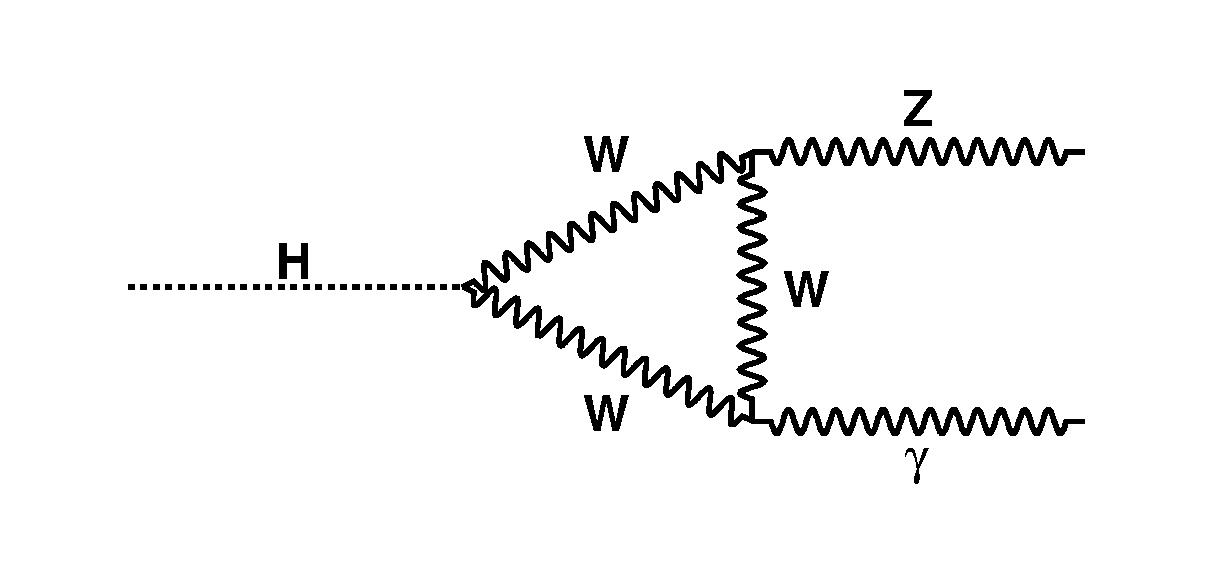
\includegraphics[width=2in]{figures/loop1}}
  {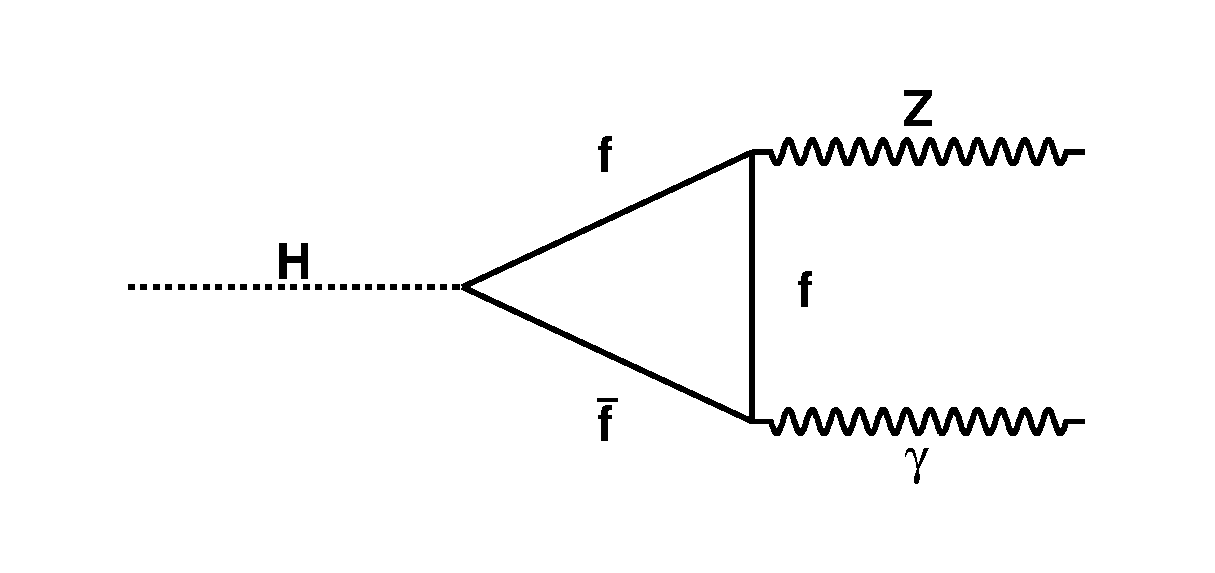
\includegraphics[width=2in]{figures/loop2}}
  {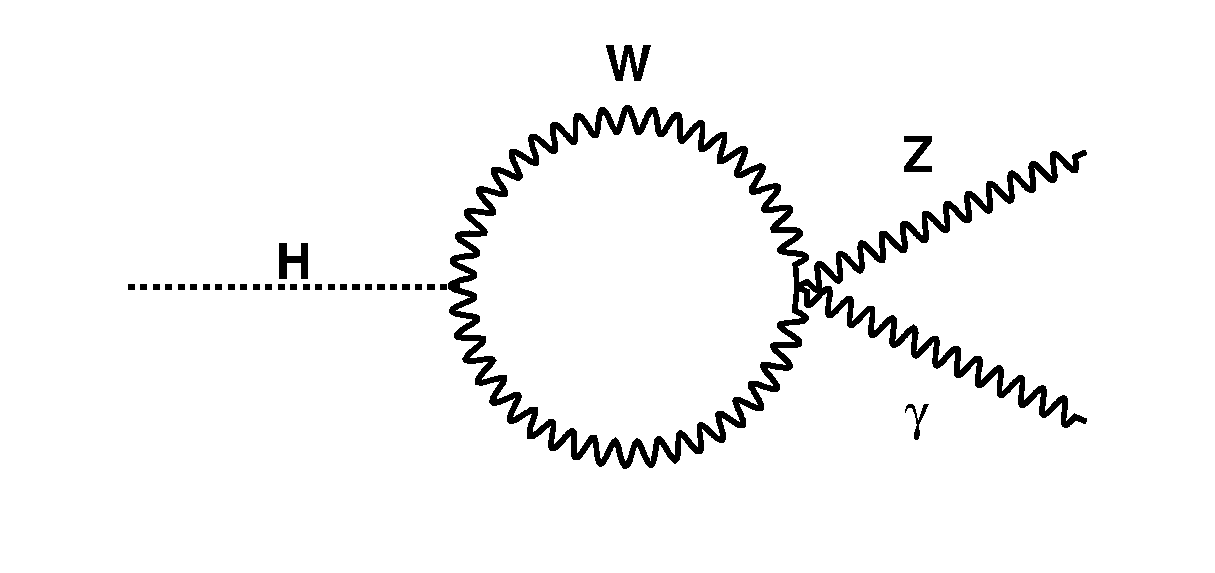
\includegraphics[width=2in]{figures/loop3}}
  \caption{Leading Feynman diagrams for the $H\rightarrow Z\gamma$
    decay in the Standard Model. Note that in the case of the fermion
    loop, top quarks dominate.} 
  \label{fig:feynman}
  \end{center}
\end{figure}


\section{Experimental Apparatus}
\label{sec:experiment}

As discussed in \refS{subsec:prodproc}, the detection of \HToZg events requires
colliding protons head on at very high energies in order to produce a shower
of particles whose kinematic properties must be subsequently measured.
The first step, obtaining proton-proton collisions at high center-of-mass energies,
is accomplished by the accelerator complex that makes up the Large Hadron Collider.
Subsequently, the ATLAS detector takes up the difficult task of measuring
the proceeding shower of hadrons and leptons necessary to find the Higgs boson
as well as any new physics.
\refS{subsec:lhc} describes the LHC accelerator
complex in detail and \refS{subsec:atlas} provides an overview of the various
particle detection apparatus that make up the ATLAS detector.

\subsection{The Large Hadron Collider}
\label{subsec:lhc}
The Large Hadron Collider (LHC) is the world's largest and highest-energy particle
accelerator. The LHC sits in a circular tunnel 27 km in circumference under
the Franco-Swiss border near Geneva, Switzerland. The LHC accelerates protons
to a velocity of 99.9999964\% the speed of light \cite{LHCdesign}. The full
complex of accelerators that dump protons into the LHC and other CERN 
experiments is displayed in \refF{fig:accelerator}.

\begin{figure}
  \centering
  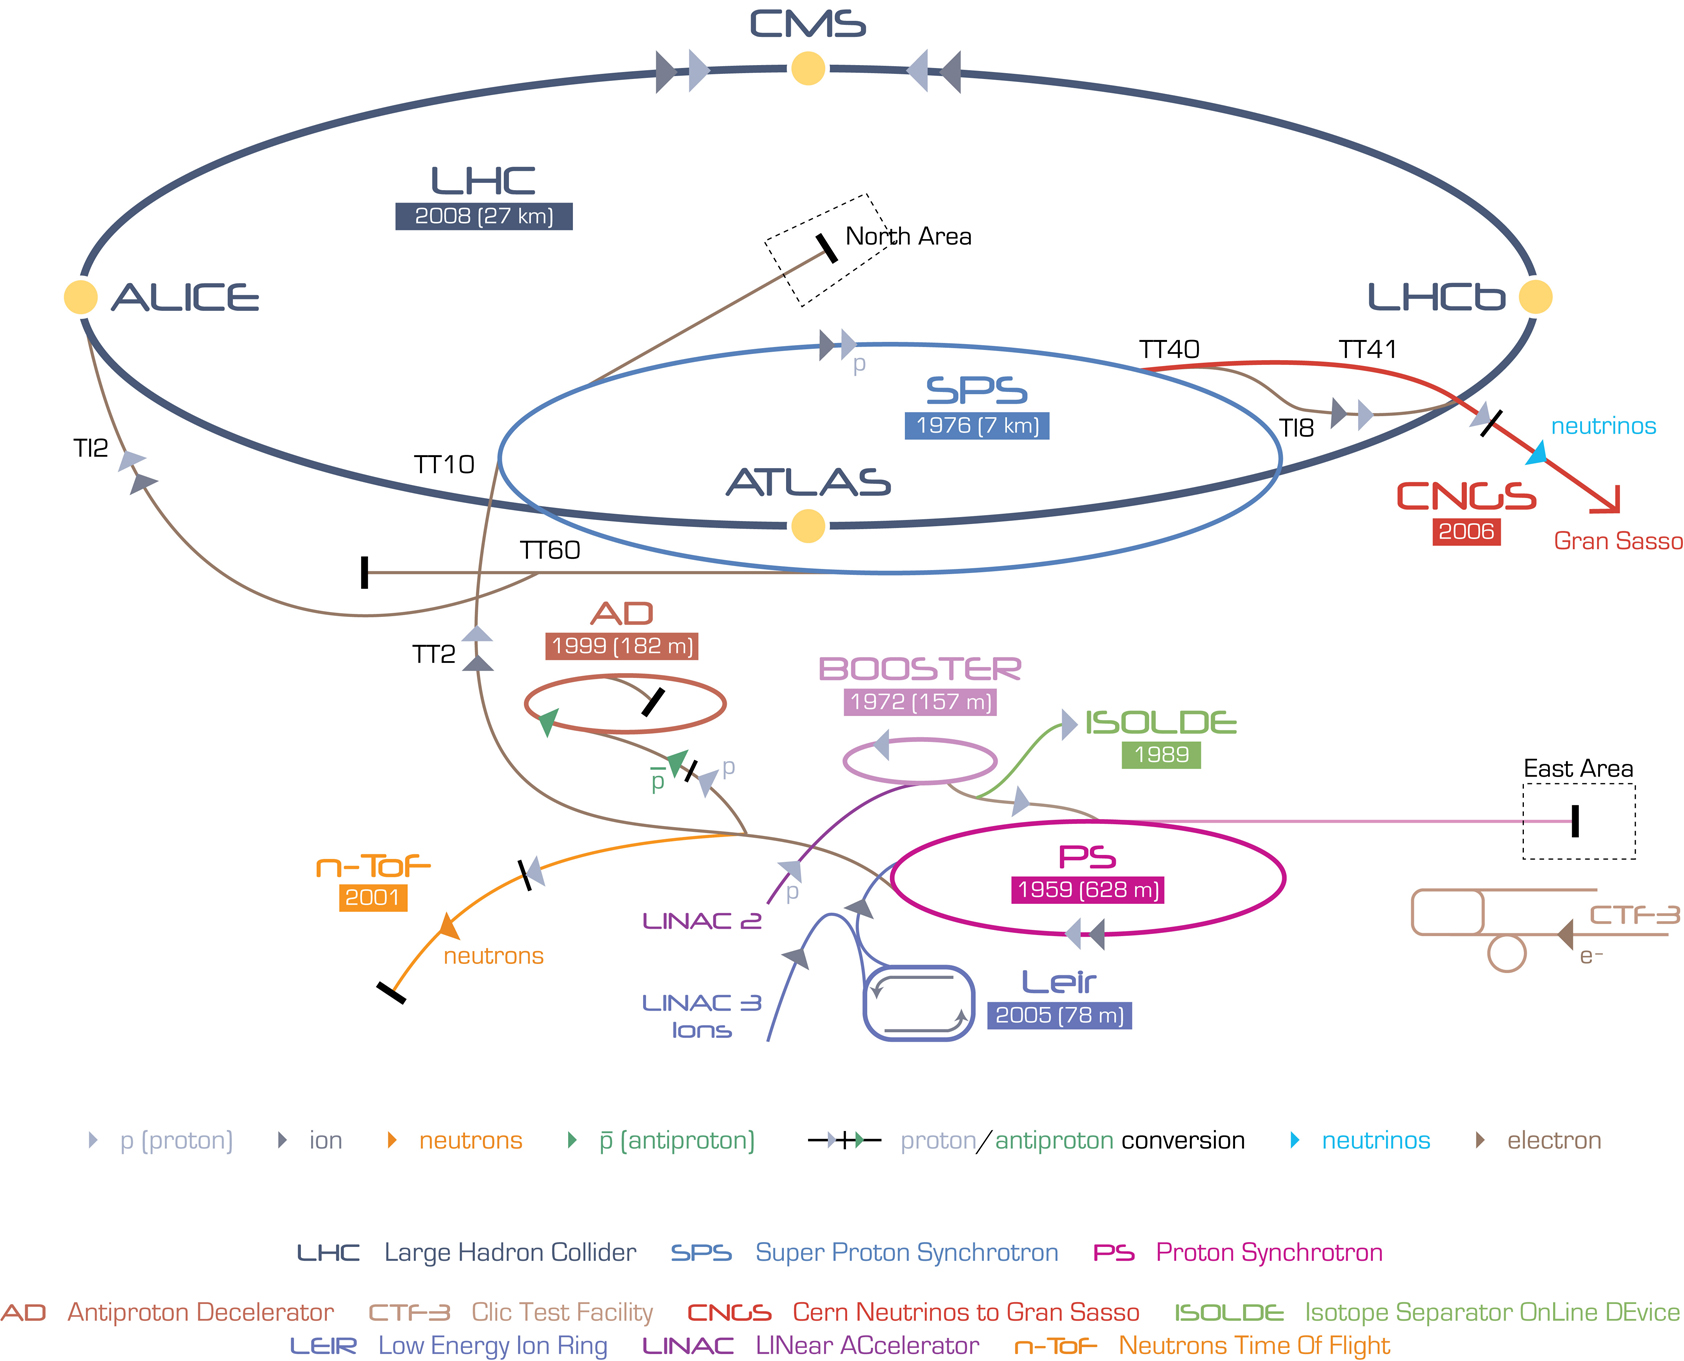
\includegraphics[scale=0.5, angle=0]{figures/Cern-Accelerator-Complex}
    \caption{The full complex of accelerators that dump protons into the LHC
    and other CERN experiments. Protons, which are stripped from hydrogen atoms,
    are accelerated to 99.9\% of the speed of light by passing through a series
    of accelerators: LINAC2, PSB, PS, SPS, and finally the LHC itself.}
  \label{fig:accelerator}
\end{figure}

Particle accelerator performance is characterize by two important quantities:
its center-of-mass energy and luminosity.
The center-of-mass energy of the colliding particles dictates what can
be produced in the collisions.
Larger values are necessary
to produce more massive particles because of conservation of energy and momentum. 
The LHC is designed to collide particles
at a center-of-mass energy of 7 TeV in 2011 and 8 TeV in 2012. This means
that each proton was accelerated to an energy of 3.5 and 4 TeV by the LHC
accelerator complex in 2011 and 2012 respectively. 
In addition to producing high energy collisions,
the LHC must also provide enough collisions to produce rare decay processes,
such as \HToZg.
The event rate $R$ for a physics process with a cross-section $\sigma$
is proportional to the collider's instantaneous luminosity $L$: $R = L\sigma$. 
The luminosity
is characterize by a few important properties of the accelerator:
\[
    L = \frac{k n^2 f}{4\pi \sigma_x \sigma_y}
\]
where $k$ is the number of proton bunches in the proton beam, 
$n$ is the number of protons per
bunch, $f$ is the revolution frequency, and $\sigma_x\sigma_y$ is the
beam size at the collision point. The value of these parameters at the
LHC are given in \refT{tab:lhcparameters}. In addition to being the most
energetic accelerator, the LHC also has the highest luminosity of any particle
collider with an instantaneous luminosity of roughly $10^{34}$ \cm{-2} \sec{-1}.

It should be noted that often what is of interest is not the instantaneous luminosity,
$L$, and the corresponding  event rate $R$, but rather the total number
of events produced of a physics process, i.e. $R \times ~\mathrm{time}$. Therefore,
one is interested in the integrated luminosity defined as 
$\mathcal{L} = \int L dt$, so that $N = \mathcal{L}\sigma$ where
$N$ is the number of events produced of a given process with cross-section $\sigma$.
The integrated luminosity used in this measurement was 4.5 (20.7) \fb in 2011 (2012).

\begin{table}[htbp]
  \begin{center}
    \begin{tabular}{cc}
    \hline\hline
    parameter & value  \\
    \hline
    $k$ &  $1.15 \times 10^{11}$ \\
    $n$ & 2808 \\
    $f$ & 11.25 Hz \\
    $\sigma_x\sigma_y$ &  16 $\mu$m\\
    \hline\hline
    \end{tabular}
    \caption{Parameters characterizing the LHC's luminosity. The integrated luminosity
    used in this measurement was 4.6 (20.7) \fb in 2011 (2012) \cite{LHCdesign}.}
    \label{tab:lhcparameters}
  \end{center}
\end{table}

The operation of the LHC is based on a series of accelerators that get the
proton bunches to the desired center-of-mass energy. Protons are obtained by
stripping hydrogen atoms of their single electron. These protons are then passed into
the LINear ACcelerator 2 or LINAC 2, which is the purple line in the bottom middle
of \refF{fig:accelerator}. The LINAC 2 accelerates these protons to an energy of
50 MeV, or 31.4\% of the speed of light. Then the protons are diverted into the
first circular accelerator, the Booster (denoted as BOOSTER
in Fig. \ref{fig:accelerator}). As well as accelerating protons up to 1.4 GeV,
the booster uses a sequence of quadrupole magnets to squeeze the bunches down 
so that they have a smaller cross-section. Aftward the protons are inserted
into the Proton Synchrotron (PS), which accelerates these protons to an energy
of 25 GeV at a velocity of 99.93\% the speed of light. The PS also uses 
radiofrequency pulses to chop the bunches into smaller sections, which can
be diverted to the various experiments around the CERN accelerator complex.
Then the PS Booster
injects the protons into the Super Proton Synchrotron (SPS) -- the 7 km light blue
ring in the figure. Here protons are accelerated to an energy of 450 GeV,
with a velocity of 99.9998\% the speed of light. These protons finally enter
the LHC ring, which increases the proton energy to 3.5 (4.0) TeV. The result
is a proton beam that collides at 7 (8) TeV in 2011 (2012).

There are six particle detectors located at the LHC designed
to identify the various particles produced during the collisions. TOTEM and LHCf
are designed to measure various scattering cross-sections, diffractive processes, 
and cosmic ray physics. The ALICE detector specializes in detecting the products
of heavy ion collisions in
order to study the quark-gluon plasma of the early universe. ATLAS and CMS 
are general purpose detectors designed to detect a large spectrum of particles
with a goal of finding signs of new physics. The measurement presented in this
paper uses data collected by the ATLAS detector.

\subsection{The ATLAS detector}
\label{subsec:atlas}

The ATLAS detector~\cite{Aad:2008zzm} is a multi-purpose particle physics detector
with approximate forward-backward symmetric cylindrical geometry. The detector
is 25 m in height, 44 m in length, and weights approximately 7000 tonnes. 
Since most particles of interest produced at the LHC are unstable
and decay before they can reach the detector, the ATLAS detector
was designed to detect and distinguish stable particles such as photons,
electrons, and protons. 
The kinematics of the unstable particles
are then calculated from the kinematics of their stable decay products
using conservation of energy and momentum.  In particular, the ATLAS
detector must be able to measure the
number of stable particles that result from the collision, the topology
of the event i.e. the particle's tracks\footnote{The trajectory of a charged
particle through the magnetic field of the detector is reffered to as a track.}, and 
the momentum, energy and identity of these particles.
A single detector cannot measure
all of these properties; therefore, the ATLAS detector consists of various
sub-detectors whose roles fall within two broad categories:
tracking detectors that measure the position of a charged particle with
minimal disturbance, and calorimeters that measure the energy of a particle
by total absorption. The ATLAS detector consists of
an inner tracking detector, an electromagnetic calorimeter, a hadronic calorimeter,
and a muon spectrometer. An artist's rendition of the ATLAS detector is 
displayed in \refF{fig:atlas}.
 
\begin{figure}[!hbpt]
  \centering
  \includegraphics[scale=0.5, angle=0]{figures/atlas}
  \caption{Cut-away view of the ATLAS detector. The dimensions of the detector
  are 25 m in height and 44 m in length. The overall weight of the detector
  is approximately 7000 tonnes.}
  \label{fig:atlas}
\end{figure}

The inner tracking detector (ID) lies closest to the beam pipe and reconstructs
the path of charged particles with the information provided by a 2 T solenoidal
magnetic field. In addition, the inner detector provides momentum
and decay vertex measurements and electron identification. A more in depth
description of the inner tracking system is provided in \refS{subsubsec:id}.
The electromagnetic calorimeter (EM calorimeter) surrounds the inner detector
and measures the energy of light particles that interact electromagnetically such 
as electrons and photons. The hadronic calorimeter encircles the EM calorimeter
and is responsible for measuring the energy of composite hadrons such as protons
and neutrons. The operating principles as well as the geometric details of
the calorimeter system are presented in \refS{subsubsec:calo}. The calorimeter
is surrounded by the muon spectrometer. The muon spectrometer measures the tracks
of the charged muons, which are massive enough to pass through the inner parts
of the detector. The muon spectrometer is described in \refS{subsubsec:muonspec}.

A more complete description of ATLAS splits the detector
into a barrel part, where the detector layers
are positioned on cylindrical surfaces around the beam axis, and two end-cap parts,
where the detector layers are positioned in planes of constant $z$ perpendicular
to the beam pipe. In addition, the calorimeter consists of a forward 
and backward part, extending up to a pseudorapidity\footnote{For a description
of the coordinate system employed at ATLAS see \refS{subsubsec:kinematics}.} 
of $|\eta| < 4.9$. The dimensions of the various components of the ATLAS detector
are displayed in \refT{tab:atlasdim}.

\begin{table}[htbp]
  \begin{center}
    \begin{tabular}{|l|ccc|}
    \hline
    Component & radius [m] & length [m] & $\eta$ coverage \\
    \hline
    barrel muon spectrometer &  11 & 26 & $|\eta| < 1.4$ \\
    end-cap muon spectrometer & 11 & 2.8 & $1.1 < |\eta| < 2.8$ \\
    \hline
    barrel hadronic calorimeter & 4.25 & 12.2 & $|\eta| < 1.0$ \\
    end-cap hadronic calorimeter & 2.25 & 2.25 & $1.5 < |\eta| < 3.2$ \\
    \hline
    barrel em-calorimeter & 2.25 & 6.42 & $|\eta| < 1.4$ \\
    end-cap em-calorimeter & 2.25 & 0.63 & $1.4 < |\eta| < 3.2$ \\
    forward/backward calorimeter & N/A & N/A & $3.1 < |\eta| < 4.9$ \\
    \hline
    barrel + end-cap inner detector & 1.15 & 6.8 & $|\eta| < 2.5$ \\
    \hline
    \end{tabular}
    \caption{Dimensions of the ATLAS sub-detectors.}
    \label{tab:atlasdim}
  \end{center}
\end{table}

\subsubsection{Kinematic quantities at ATLAS}
\label{subsubsec:kinematics}

The geometry of the ATLAS detector is defined
by a right-handed coordinate system with its origin at the point of
the proton-proton collision (PC) located at the center of the detector 
and the $z$-axis along the beam pipe. 
The $x$-axis points from the PC to the center of the LHC 
ring, and the $y$-axis points upward. The $x$ and $y$ axes define
a plane perpendicular to the beam axis known as the transverse plane with
its origin on the beam pipe.

In addition to the rectangular coordinate system previously described,
cylindrical coordinates ($r, \phi$) are
used in the transverse plane, $\phi$ being the azimuthal angle around the
beam pipe. The full 3D geometry is then defined if a third coordinate is specified.
A quantity known as the pseudorapidty is used as the third coordinate, 
which is defined in terms of the 
polar angle $\theta$ as $\eta = -\ln \tan(\theta/2)$, e.g $\theta = 45\degr$
corresponds to $|\eta| = 0.9$. The reason for the use of $\eta$ as opposed
the $\theta$ is because $\eta$ is invariant with respect to longitudinal boosts. This
is important because in hadron collisions one is actually colliding the
constituent quarks and gluons, so that the net longitudinal momentum of the two
colliding partons will vary from collision to collision. Therefore, the laboratory
frame and the parton center of mass frame do not coincide. Instead the parton
center of mass frame is boosted along the beam axis. Thus a distribution
uniform in $\theta$ in the center of mass frame of the partons will not
be uniform in the laboratory frame. However, because $\eta$ is invariant
under longitudinal boosts these two distributions will coincide if $\eta$
is chosen as the third coordinate.

A few other quantities of interest that are invariant under longitudinal boosts
are a particle's transverse momentum $p_T$ and the separation in $\eta-\phi$
space deemed $\Delta R$. The transverse momentum $p_T$ is defined as the 
amount of a particle's momentum that is located in the plane perpendicular 
to the beam pipe (the $x$-$y$ plane). The distance $\Delta R$ 
is defined as $\Delta R = \sqrt{(\Delta \eta)^2 + (\Delta \phi)^2}$.

A kinematic observable that is very effective at discovering particle's at
ATLAS is known as the invariant mass. Consider the Higgs decay process
searched for in this paper: \HTollg where the $Z$ decays into two leptons.
The dilepton invariant mass $m_{\ell\ell}$ is
\[
    m^2_{\ell\ell} = (p_1 + p_2)^2
\]
where $p_1$ and $p_2$ are the four-momenta of the leptons $\ell^+$ and $\ell^-$.
Then
\[
    m_{\ell\ell} = \sqrt{(p_1 + p_2)^2} = \sqrt{(E_1 + E_2)^2 - (\mathbf{p_1} + \mathbf{p_2})^2}.
\]
The relationship of $m_{\ell\ell}$ with the mass $m_Z$ of the Z boson is that a
distribution of $m_{\ell\ell}$ will peak at $m_{Z}$. The concept of invariant
mass can be generalized to a multi-body system such as \HTollg as follows:
\[
    m_{\ell\ell\gamma} = \sqrt{(p_{\ell_1} + p_{\ell_2} + p_{\gamma})^2} =
    \sqrt{(E_{\ell_1} + E_{\ell_2} + E_{\gamma})^2 - (\mathbf{p}_{\ell_1} + 
    \mathbf{p}_{\ell_2} + \mathbf{p}_{\gamma})^2}. 
\]
The distributions of $m_{\ell\ell\gamma}$ and $m_{\ell\ell}$ are the primary
observables used to search for the Higgs boson in this analysis.

\subsubsection{Particle identification at ATLAS}
\label{subsubsec:particleid}
The ATLAS detector is designed so that the various particles produced in
proton-proton collisions leave different signatures in the detector. This
allows for a way to easily distinguish between the particles.
The interactions
of the different particle types with the detector are displayed in 
\refF{fig:particleid}. Photons are uncharged and leave no track in
the inner detector. Therefore, photons are characterized by large energy 
deposits in the electromagnetic calorimeter. Electrons are light charged particles
that interact with the tracking system and deposit their energy into the 
EM calorimeter. Just like the electron, hadrons such as protons and pions 
are charged particles that interact with the inner detector; however, their
large mass causes them to penetrate further into the detector and deposit
their energy into the hadronic calorimeter. Composite neutral particles
like the neutron do not interact with the inner detector; however, they
are detected by the electromagnetic and hadronic calorimeters. Muons
pass through the whole detector and are charged. Thus, they will leave a
track in both the inner detector and the muon spectrometer. Finally,
massless neutrinos which interact only through weak interactions
pass through ATLAS undetected
and are inferred through conservation of energy and momentum.

\begin{figure}[!hbpt]
  \centering
  \includegraphics[scale=0.4, angle=0]{figures/particle-tracks}
 % \begin{subfigure}[b]{0.45\textwidth}
 % \centering
 %     \includegraphics[scale=0.4, angle=0]{figures/particle-signatures}
 %     \caption{}
 %     \label{fig:particleenergy}
 % \end{subfigure}
  \caption{The components the make up the ATLAS detector. Each particle type
  has its own signature in the detector. For example, a particle that is
  only detected in the electromagnetic calorimeter is likely to be a photon.
  }
  \label{fig:particleid}
\end{figure}



% Before delving into the specifics of each component of the ATLAS detector,
% a brief overview of the physical processes responsible for particle detection
% is necessary. Particles are detected through their interactions with matter. As
% such the way in which particles are detected can be broken up into two categories:
% charged and uncharged particle detection. The main processes that lead
% to the detection of charged particles are energy loss through ionization, 
% bremsstrahlung, and hadronic interactions. The process of ionization 
% occurs when charged particles traverse a material and lose energy through
% collisions with atomic electrons, leaving these electrons free from the atom,
% i.e. ionized. This deceleration then leads to emission of a show of photons
% known as bremsstrahlung. The combination of ionization and bremsstrahlung
% is behind the basic operation of the electromagnetic calorimeter.

\subsubsection{The inner detector}
\label{subsubsec:id}
The inner detector surrounds the beam pipe and provides track reconstruction,
momentum information, and both primary and secondary vertex measurements for
charged tracks above a nominal $p_{T}$ threshold of 0.5 GeV and within
a pseudorapidity range of $|\eta| < 2.5$ ($\theta < 10^o$). ATLAS's ID also provides electron
identification over $|\eta| < 2.0$ and 
a range of energies between 0.5 GeV and 150 GeV. The basic
operating principle of the inner detector is to track charged particles
via the ionization of the medium in such a way that the particles lose very
little energy. 

An important ability of the inner detector is to provide a measurement of
a particle's momentum and charge. The whole inner detector is immersed in a 2 T
magnetic field produced by a solenoidal superconducting magnet that radially
surrounds the whole inner detector. The magnetic field produced by the
solenoid is parallel to the beamline, while the particle trajectories are
approximately radial. This means that $\mathbf{v} \times \mathbf{B}$ is proportional
to $\mathbf{\hat r} \times \mathbf{\hat z} = -\mathbf{\hat \phi}$ and
charged particles are deflected tangentially
\footnote{Recall the magnetic
component of the Lorentz force is $\mathbf{F} = q(\mathbf{v} \times \mathbf{B}$).}.
Using hits in all three sub-detectors, a
track of the flight path of a charged particle can be reconstructed. The
curvature of the track is then used to determine the particle's
momentum with the familiar relationship $|p| = \frac{q B}{R}$
where $q$ is the particles charge, $B$ is the strength of the magnetic field, and 
$R$ is the radius of the particle's track. The required momentum resolution
in the inner detector is $\sigma_{p_T}/p_T = 0.05\% p_T \bigoplus 1\%$
\cite{Innerdesign}.

\begin{figure}[!hbpt]
  \centering
  \begin{subfigure}[b]{0.45\textwidth}
      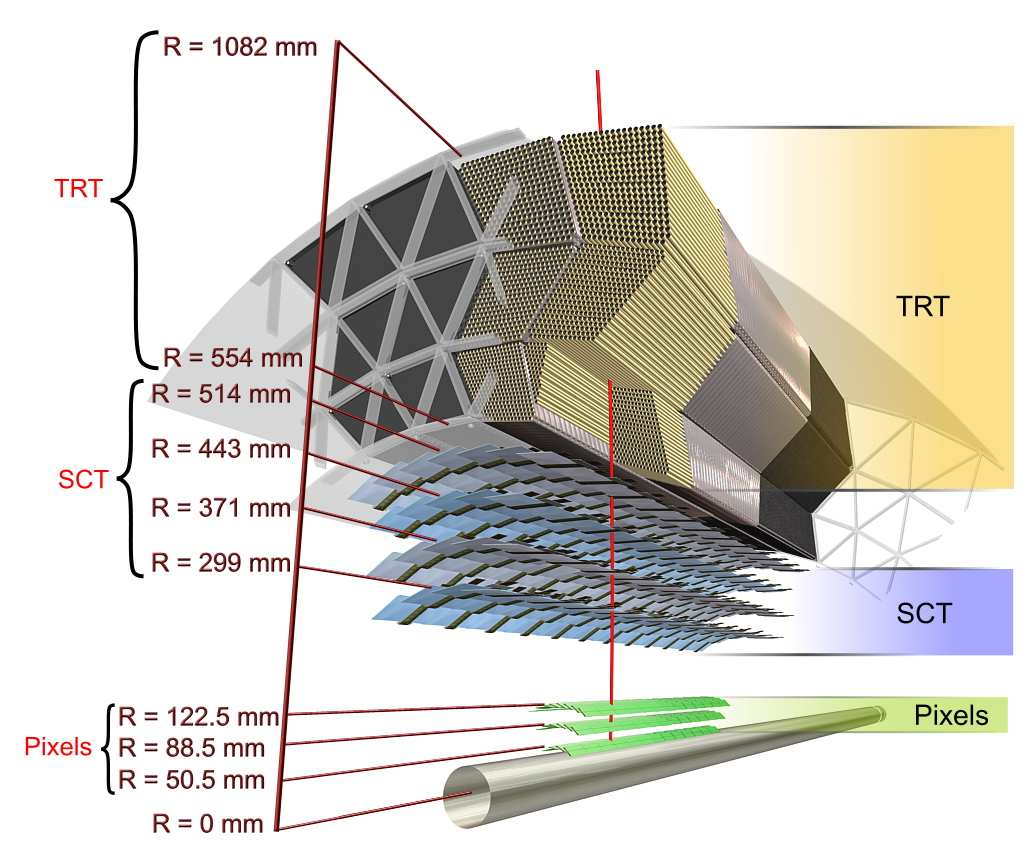
\includegraphics[scale=0.5, angle=0]{figures/id_perspective_layout}
      \caption{}
      \label{fig:idperspective}
  \end{subfigure}
  \quad
  \begin{subfigure}[b]{0.45\textwidth}
  \centering
    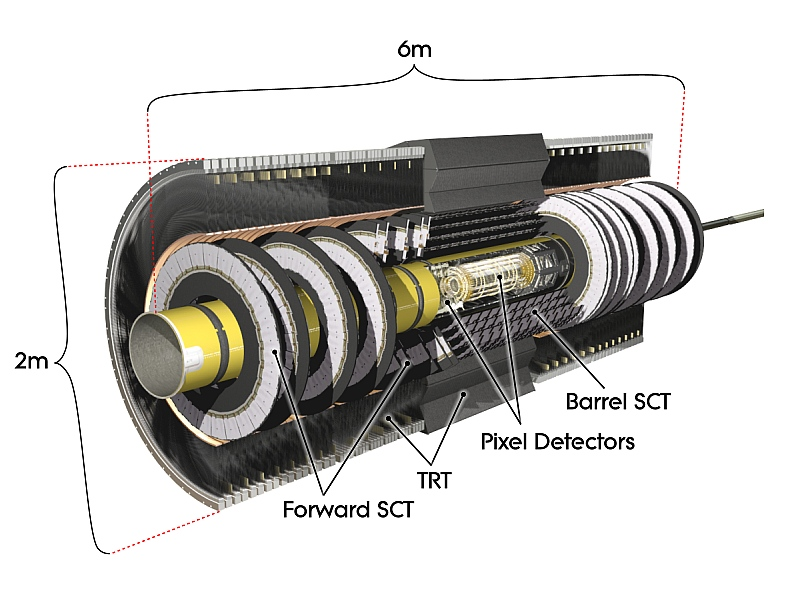
\includegraphics[scale=0.3, angle=0]{figures/Inner_detector}
    \caption{}
    \label{fig:id}
  \end{subfigure}
  \caption{Left-side:
  a cross-sectional view of the inner detector displaying the three tracking
  systems that make it up. Right-side: A complete three-dimensional view
  of the ATLAS inner detector.}
  \label{fig:innerdetector}
\end{figure}

The inner detector is comprised of three tracking systems: pixels,
the silicon central tracker (SCT), and the transition radiation tracker (TRT).
The configuration of these three trackers is displayed in \refF{fig:innerdetector}.
The three trackers operate independently from one another, but the information
is combined to form a complete track of a particle as it makes its way
through the inner detector. The spatial resolution and coverage of the inner detector
sub-systems is displayed in \refT{tab:spaceres}.

\begin{table}[htbp]
  \begin{center}
    \caption{Spatial resolutions and $\eta$-coverage of the sub-detectors
    that make up the ATLAS inner detector \cite{Aad:2008zzm}.}
    \label{tab:spaceres}
    \begin{tabular}{|ll|cc|}
    \hline
    Sub-Detector & Position & Resolution [$\mu$m] & $\eta$ Coverage \\
    \hline
    \textbf{Pixel} & 1 removable barrel layer & $R\phi = 10$, $z = 115$ & $\pm 2.5$ \\
     & 2 barrel layers & $R\phi = 10$, $z = 115$ & $\pm1.7$ \\
     & 4 end-cap disks on each side & $R\phi = 10$, $R = 115$ & 1.7-2.5 \\
    \hline
    \textbf{SCT} & 4 barrel layers & $R\phi = 17$, $z = 580$ &  $\pm 1.4$ \\
     & 9 end-cap wheels on each side & $R\phi = 17$, $z = 580$  & 1.4 - 2.5 \\
    \hline
    \textbf{TRT} & Axial barrel straws & 130 & $\pm 0.7$ \\
     & Radial end-cap straws & 130 & 0.7 - 2.5 \\
    \hline
    \end{tabular}
  \end{center}
\end{table}

\subsubsection*{The pixel detector}
The pixel detector, which sits as close to the interaction point as possible,
provides high precision measurements of a particle's track. The system
consists of 80 million pixels,
each of which is $50 \times 400\mu\mathrm{m}^2$ in dimension. Each charged
particle track transverses three pixel layers, which provides three precision
measurements. The system consists of three barrels at average radii of roughly
5 cm, 9 cm, and 12 cm, 
as well as three disks on each side, between radii of 9 and 15 cm.
The thickness of each layer is about 2.5\% of a radiation length of
nominal incidence.

The millions of pixels that comprise the pixel detector are made of
doped silicon, which acts as a diode when properly biased. These
pixels have a voltage across them to produce a wide depletion region across
the existing p-n junction. This large reverse bias means that no current
will flow through the electronics unless the diode breaks down. However,
when charged particles traverse the bulk silicon, they produce electron-hole pairs
through ionization of the semi-conductor's atoms. This current is then readout
and used to precisely locate the position of the particle. The resolution of
the pixel detector in the $R-\phi$ and $z$ directions 
are displayed in \refT{tab:spaceres}. Note that the resolutions
quoted are typical values and the actual resolution depends on $|\eta|$.

An important 
ability of the pixel detector is to determine the resolution associated with
the measurement of the impact parameter associated with secondary vertices
(decay vertices that occur right after the initial proton-proton collision). 
The minimum distance from the primary vertex to the secondary vertex is called
the impact parameter and it can be broken up into a component in the transverse
plane ($d_0$) and another component along the $z$-axis ($z_0$). A high resolution
of the impact parameter enables identification of secondary vertices
associated with very short-lived particles such as 
b-quarks and $\tau$-leptons. This allows for
better signal to background resolution for important process such as
$H \to b\bar b$ and $t \to W b$. In terms of
the polar angle $\theta$ and the particle's transverse momentum, 
The resolution for $d_o$ is
$\sigma(d_o) = 11 \bigoplus 60/p_T \sqrt{sin\theta}$ and the resolution in $z_o$
is $\sigma(z_o) = 70 \bigoplus 100/p_T \sqrt{sin^3\theta}$ in $\mu$m 
\cite{Aad:2008zzm}.

\subsubsection*{The semiconductor tracker}
At an intermediate radial range the Semiconductor Tracker (SCT) system contributes
to the measurement of momentum, impact parameter, and vertex position.
The SCT operates on the same principles as the pixel
detector; however, narrow strips of silicon $6.36 \times 6.40 \, \text{cm}^2$
in area are used instead of more precise silicon pixels. 
This allows measurement of only one coordinate (either $\phi$ or $z$), so the
SCT uses two orthogonally oriented strips glued back to back to measure both
$\phi$ and $z$. The four barrel layers are located at radii of roughly 3 cm,
3.71 cm, 4.43 cm, and 5.14 cm. This allows for four precision measurements of
a track's $R$, $\phi$, and $z$ coordinates. 
The spatial resolution of the SCT system is documented in \refT{tab:spaceres}.
Two tracks can be distinguished if they are separated by more than 200 $\mu$m.

\subsubsection*{The transition radiation tracker}
The transition radiation tracker (TRT) surrounds both the pixel and SCT detectors.
The TRT is a straw tracker made of roughly 60 layers of 
Polymide drift tubes (straws) of 4 mm diameter and filled with a combination
of Xenon, CO$_2$, and O$_2$ gas. 
The barrel contains about 50000 straws, and the end-caps contain 320000 radial straws.
When a charged particle transverses the drift tubes, the gas is ionized within
the straw. A voltage is applied to the wall of the straw and the central wire in
such a way that the negative free electrons resulting from the ionized gas
will drift to the central wire. The electron's drift velocity is known. Therfore,
the distance from the center of the straw to the flight path of the charged
particle can be determined using the timing between the arrival of the first
and last ionized electron. This process is outlined in \refF{fig:trt}. The
TRT only measures the position of a particle in the $\phi$ direction with
a resolution of 130 $\mu$m.

\begin{figure}[!hbpt]
  \centering
  \includegraphics[scale=0.4, angle=0]{figures/trtschematic}
  \caption{Cross-section of a bundle of TRT straw tubes.}
  \label{fig:trt}
\end{figure}

As well as providing spatial tracking, the TRT is designed to identify
electrons. The space between the straws is filled with a foam that has
a different index of refraction than the Xenon gas within the straws. When
ultra-relativistic particles\footnote{Particles with $\gamma = (1 - \beta^2)^{\frac{1}{2}} \approx 2000$.} cross the boundaries of these materials, they produce
transition radiation. This additional radiation will produce a high threshold
signature in the straw. Along with the energy measurement provided by the
calorimeter system, the presence of transition radiation can help identify
the particle as an electron (via $E = \gamma m c^2$).
 
% \begin{figure}[!hbpt]
%   \centering
%   \includegraphics[scale=0.4, angle=0]{figures/impactparameter}
%   \caption{Cross-section of a bundle of TRT straw tubes.}
%   \label{fig:trt}
% \end{figure}

\subsubsection{The calorimeter}
\label{subsubsec:calo}
The ATLAS calorimeter system is placed between the inner detector and the muon
spectrometer. The primary purpose of the calorimeters is to measure the energy
of both charged and neutral particles such as electrons, photons, and jets, 
and to determine the missing transverse energy. 
In addition, the calorimeters provide crude position measurements
as well as particle identification.

Calorimetry operates through the measurement of an incident particle's energy
by total absorption, where a fraction of the total energy is transformed
into a measurably quantity, i.e. charge or light. In practice,
each calorimeter is composed of metal sheets known as absorbers sandwiched 
between a detection medium. Particles interact with the absorbers transforming
the incident energy into a `shower' of secondary particles that are detected
in the detection medium. In a crude sense, the total number of particles
produced in these showers is proportional to the energy of the incident particle.
Thus, a calorimeter is a device designed to count secondary particles 
produced in these interactions.

\begin{figure}[!hbpt]
  \centering
  \includegraphics[scale=0.5, angle=0]{figures/calorimeter}
  \caption{Cut-away view of the ATLAS calorimeter system.}
  \label{fig:cal}
\end{figure}

The calorimeter system covers the range $|\eta| < 4.9$ and is composed of an
electromagnetic and hadronic calorimeter. The EM calorimeter is designed for
precision measurements of electrons and photons, while the hadronic calorimeter is
responsible for providing accurate measurements of jet energy and the reconstruction
of missing transverse energy $\slashed{E}_T$. The calorimeter was also designed
to contain the electromagnetic and hadronic showers so that they do not
make it through to the muon systems. Thus, the total thickness of the EM 
calorimeter is $> 22$ radiation lengths ($X_0$) in the barrel and $> 24\,X_0$
in the end-caps.
An overview of the ATLAS calorimeter system is displayed in \refF{fig:cal}.

\subsubsection*{Electromagnetic calorimeter}
The EM calorimeter consists of lead absorbers and liquid argon (lAr) sensing
elements, which provide optimized energy and position resolution for electrons
and photons within a pseudorapidity range of $|\eta| < 3.2$. The calorimeter
itself is split into a barrel part ($|\eta| < 1.475$) and two end-cap components
($1.375 < |\eta| < 3.2$). The EM calorimeter occupies a cylinder of 13.30 m in length
with an outer radius of 2.25 m.  Within this cylinder the calorimeter consists
of an accordion-shaped network of 1.5 mm thick lead plates separated 
by 4 mm of liquid argon. The accordion geometry provides complete $\phi$ symmetry
without azimuthal cracks.

\begin{figure}[!hbpt]
  \centering
  \includegraphics[scale=0.5, angle=0]{figures/emcal}
  \caption{A cross-section of the EM calorimeter.}
  \label{fig:emcal}
\end{figure}

The operation of the EM calorimeter is based on the detection of electron-positron
pairs and photons that arise from bremsstrahlung and pair-production when high
energy electrons and photons hit the lead absorbers. When these charged
secondary particles traverse the liquid argon, they ionize the argon.
These ions and free electrons then drift to external electric terminals where
they are sensed as a current. Two phenomena contribute to the reconstruction
of the incident particle's energy: 1) the more energetic the particle, then
the more showers it will produce causing more ionization of the liquid argon,
2) highly energetic particles will penetrate deeper into the calorimeter.
Both phenomena are used to measure the total energy of the incident particle.
The required energy resolution in the EM calorimeter is 
$\sigma_E/E = 10\% / \sqrt{E} \bigoplus 0.7\%$ \cite{Lardesign}.

In addition to energy measurements, the EM calorimeter provides spatial
measurements. The region $|\eta| < 2.5$ is devoted to the 
performance of these precision measurements.
In this region the calorimeter is segmented into three sections. The first
layer acts as a pre-shower detector. This layer has a constant thickness of
6 $X_0$ as a function of $\eta$. It has a resolution of $\Delta\eta \times
\Delta\phi = 0.003 \times 0.1$, and provides a precise measurement of
the pseudorapidity. This high granularity also enhances the ability to distinguish
between photons, pions, and electrons. The second layer is segmented into towers
of size $\Delta \eta \times \Delta\phi = 0.025 \times 0.025$. The first
and second layers have a total thickness of about 24 radiation lengths which
decrease as a function of $\eta$. The last layer has a resolution of 
$\Delta\eta \times \Delta\phi = 0.05 \times 0.025$ and a thickness of
2 $X_0$, which increases as a function of $\eta$. A summary of the EM 
calorimeter's resolution is given in \refF{fig:emcal}.

\subsubsection*{Hadronic calorimeter}
The hadronic calorimeter encircles the electromagnetic calorimeter and
provides measurements of jet energy and missing transverse energy. The hadronic
calorimeter is also responsible for containing hadron showers induced by
protons, neutrons, pions, and kaons so that they do not enter the muon spectrometer.
As such, the hadronic calorimeter has a thickness of 11 interaction
lengths, which reduces the hadronic leakage to well below the rates for muons.
The hadronic calorimeter consists of three sub-detectors: the tile 
calorimeter, the hadronic end-cap calorimeter (HEC) and the forward hadron
calorimeter (FCal). A summary of the energy resolution and $\eta$ coverage
of the hadronic calorimeter is given in \refT{tab:calres}.

\begin{table}[htbp]
  \begin{center}
    \caption{The resolution and $\eta$ coverage of the ATLAS hadronic calorimeter.}
    \label{tab:calres}
    \begin{tabular}{|l|c|c|}
    \hline
    Detector component & Required resolution & $\eta$ coverage  \\
    \hline
    Barrel and end-cap & $\sigma_E / E = 50\% / \sqrt{E} \bigoplus 3\%$ & $\pm3.2$ \\
    forward & $\sigma_E / E = 100\% / \sqrt{E} \bigoplus 10\%$ & $3.1 < |\eta| < 4.9$ \\
    \hline
    \end{tabular}
  \end{center}
\end{table}

The tile calorimeter covers an $\eta$ range $|\eta| < 1.0$ and its two
extended barrels range between $0.8 < |\eta| < 1.7$. The calorimeter uses steel
as the absorber and scintillating tiles as the active material. When
incident hadrons -- components of particle jets -- interact with the steel
plates via the electromagnetic and strong force, they produce a shower of hadrons,
electron-positron pairs, and photons. As these hadrons pass through the scintillating 
tiles, they cause the tiles to produce light that is amplified by a photomultiplier
tube and then detected. The energy of the initial hadron effects the detection
system in two ways: more energetic hadrons produce more showers leading to more
light produced in the scintillator, and their showers also penetrate further
into the calorimeter. Both phenomena are used by the barrel tile calorimeter
to measure the initial hadron's energy. The tile calorimeter consists of
three consecutive layers with a granularity of $\Delta\eta \times \Delta\phi =
0.1 \times 0.1$ in the first two layers and $\Delta\eta \times \Delta\phi =
0.2 \times 0.1$ in the third layer. It should be noted that hadrons can initiate
showers in the electromagnetic calorimeter, and the signals from both electromagnetic
and hadronic calorimeters must be combined in order to obtain the full energy of the
hadron.

The HEC and FCAL extend the hadronic calorimeter to an $|\eta|$ range of 4.9. 
Because of the intense radiation emitted by the proton-proton collisions at large
pseudorapidities, the scintillating tiles used in the tile calorimeter are replaced
with the liquid argon detectors used in the EM calorimeter. The reason being that
the scintilating tiles would be damaged by the excessive radiation dose.
The only compositional difference between 
these calorimeters and the EM calorimeter is that the HEC uses copper absorbers
and the FCAL uses copper and tungsten. These materials are used instead of lead
because they interact better with the incident hadrons.

\subsubsection{The muon spectrometer}
\label{subsubsec:muonspec}

The only particles that make it through the calorimeters are muons and neutrinos
\footnote{Neutrinos are not detected by the ATLAS detector and are 
inferred from the missing transverse energy measured in the calorimeters.},
so various ionization tracking chambers comprise 
the muon spectrometer to measure the muon's kinematics.
The muon spectrometer consists
of two precision tracking detectors: the Monitored Drift Tubes (MDT) and the
Cathode Strip Chamber (CSC). In addition to the tracking chambers, which
determine the sign of the muon's charge and perform 
high-precision measurements of the muon's momentum, the muon spectrometer 
contains triggering chambers. These are the Resistive Plate Chamber (RPC)
and the Thin Gap Chamber (TGC). The set-up of the muon spectrometer is displayed
in \refF{fig:muonspec}.

\begin{figure}[!hbpt]
  \centering
  \includegraphics[scale=0.4, angle=0]{figures/muonspec}
  \caption{Cut-away view of the ATLAS muon spectrometer.}
  \label{fig:muonspec}
\end{figure}

The hits recorded by the muon spectrometer sub-detectors are reconstructed into
the track of muon's flight path. The muon is then matched to an inner detector
track by the ATLAS reconstruction software MuID and STACO. This forms one complete
muon track that traverses the whole ATLAS detector.

\subsubsection*{Toroid magnets}
Eight superconducting toroid magnets in the barrel and another eight 
superconducting toroid magnets in the end-caps create a magnetic field that
permeates throughout the muon spectrometer. Within the region $|\eta| < 1.4$
a 0.5 T magnetic field is provided by the barrel toroid.  A region between
$1.4 < |\eta| < 1.6$ represents the transition region where the magnetic deflection
is due to both the barrel and end-cap magnets. Finally, a 1 T magnetic field
is produced by the toroid magnetics in the end-cap region of $1.6 < |\eta| < 2.7$.

The toroidal field is roughly along $\mathbf{\hat \phi}$ and is thus
orthogonal to the muon trajectories. In the barrel region the muon trajectories
are mostly radial. Therefore, the deflection is primarily in the
direction of $\mathbf{v} \times \mathbf{B}$ or $\mathbf{\hat r} \times \mathbf{\hat \phi} = \mathbf{\hat z}$, i.e. parallel to the beam pipe.
However, in the end-cap region the muon velocity has a large z component. This
means that $\mathbf{v} \times \mathbf{B}$ has a large radial component, and the
deflection tends to be radial.

Just as in the inner detector, the path of the muon can be reconstructed and
the muon's momentum can be measured by the curvature of its track. Moreover,
the muon tracks can be combined with measurements from the inner detector to 
track the muons over long distance.  This not only provides very precise measurements
of muon momentum, but allows for efficient muon identification by
tagging muons as any energetic particle emerging from the calorimeter whose track 
originates close to the collision point. The momentum resolution of the muon
spectrometer is $\sigma_{p_T}/p_T = 10\%$ at $p_T = 1$ TeV.
Precision measurements of these
track coordinates are provided by the Monitored Drift Tubes and the Cathode
Strip Chambers.

\subsubsection*{Monitored drift tubes}
The Monitored Drift Tubes (MDT) consist of three to eight layers of drift tubes
and covers an $\eta$ range of $|\eta| < 2.7$. However, the inner-most layer of
the MDT only extends to $|\eta| < 2.0$. The cathode strip chambers are installed at
the larger pseudorapidities ($2 < |\eta| < 2.7$), because they are better suited
to deal with the high flux of background particles. The drift tubes that
compose the MDT are aluminum tubes of 30 mm diameter with a central tungsten-rhenium
wire of 50 $\mu$m diameter. The tubes contain a mixture of 93\% argon and
7\% CO$_2$ gas.

The operation of the MDT is similar to the straw tubes of the TRT in the inner
detector. An in depth discussion of these operating principles is given
in \refS{subsubsec:id}. The primary purpose of the MDT is to measure the
coordinates of the muon track in the bending direction, i.e. along the
beam pipe for muons in the barrel. The resolution of the MDT is 80 $\mu$m per
tube.

\subsubsection*{Cathode strip chambers}
At large pseudorapidities the Cathode Strip Chambers (CSC) replace
the MDT since their higher granularity allows them to withstand the large
density of muons in the forward region. The CSC are multi-wire proportional
chambers with wires oriented in the radial direction. The chambers are formed
with strips of cathode capacitor plates on either side and a row of anode
wires sandwiched in between. The cathode strip chambers are filled with a mixture
of 30\% argon, 50\% CO$_2$, and 20\% CF$_4$ gas. As a charged particle passes
through the chamber it will ionize the gas in the chamber, freeing electrons
and positively charged ions. The negatively charged electrons will flow toward the
anode wires and the positive ions drift to the cathode plates. A single muon
may induce an avalanche of electrons and ions that end up on different wires
and strips since the ionization area has some spread. Therefore, the CSC
determines the muon's position by interpolating the induced positive charge on 
3 to 5 adjacent strips. 
The structure and operating principle of the CSC is shown in \refF{fig:csc}.

\begin{figure}[!hbpt]
  \centering
  \begin{subfigure}[b]{0.45\textwidth}
      \includegraphics[scale=0.2, angle=0]{figures/csclayout}
      \caption{}
      \label{fig:csclayout}
  \end{subfigure}
  \quad\quad\quad
  \begin{subfigure}[b]{0.45\textwidth}
  \centering
    \includegraphics[scale=0.3, angle=0]{figures/csccharge}
    \caption{}
    \label{fig:csccharge}
  \end{subfigure}
  \caption{Left: structure of the CSC cells looking down at the wires. 
  Right: superposition of the charge distribution in the perpendicular direction
  over the cathode strips. The distribution must be combined over 3-5 readout strips.}
  \label{fig:csc}
\end{figure}

The wires are arranged in the radial directions in order to measure the $\phi$
coordinate of the muon. On one side, the cathode strips are arranged parallel to 
the wire to complement the measured $\phi$ coordinate of the muon and to reduce noise.
On the other side, the cathode strips are arranged transverse to the wires to measure
the $\eta$ coordinate of the muon. The spatial resolution achieved by the CSC
is $\Delta \eta \times \Delta \phi = 40~\mu\mathrm{m} \times 5~\mathrm{mm}$.
The electron drift time is 30 ns, and the time resolution is 7 ns.

\subsubsection*{Muon triggering system}
The muon triggering system covers the pseudorapidity range $|\eta| < 2.4$  The
triggering chambers are designed with three goals in mind: trigger on muons with 
a transverse momentum greater than a cutoff $p_T^{\text{cut}}$, distinguish
between proton bunch crossings that occur every 25 ns, and to quickly measure the 
muon coordinate in the direction orthogonal to that determined by the 
precision tracking chambers. The triggering system contains three layers of
resistive plate chambers (RPT) in the barrel, and thin gap chambers (TGC) 
in the end-caps.

The resistive plate chambers are gaseous parallel electrode plate (i.e. no wire)
detectors, which provide a spatial and temporal resolution of 1 cm $\times$ 1 ns.
The RPC is formed by two parallel cathode/anode plates kept a distance of 2 mm by
insulating spacers. The chambers contain primarily C$_2$H$_2$F$_4$ with a
small mixture of SF$_6$ to allow operation at relatively low voltages.
The gas is chosen such that the gas sparks when muons pass through. The sparking
allows near instantaneous detection of muons instead of waiting for the electrons
and positive ions to drift to the plates. The RPC permits the trigger to select
high momentum tracks in the range 9-35 GeV (high $p_T$ trigger), while
also providing a low-$p_T$ trigger in the range 6-9 GeV.

The thin gap chamber consists of multiwire proportional chambers similar
in design to the CSC. The TGC provides two functions in the end-cap muon spectrometer:
the muon triggering capability and the determination of the second, azimuthal 
coordinate to complement the measurement of the MDT's in the radial direction.
The TGC covers the $|\eta|$ range between 1.05 and 2.7. However, the TGC
can only trigger up to an $|\eta|$ of 2.4.

\subsection{The triggering system}
The bunch crossing rate for the LHC is $\sim 40$ MHz. At the designed luminosity
$L = 10^{34}$ cm$^{-2}$ s$^{-1}$ the interaction rate is about 1 GHz. However,
due to CPU limitations the rate at which events are selected must be reduced
to $\sim 100$ Hz before permanent storage. This requires a rejection of
a factor of $10^7$ against minimum bias events\footnote{This means that
one tries to be as unbiased as possible in there selection of collisions 
to save to disk. Of course one cannot be truly unbiased and must choose
to remove events based on some criterion. ATLAS measures particle distributions
for events where there is at least one track in a given region of the detector.}.
The problem faced in triggering at the LHC is that the cross-sections for
process of interest are very small, so the selection must be very 
efficient.

The trigger is a collection of hardware and software designed to perform
the selection process which chooses events to be permanently recorded for
off-line analysis. The ATLAS triggering system consists of three level triggers,
each of which refines the decision made during the previous step by applying
additional criteria. The Level 1 (L1) trigger uses information from the
calorimeters and the muon triggering systems to reduce the event rate from
40 MHz to about 75 kHz. Next the Level 2 trigger uses reconstructed electron,
photon, muon, and jet information to reduce the rate to 4 kHz. Finally,
the event filter selects events at a rate of 200 Hz with an event size
of approximately 1.3 Mbyte. This corresponds to about 300 MB/s of data written 
to disk and 3 Pbytes of data stored every year. \refF{fig:trigger} displays 
a diagram of the triggering and data acquisition (DAQ) systems.

\begin{figure}[!hbpt]
  \centering
  \includegraphics[scale=0.4, angle=0]{figures/triggersystem}
  \caption{Flow chart of the ATLAS trigger system.}
  \label{fig:trigger}
\end{figure}


\section{Event Selection}
\label{sec:event}

Although the ATLAS detector measured billions of proton-proton collisions in 2011
and 2012 only a small fraction contain \HToZg decays. Therefore, an efficient
means of identifying these events using the tracking, particle identification, 
energy, and momentum information provided by the ATLAS detector is developed.
This section begins with a summary of the data samples used in this analysis
as well as any pre-analysis kinematic requirements applied to the data.
Next the algorithms used to reconstruct and identify the final state muons,
electrons, and photons from the crude information provided by the ATLAS detector
are outlined. Finally, the criteria used to interpolate back to the $Z$ and 
Higgs bosons is summarized. 

\subsection{Data Samples}
To ensure that the analyzed data is of high quality, events in which the ATLAS
detector is not fully operational, or shows data quality problems are excluded.
The resulting integrated luminosity after the trigger and data quality 
requirements corresponds to 20.7 \ifb (4.6 \ifb), with a relative uncertainty
of 3.6\% (1.8\%) at $\rts =$ 8 TeV ($\rts =$ 7 TeV) 
\cite{Aad:2011dr, Aad:2013ucp}.
Unless explicitly specified, the selection criteria
at $\rts = 8 \TeV$ and $\rts = 7 \TeV$ are identical. Values quoted in parentheses
correspond to the $\rts = 7 \TeV$ run period.


The data quality is determined by requiring the event to belong to a good runs list 
(GRL) generated by the ATLAS HSG2 group, and rejecting events with measurement 
errors in the lAr calorimeter, measurement errors in tile calorimeter, or are 
determined to be corrupt. 
The fraction of events removed in data by the GRL requirement
is around 7\% in 2011 data and 4-5\% in 2012 data. In addition, the fraction of
events with lAr, tile, or corrupt events is 0.3\% in 2011 and 0.5-0.6\% in 2012 
\cite{Abreu:1500529}.

In order to remain as unbiased as possible, the data is selected using the lowest
threshold, unprescaled single-lepton and di-lepton triggers. For the
single-muon trigger the transverse momentum, \pt, threshold is 24 (18) GeV, while
for the single-electron trigger the transverse energy, \et, threshold is 24 (20) GeV.
For the di-muon triggers, the thresholds are \pt $>$ 13 (10) GeV for each muon, while
for the di-electron triggers the thresholds are \et $>$ 12 GeV for each electron.
An asymmetric di-muon trigger is used at $\rts = 8 \TeV$ that requires one muon with 
a \pt $>$ 18 GeV and another with \pt $>$ 8 GeV. 
The trigger efficiency for signal
events passing the selection described is around 99\% for events in which the
$Z$ boson decays into $ee$ (the $ee\gamma$ channel) and 92\% for events where
the $Z$ boson decays to $\mu\mu$ pairs (the $\mu\mu\gamma$ channel). The lower
efficiency of the muon trigger is due to the reduced geometric acceptance of the muon
trigger system in the $|\eta| < 1.05$ region \cite{ATLAS-CONF-2013-009}.

In addition to an event trigger, the datasets are pre-filtered to 
reduce their size, allowing for a reasonable computing time.
The skims used were originally developed for data-driven photon identification
efficiency measurements using radiative $Z \to \ell\ell\gamma$ decays and
are based on loose kinematic and quality selections on the leptons. The
skims require at least one primary vertex with three associated tracks,
a lepton transverse momenta and photon transverse energy greater than 10 GeV,
{\tt loose++} electron identificaiton or {\tt loose} muon identification for
the lepton candidates, and at least one same flavor lepton pair with invariant mass
greater than 10 GeV. These filters retain roughly 3 - 4\% of the original events
\footnote{See this wiki for more details 
{\tt https://twiki.cern.ch/twiki/bin/viewauth/AtlasProtected/RadiativeZDAODs}.}.

\subsection{Primary Vertex Definition}
Events that pass the selection described below always have at least one
reconstructed primary vertex. These primary vertices are determined from fits
to tracks reconstructed in the inner detector and consistent with a common origin.
The interactions produced at the LHC are a result of collisions between the quarks
and gluons that make up the protons in the beams. These QCD processes are
classified as hard or soft depending on the amount of momentum transferred 
between the interacting particles. Of the roughly 20 proton-proton interactions
that occur during each bunch crossing, almost all of them are soft QCD processes.
This means there is very low momentum transfer and they mostly consist of glancing 
collisions between the quarks. However, the QCD process that produces a Higgs boson 
(gluon-gluon fusion) is a hard interaction with high momentum transfer.
In order to ensure that the primary vertex originated from the original hard 
interaction, the vertex is chosen with the largest sum of the 
squared transverse momenta of the tracks associated to it.

\subsection{Final State Particle Reconstruction and Selection}
Recall that two oppositely charged leptons ($\ell = e, \mu$) and a photon ($\gamma$)
make up the final state particles of a \HToZg event. This section
contains information regarding the reconstruction and identification of these 
particles from their energy deposition in the calorimeters and their tracking
information provided by the inner detector and the muon spectrometer.
In addition, the kinematic requirements enforced in order to select $\ell\ell\gamma$
triples originating from a Higgs decay are outlined. The sections proceed
as follows: muons, electrons, then photons.

\subsubsection*{Muon Reconstruction and Identification}
In ATLAS four kinds of muon candidates are distinguished depending on the
way they are reconstructed: stand-alone muons, combined muons, segment tagged muons,
and calorimeter tagged muons\cite{ATLAS-CONF-2010-064}.
\begin{itemize}
    \item \textbf{Stand-alone muons (SA):} SA muons are reconstructed entirely from
    tracking information provided by the muon spectrometer. The muons momentum
    is extrapolated back to the interaction point while taking into account the
    deviating effects from multiple coulomb scattering and energy loss in the 
    transversed material. SA muons utilize the extended coverage of the muon 
    spectrometer 
    and are used in the forward region ($2.5 < |\eta| < 2.7$) outside the 
    inner detector's coverage. Their use increases the overall acceptance 
    of the analysis. To increase the purity of these tracks, hits
    in all three muon spectrometer components where they are expected to pass
    are required.

    \item \textbf{Combined muons (CB):} The momentum information recorded by
    the MS is combined with the momentum measured in the inner detector. The
    muon trajectory in the inner detector also provides information about the 
    impact parameter of the muon trajectory with respect to the primary vertex.

    \item \textbf{Segment tagged muon (ST):} A trajectory in the inner detector
    is identified as a muon if the trajectory extrapolated to the muon spectrometer
    can be associated with straight track segments in the precision muon chambers,
    i.e the muon drift tubes or the cathode strip chambers.

    \item \textbf{Calorimeter tagged muon (CT):} A trajectory in the inner detector
    is identified as a muon if the associated energy deposition in the calorimeters
    is compatible with the hypothesis of a minimizing ionizing particle\footnote{
    A minimum ionizing particle (MIP) is defined as a particle whose rate 
    of mean energy loss through matter is close to the minimum. 
    The EM calorimeter is designed such that muons are MIPs, so this information
    can be used to identify muons in the calorimeter.}.
    CT muons are used to cover the region
    $|\eta| \approx 0$ which is not equipped with muon chambers. The purity
    of these muons is further increased by requiring their
    transverse momentum exceed 15 GeV.
\end{itemize}
In this analysis, CB, ST or SA muons identified with the STACO reconstruction 
algorithm as well as CT muons are used.

\subsubsection*{Muon Selection}
In the center of the barrel region ($|\eta| < 0.1$), which lacks muon spectrometer
coverage, calorimeter tagged muons with $\pt > 15 \GeV$ are used. All muon candidates
identified as muons using the information from the muon spectrometer (combined,
stand-alone, segment tagged) are required  to have a transverse momentum 
$\pt > 10 \GeV$. Each of these muons is used in the region where they have
the highest purity: combined and stand-alone muons are required to have $|\eta| < 2.7$
, and stand-alone muons are required to have $2.5 < |\eta| < 2.7$. The inner
detector tracks associated to muons that are identified inside the ID acceptance are
required to have a minimum number of associated hits in each of the ID sub-detectors
(to ensure good track reconstruction). A summary of the inner-detector hit 
requirements is summarized in \refT{tab:muonidhits}. In addition, the inner
detector tracks are required to have transverse (longitudinal) impact parameter
$d_0$ ($z_0$) with respect to the primary vertex, smaller than 1 mm (10 mm).

\begin{table}[hbt]
   \centering
   \begin{tabular}{cc}
      \hline
      \hline
      \multicolumn{2}{c}{2012} \\
      \hline
      ID Si hit requirement & expectBLayerHit=false or numberOfBLayerHits $\geq$ 1 \\
                            & No. of pixel hits $+$ No. of crossed dead pixel sensors $ > $ 0 \\
                            & No. of SCT hits $+$ No. of crossed dead SCT sensors $ > $ 4 \\
                            & No. of pixel holes $+$ No. of SCT holes $ < $ 3 \\
      TRT hit requirements: $0.1 < |\eta|\le1.9$& Hits + Outliers $>$ 5 \& $\frac{\rm{Outliers}}{\rm{Hits + outliers}}<0.9 $\\
TRT hit requirements: $|\eta| < 0.1 $ or $|\eta|\geq1.9$ & if (Hits + Outliers $>$ 5):  $\frac{\rm{Outliers}}{\rm{Hits + outliers}} <0.9 $\\
\hline
\hline
      \multicolumn{2}{c}{2011} \\
      \hline
      ID Si hit requirement & expectBLayerHit=false or numberOfBLayerHits $\geq$ 1 \\
                            & No. of pixel hits $+$ No. of crossed dead pixel sensors $ > $ 1 \\
                            & No. of SCT hits $+$ No. of crossed dead SCT sensors $ > $ 5 \\
                            & No. of pixel holes $+$ No. of SCT holes $ < $ 3 \\
      TRT hit requirements: $|\eta|<1.9$& Hits + Outliers $>$ 5 \& $\frac{\rm{Outliers}}{\rm{Hits + outliers}}<0.9 $\\
TRT hit requirements: $|\eta|\geq1.9$ & if (Hits + Outliers $>$ 5):  $\frac{\rm{Outliers}}{\rm{Hits + outliers}} <0.9 $\\
\hline
\hline
  \end{tabular}
   \caption{List of Inner Detector hit requirements for the muon
     tracks reconstructed in the ID.\label{tab:IDhits}}
   \label{tab:muonidhits}
\end{table}

\subsubsection*{Electron and Photon Reconstruction}
The electron and photon reconstruction are seeded from clusters of energy deposited
in the electromagnetic calorimeter. The reconstruction is designed to separate 
electrons, unconverted photons, and photons which have converted in the detector
material to electron-positron pairs. The clusters are matched to tracks and to 
conversion vertex candidates, which have 
been reconstructed in the inner detector and extrapolated to the second layer of
the calorimeter \cite{ATL-PHYS-PUB-2011-007}.
Electromagnetic clusters with a matching track in the inner-detector are classified
as electrons. The interaction of photons with the ATLAS detector can be
classified into two main categories: converted and unconverted photons. Converted
photons are classified by the presence of at least one ID track matching an
electromagnetic cluster originating from a vertex in the tracking volume. Clusters
without a matching track are classified as unconverted photons. Tracks matched
to electron candidates (and, for 8 TeV data, from photon conversions) and having
enough associated hits in the silicon detectors are fitted using a Gaussian-Sum
Filter, which accounts for bremsstrahlung energy loss \cite{ATLAS-CONF-2012-047}.
The energies of the clusters are calibrated, separately for electrons, converted
and unconverted photon candidates, to account for energy losses upstream of the 
calorimeter and for energy leakage outside of the cluster. In data, the calibration 
is refined by applying $\eta$-dependent correction factors, which are of the order
of $\pm 1\%$, determined from data-to-MC comparisons of the Z boson mass peak in
$\Zboson \to \epem$ events \cite{Aad:2011mk}. 
In addition, the energy measurement of converted
photons is improved with corrections, evaluated as a function of the conversion
radius (i.e. the distance from the beam-line at which the photon converts into an
\epem pair) based on dedicated Monte-Carlo simulation studies.

\subsubsection*{Electron Selection}
Electron candidates are required to have a transverse energy greater than 10 GeV,
pseudorapidity $|\eta| < 2.47$, and a well-reconstructed ID track pointing to an 
electromagnetic calorimeter cluster. The cluster should satisfy a set of 
identification criteria that require the longitudinal and transverse shower
profiles to be consistent with those expected for electromagnetic showers (
{\tt loose++} in ATLAS jargon) \cite{Aad:2011mk}. The electron four-momentum is formed
using the energy measured by the electromagnetic 
calorimeter and the track azimuth
and pseudorapidity measured in the inner detector. The electron track is required
to have a hit in the $b$-layer when passing through an active $b$-layer module
(this reduces fake electron candidates from photon conversions)
and is also required to have a longitudinal impact parameter, with respect to
the primary vertex, smaller than 10 mm.

\subsubsection*{Photon Selection}
Photon candidates are required to have a transverse energy greater than 15 GeV.
In order to exploit the fine segmentation of the first layer of the electromagnetic
calorimeter to discriminate between genuine prompt photons (photons directly produced
by parton-parton collisions) and fake photons with jets, the photon candidate 
pseudorapidity must satisfy $\abseta < 1.37$ or $1.52 < \abseta < 2.37$. The
photon four-momentum is formed using the energy measured by the calorimeter in the
direction determined by the nominal interaction point and the energy-weighted
barycenter of all cluster cells in the second layer of the calorimeter. Photons
reconstructed near regions of the calorimeter affected by read-out or high-voltage 
failures are not accepted. The identification of photons is performed through a
cut-based selection based on shower shapes measured in the first two longitudinal
layers of the electromagnetic calorimeter and on the leakage in the hadronic
calorimeter. To further suppress hadronic background, an isolation requirement is 
applied. The calorimeter isolation transverse energy $E_{T}^{\text{iso}}$ is
estimated by summing the transverse energy of three-dimensional positive-energy
topological clusters reconstructed in the electromagnetic and hadronic 
calorimeters in a cone of $\Delta R = 0.4$ around the photon candidate,
where the region within $0.125 \times 0.175$ in $\eta \times \phi$ around the
photon barycenter is excluded. The isolation energy is corrected by subtracting
the estimated contributions from leakage of the photon energy outside of the
excluded region and, using the technique described in 
Refs. \cite{Cacciari:2008gn, Cacciari:2009dp},
from the underlying event and additional $pp$ interactions. Photon candidates
are required to have an isolation transverse energy less than 4 GeV.

\subsubsection*{Overlap Removal}
An overlap removal between the electrons and muons that pass all selection
criteria and share the same inner detector track within a cone of $\Delta R < 0.02$
is performed: if the muon is identified by the MS, then the electron candidate is 
discarded, otherwise the muon candidate is rejected. Photon candidates that are
within $\Delta R < 0.3$ of a selected electron or muon candidate are also rejected,
thus suppressing background from final state radiation (FSR) $Z+\gamma$ events.

\subsection{$Z(\ell\ell)$ Reconstruction and Selection}
\subsection{$H(Z\gamma)$ Reconstruction and Selection}

\label{sec:event}

\section{Data-driven Background Estimation}
\label{sec:compare}

In this analysis the background composition is not used to determine the amount of
expected background, which is directly fitted to the data mass spectrum, but is
needed to optimize the background modeling used in the signal extraction. As outlined
in \refS{sec:event} the main backgrounds in the \HToZg search originate
from SM $Z+\gamma$ and $Z+\text{jets}$ events, with 
small contributions from $t \bar t$ and $WZ$ events.
After the full selection the relative contributions from the different backgrounds
to the selected data are 82\%, 17\%, and 1\% for $Z+\gamma$, $Z+\text{jets}$ and
$t\bar t$, respectively.

\subsection{The Two-Dimensional Sideband (ABCD) Method}
In this section a data-driven estimation of the background composition is
performed. The data-driven estimation is based on the fact that after subtracting
the $t \bar t$ and $WZ$ contributions (the electroweak background), 
the sample is composed of two categories
of events that can be discriminated by looking at the properties of the 
photon candidate. In $Z+\gamma$ events, the photon candidate is a 
prompt photon\footnote{A prompt photon is defined experimentally as an
isolated, high $\pt$ photon.},
which gives rise to a narrow energy cluster in the electromagnetic calorimeter and
is usually isolated from hadronic activity. In contrast, photons in $Z+\text{jets}$
events are the result of the decay of a neutral meson (typically a $\pi^0$)
carrying a large fraction of the initial parton energy and giving rise to an
energy cluster in the electromagnetic calorimeter which is usually energetic,
has non-negligible leakage in the hadronic calorimeter, and is not isolated from
hadronic activity, as the other particles in the same jet deposite energy in the
calorimeters near the photon candidate. Therefore, we use photon identification
and isolation variables to discriminate on a statistical basis $Z+\gamma$ and
$Z+\text{jet}$ events in data. A comparison of an actual photon shower shape
with a similar shower caused by a $\pi^0$ in the ATLAS detector are presented
in \refF{fig:photonshowers}. This technique was developed and utilized
by ATLAS in the measurement of the Standard Model prompt photon production
cross section \cite{Aad:2010sp}. 

\begin{figure}[htbp]
   \centering 

    \begin{subfigure}[b]{0.45\textwidth}
        \centering
        \includegraphics[scale=0.5, angle=0]{./figures/nicephoton}
        \caption{}
        \label{fig:nicephoton}
    \end{subfigure}
    \quad 
    \begin{subfigure}[b]{0.45\textwidth}
        \centering
        \includegraphics[scale=0.5, angle=0]{./figures/fakephoton}
        \caption{}
        \label{fig:fakephoton}
    \end{subfigure}
    \caption{A nice photon (Fig.~\ref{fig:nicephoton}) and fake photon 
    (Fig.~\ref{fig:fakephoton}) candidate as seen by the ATLAS electromagnetic
    calorimeter. Notice that the photon in \refF{fig:nicephoton} is well isolated
    from other particle showers, while \refF{fig:fakephoton} is not.}
    \label{fig:photonshowers}
\end{figure}

In the two-dimensional plane formed by the photon transverse energy and
the photon tight identification variable, we define four regions:
\begin{itemize}
 \item Tight and isolated region (\textbf{signal region A}):\\
 isolated ($\et^{\text{iso($\Delta R < 0.4$)}} < 4 \GeV$) photon candidates 
 passing the tight selection criteria (mostly $Z+\gamma$ events). 
%
 \item Tight but not-isolated region (\textbf{control region B}):\\
 tight, non-isolated ($\et^{\text{iso($\Delta R < 0.4$)}} > 5 \GeV$) 
 photon candidates (non-isolated $Z+\text{jets}$ background).
%
 \item Not-tight and isolated region (\textbf{control region C}): \\
 candidates that have an isolated ($\et^{\text{iso($\Delta R < 0.4$)}} < 4 \GeV$)
 photon passing the not-tight selection (non-identified $Z+\text{jets}$ background). 
%
 \item Not-tight and not-isolated region (\textbf{control region D}): \\
 contains non-isolated ($\et^{\text{iso($\Delta R < 0.4$)}} > 5 \GeV$), 
 non-tight photon candidates ($Z+\text{jets}$ background).
\end{itemize}

\begin{figure}[!hbpt]
  \centering
  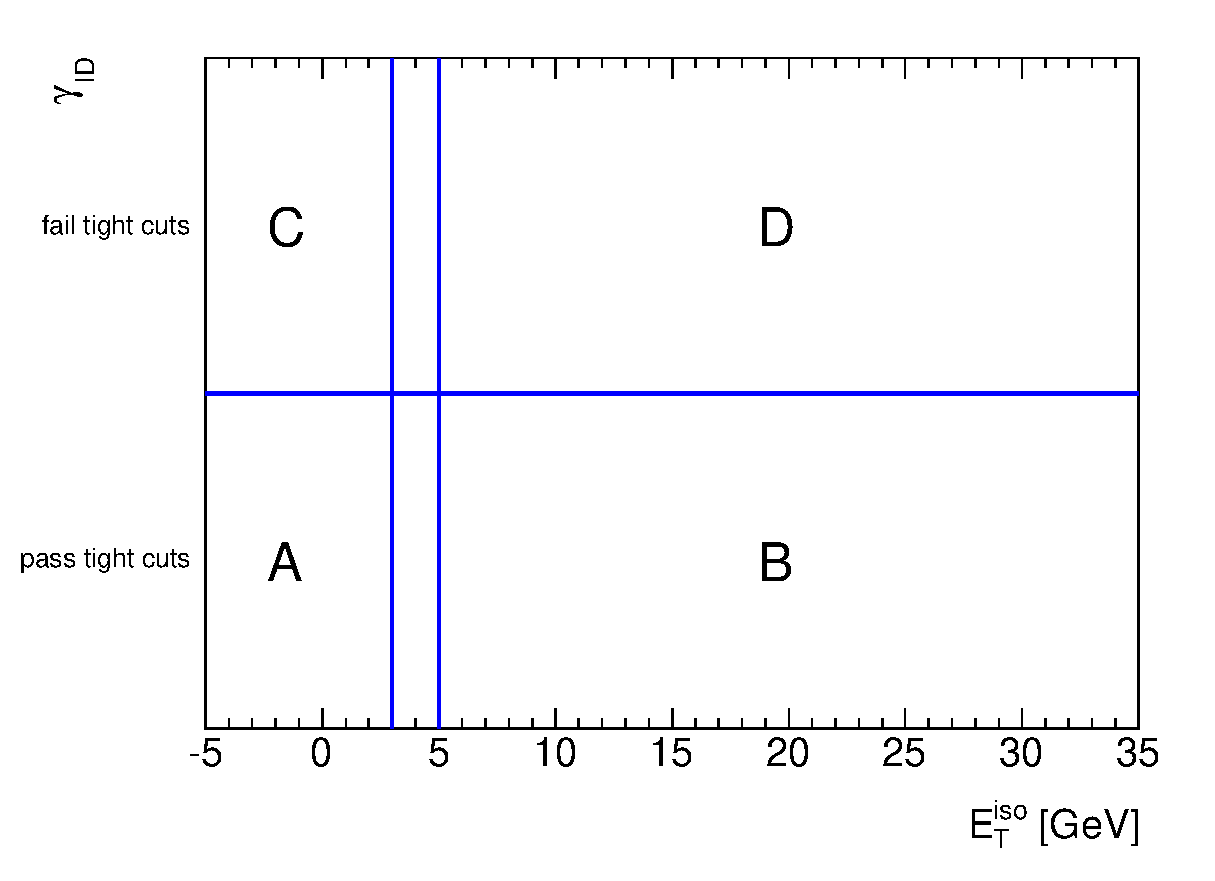
\includegraphics[scale=0.60]{figures/2dsketch.eps}
  \caption{{\small Illustration of the two-dimensional plane, defined	
      by means of the isolation and a subset of the photon
      identification (ID) variables, from the observed yields $N_{B},
      N_{C}$ and $N_{D}$ in the three control regions, the background
    yield in the signal region were the observed total signal yield is
    $N_{A}$. Sketch and caption are taken from \cite{}.}}
\label{fig::2dsketch}
\end{figure}

The 2D-sideband method is based on the following two assumptions: 
\begin{enumerate}
\item The signal contamination in the three background control regions (B, C, and D)
is small. This implies that all reconstructed photons falling in
one of these regions are coming from a background event. In particular, the
fraction of events coming from jet-faking events $N^{Z\text{jet}}$ can be
extracted by subtracting the contribution from electroweak backgrounds 
\New{} (estimated from Monte Carlo) from the total number of
observed events in each of these three regions: $N_A = \Nzg{A} + \Nzj{A} + \New{A}$
for the signal region and $N_K = \Nzj{K} + \New{K}$ ($K \in \{B, C, D\}$) 
for each control region.
%
\item The ratio of isolated to non-isolated background candidates from the jet-fake
in the not-tight bins $\left(\frac{\Nzj{D}}{\Nzj{C}}\right)$
is equal to the same ratio computed in the tight bins
$\left(\frac{\Nzj{B}}{\Nzj{A}}\right)$.
\end{enumerate}
These statements imply that the $Z+\text{jets}$ background in region A can
be calculated as follows:
\begin{equation}
    \Nzj{A} = (N_B - \New{B})\frac{(N_C - \New{C})}{(N_D - \New{D})}.
\end{equation}
Thus, the $Z+\gamma$ yield \Nzg{A} in region A is estimated from the number
of events in the data in the four regions as
\begin{equation}
   \Nzg{A} = (N_A - \New{A}) - (N_B - \New{B})\frac{(N_C - \New{C})}{(N_D - \New{D})}.
\end{equation}
where \New{} is estimated from electroweak background Monte Carlo simulations.

However, one must correct for the fact that the number of signal events in the
background control regions is always positive and non-zero by defining the
\emph{signal leakage fractions} $c_K = N_K^{Z\gamma\text{MC}}/N_A^{Z\gamma\text{MC}}$
that can be extracted from simulated $Z+\gamma$ samples. In addition,
there are correlations between the photon isolation variable and the
photon identification quantities that are corrected by a correlation 
coefficient
\begin{equation} 
    R^{Z\text{jetsMC}} = \frac{\Nzjmc{A} \Nzjmc{D}}{\Nzjmc{B} \Nzjmc{C}}
\end{equation}
obtained from high statistics $Z+\text{jets}$ simulated events, after removing
- using the truth information - the contributions from $Z+\gamma$ processes.
The final result for the signal yield is then
\begin{equation}
   \Nzg{A} = (N_A - \New{A}) - (N_B - \New{B} - c_B\Nzg{A})\frac{(N_C - \New{C} - c_C\Nzg{A})}{(N_D - \New{D} - c_D\Nzg{A})}\,R^{Z\text{jetsMC}}.
\label{eq:2destB}
\end{equation}
This is a second-order polynomial equation in $N_A^{Z\gamma}$ that only has
one physical solution, i.e. a positive solution. Finally, the $Z+\text{jets}$
background is obtained as
\begin{equation}
\Nzj{A} = N_A - \New{A} - \Nzg{A}.
\label{eq:2destA}
\end{equation}

\subsection{Data-Monte Carlo Comparisons}
Following the discussion in the previous section the $Z$+jets background to
$Z\gamma$ processes are estimated using Equation~\ref{eq:2destA} and \ref{eq:2destB}.
In the following we define the purity ($P$) of $Z\gamma$ candidate samples as
\[
    P = \frac{N_A - \Nzj{A} - \New{A}}{N_A}.
\]
A summary of the different measured backgrounds as well as the purity of $Z\gamma$
events in data are calculated and summarized in \refT{tab:zgbgsummary}.
After the full selection the relative contributions from the different backgrounds
to the selected data are 82\%, 17\%, and 1\% for $Z+\gamma$, $Z+\text{jets}$ and
$t\bar t$, respectively.
In addition, a comparison between data and the simulation after scaling each 
MC background contribution to the number of events estimated in data is shown in 
\refF{fig:zgamma_mass_linear} and \ref{fig:Dm_mass_linear}. 
A good agreement between data and simulation is observed.

\begin{table}[!htbp]
\centering
\begin{tabular}{ccccccc}
       \hline
%%      \textbf{background source } & $pp \rightarrow e^{+}e^{-}\gamma$  & $pp \rightarrow \mu^{+}\mu^{-}\gamma$ \\
       \textbf{background source } & $Z(e^{+}e^{-})\gamma$  & $ Z( \mu^{+}\mu^{-})\gamma$ \\
       \hline
 	  &   {\bf 8TeV} &  \\
       \hline
	   
      total observed events & 13898    &  16658 \\
       \hline
        $Z$+$jets$             & $ 2137.58 \pm 116.94 \pm 541.45  $ &  $ 2561.69 \pm 109.23  \pm 474.94 $  \\
       $t\bar t$            &  $ 63.08 \pm 2.65 $&  $ 78.58 \pm 3.08 $ \\
 	$WZ $   	     &  $ 9.55 \pm 0.66 $ &  $ 6.97 \pm 0.52 $    \\
       \hline
   extracted $Z\gamma$ events  & $ 11687.79 \pm 166.07  $ &   $ 14010.76 \pm 169.11 $  \\
       \hline
 	Purity   		&  $ 0.841 \pm 0.014 \pm 0.039 $             &  $ 0.841 \pm  0.012 \pm 0.028$    \\
       \hline	 
       \hline
 	  &   {\bf 7TeV} &  \\
       \hline

      total observed events & 1960    &  2665 \\
       \hline
        $Z$+$jets$             & $ 318.20 \pm 45.84 \pm 34.24  $ &  $ 343.25 \pm 39.88  \pm 21.04 $  \\
       $t\bar t$            &  $ 7.45 \pm 1.17 $&  $ 8.31 \pm 1.23 $ \\
        $WZ $                &  $ 5.63 \pm 0.19 $ &  $ 5.38 \pm 0.18 $    \\
       \hline
   extracted $Z\gamma$ events  & $ 1628.72 \pm 63.74  $ &   $ 2308.06 \pm 65.25 $  \\
       \hline
        Purity                  &  $ 0.831 \pm 0.037 \pm 0.017 $             &  $ 0.866 \pm  0.030 \pm 0.015$    \\
   \hline
   \hline
      

\end{tabular}
\caption{
 Estimations of $Z$+jets and electroweak background events after all $H\rightarrow Z \gamma$ selection cuts in electron and muon categories for the 2012 and 2011 datasets, which have luminosities around 20.7 fb$^{-1}$ and 4.6 fb$^{-1}$, respectively. Errors in MC $t\bar{t}$, $WZ$ and extracted Data-Driven $Z\gamma$ events are only statistical.}
  \label{tab:zgbgsummary}
\end{table}

\begin{figure}[!htbp]
  \begin{center}
    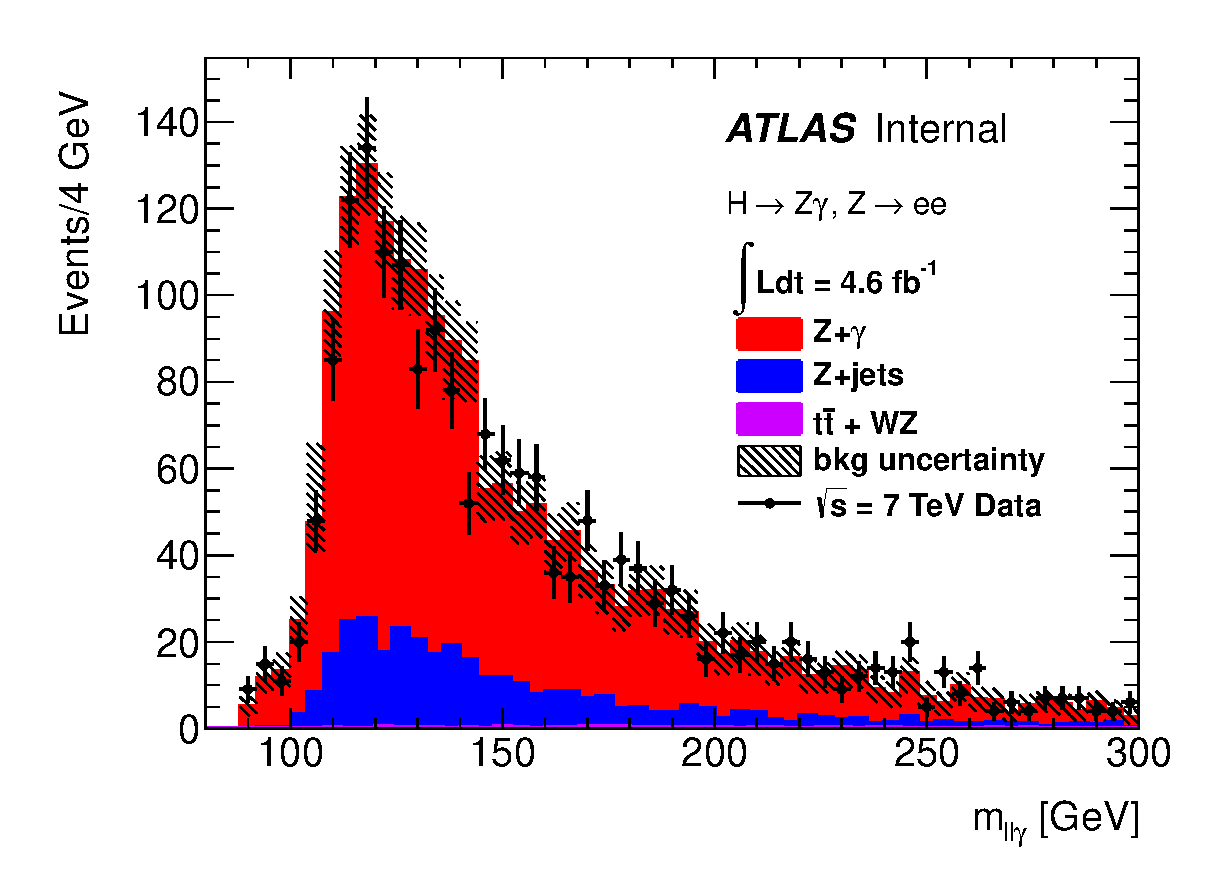
\includegraphics[width=0.49\columnwidth]{figures/bkg_decomposition_2011_e_Mllg_Z_PV_corr_linscale}
    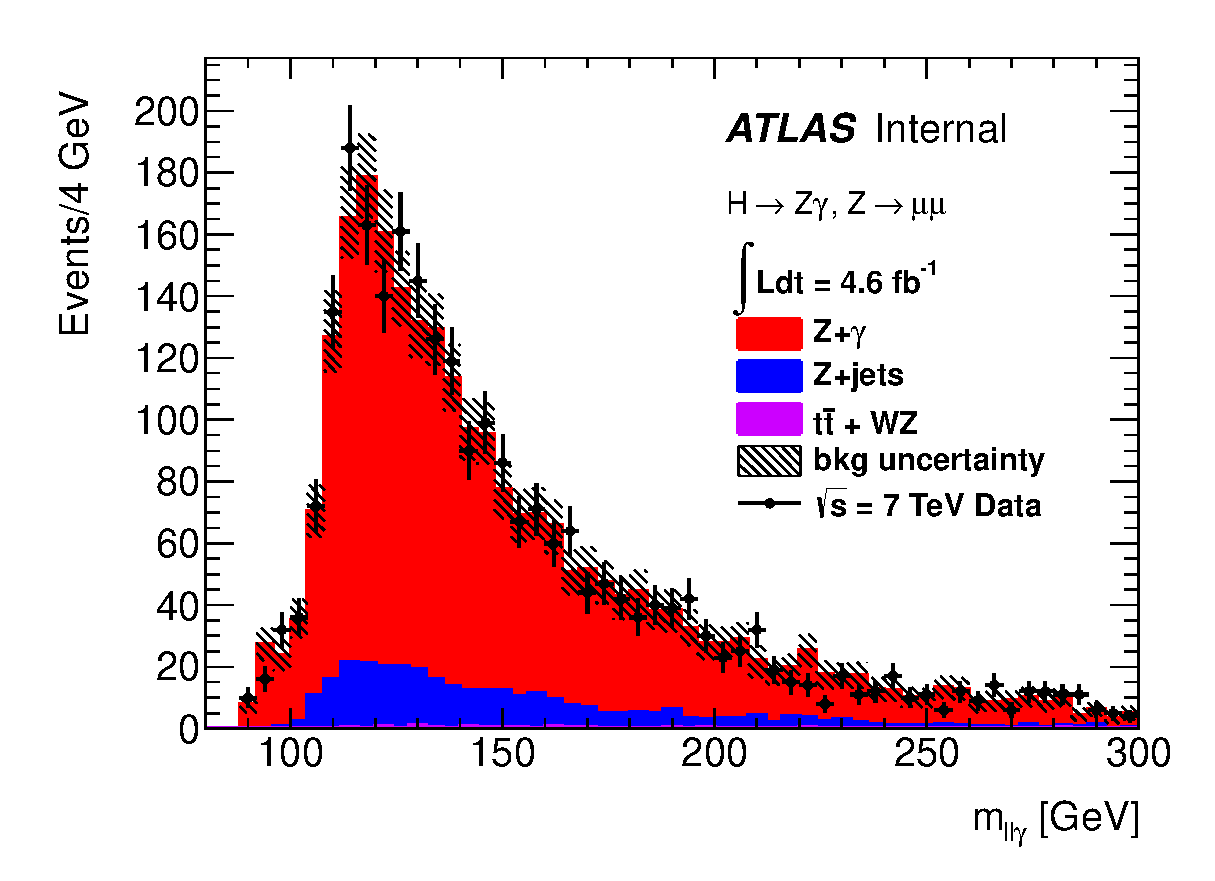
\includegraphics[width=0.49\columnwidth]{figures/bkg_decomposition_2011_mu_Mllg_Z_PV_corr_linscale}
    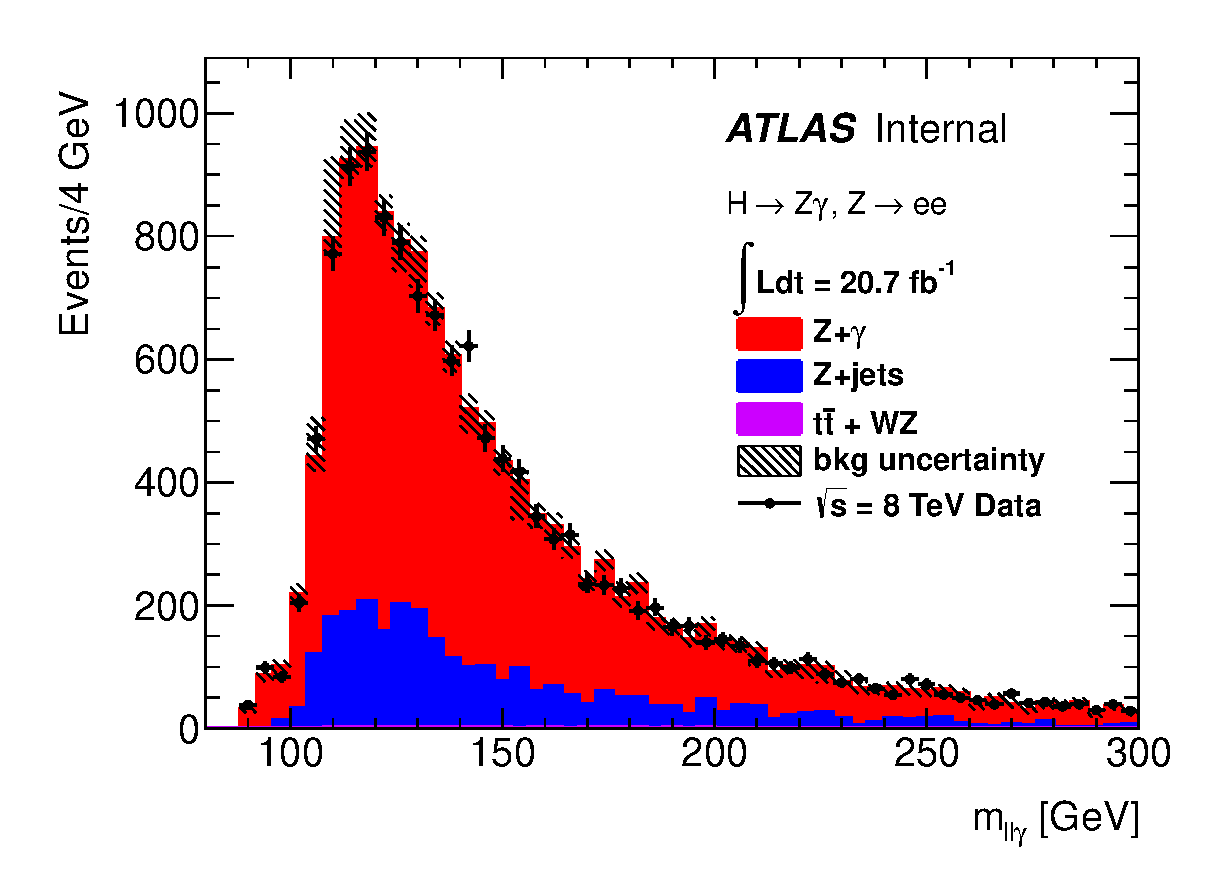
\includegraphics[width=0.49\columnwidth]{figures/bkg_decomposition_2012_e_Mllg_Z_PV_corr_linscale}
    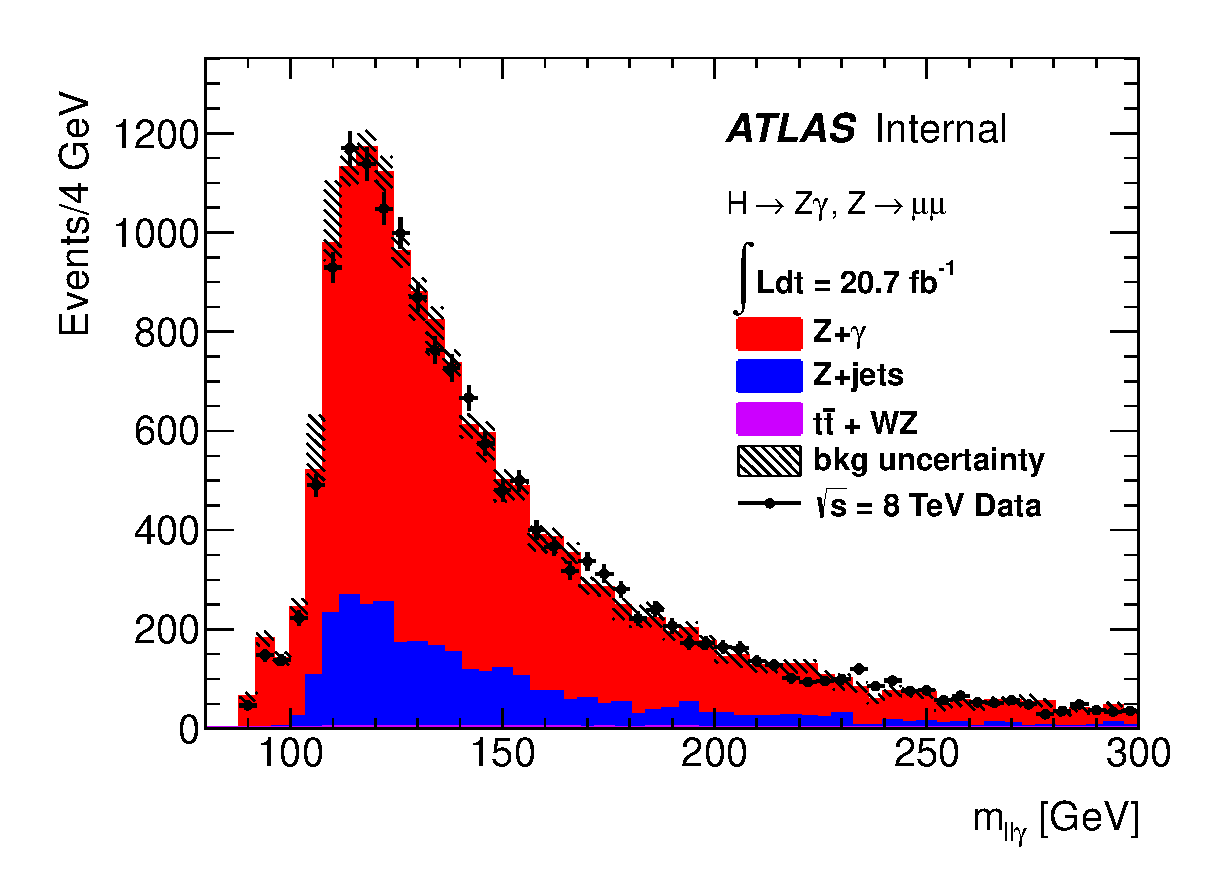
\includegraphics[width=0.49\columnwidth]{figures/bkg_decomposition_2012_mu_Mllg_Z_PV_corr_linscale}
    \caption{Three-body invariant mass $(m_{\ell\ell\gamma})$ distribution 
      of selected events in data (dots) and from the various
      background sources (histograms, from the simulation) normalized 
      to the yields determined as described in the text, 
      for $Z\to ee$ (left) and $Z\to\mu\mu$ (right) channels.
      The small peak near $m_Z$ is from residual FSR $Z$+$\gamma$ contamination.
      The background uncertainty includes statistical uncertainties and 
      systematic uncertainties from the inputs taken from the simulation, as detailed in the text.
    }
    \label{fig:zgamma_mass_linear}
  \end{center}
\end{figure}

\begin{figure}[!htbp]
  \begin{center}
    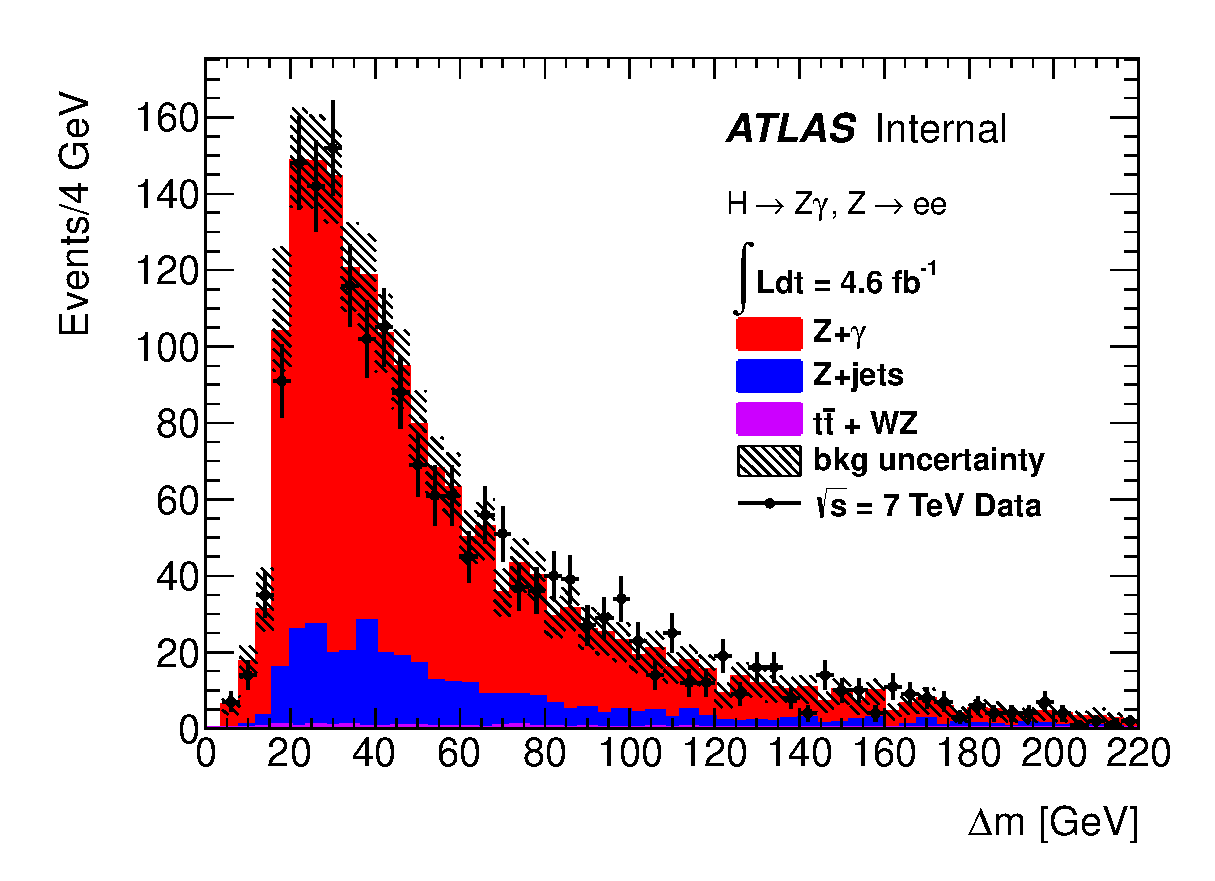
\includegraphics[width=0.49\columnwidth]{figures/bkg_decomposition_2011_e_dMllg_Z_PV_corr_linscale}
    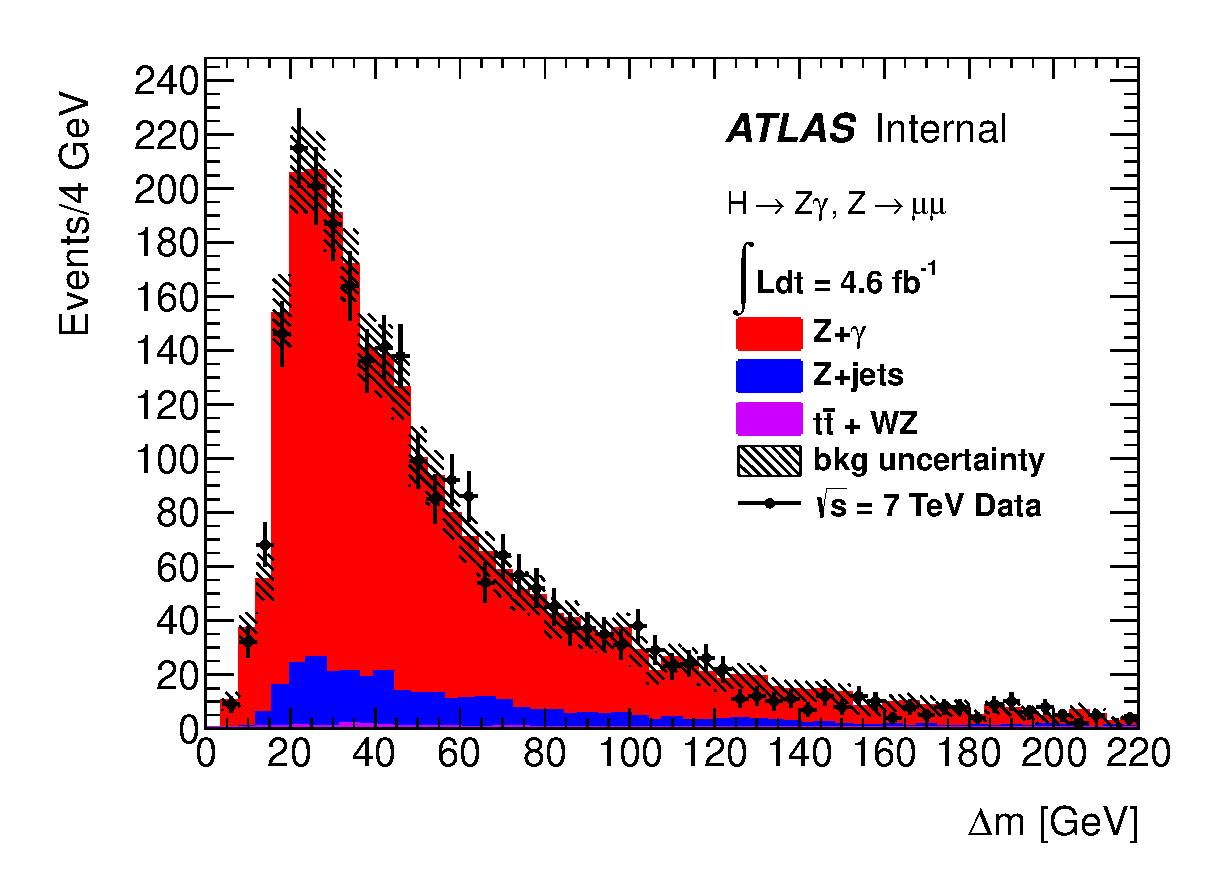
\includegraphics[width=0.49\columnwidth]{figures/bkg_decomposition_2011_mu_dMllg_Z_PV_corr_linscale}
    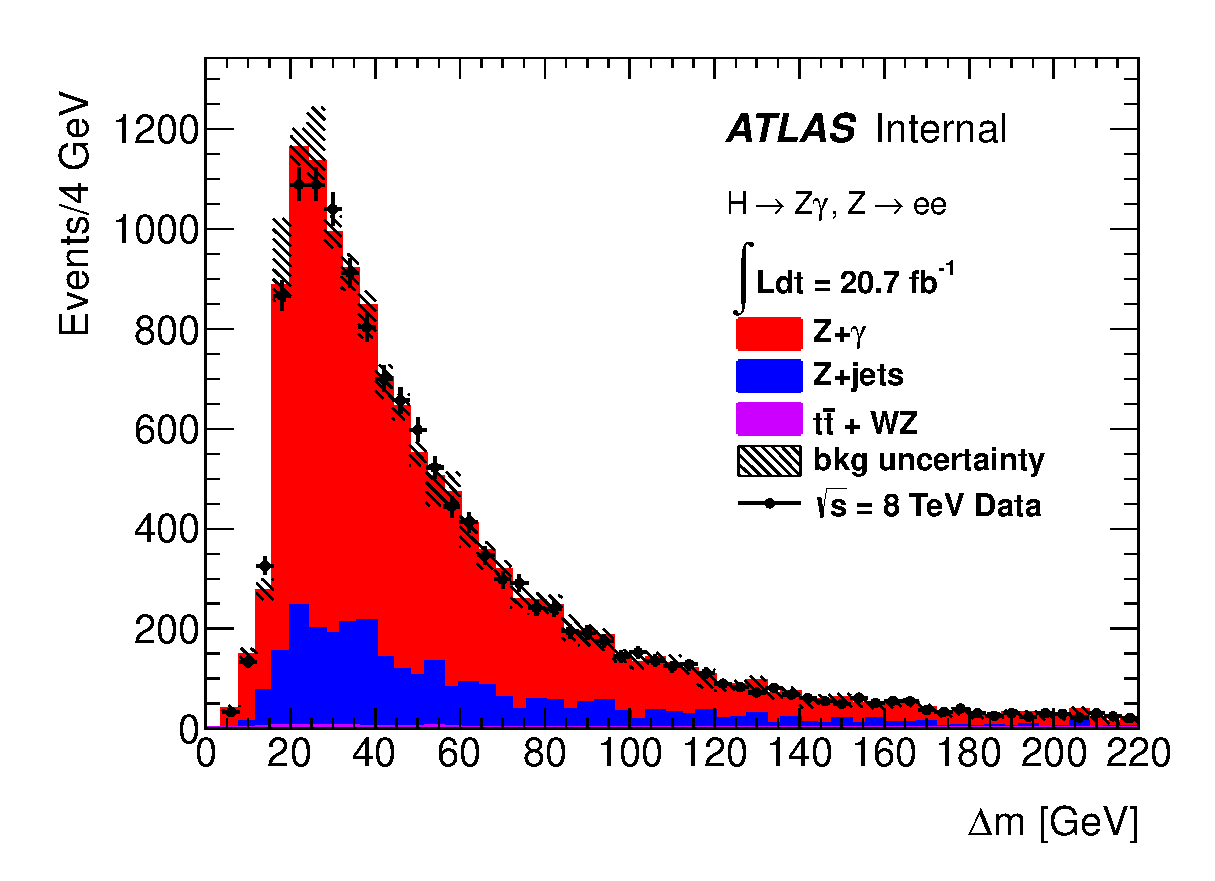
\includegraphics[width=0.49\columnwidth]{figures/bkg_decomposition_2012_e_dMllg_Z_PV_corr_linscale}
    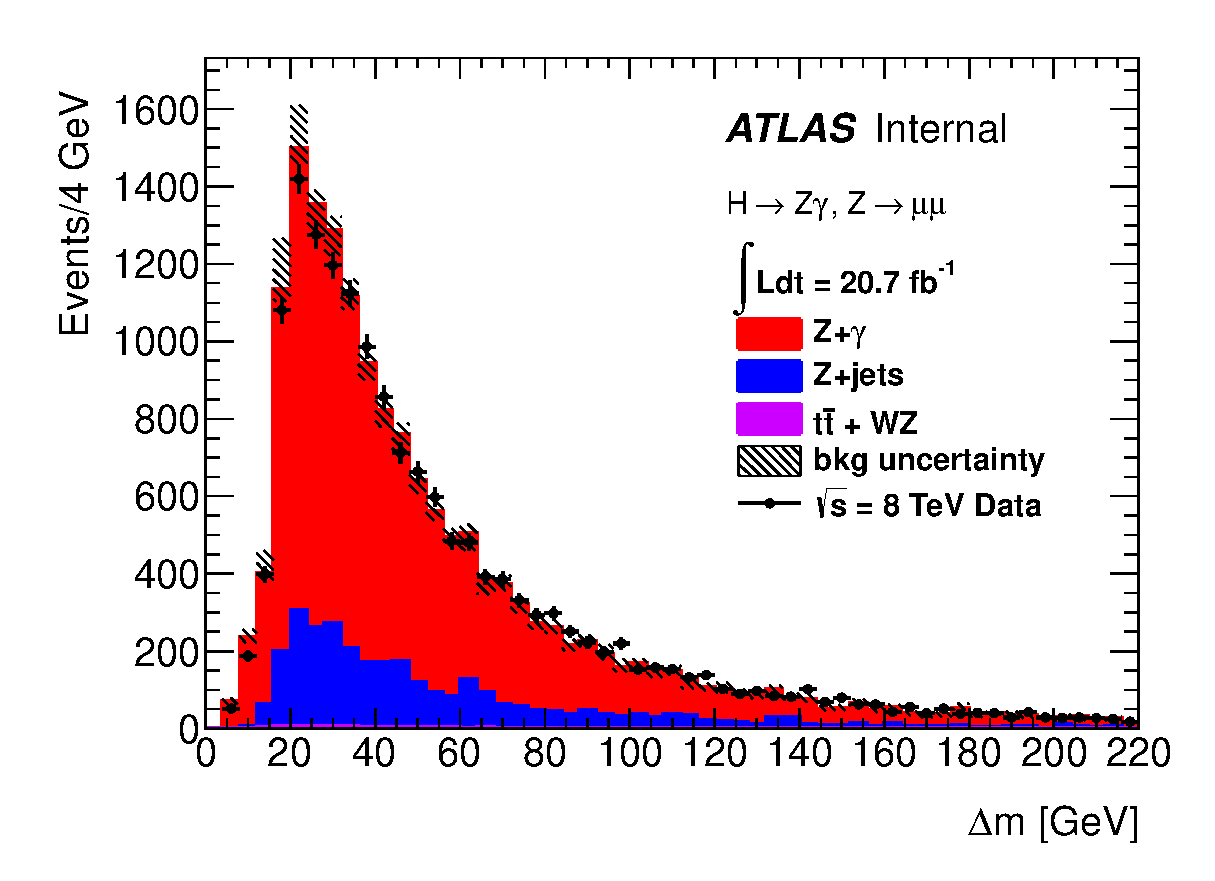
\includegraphics[width=0.49\columnwidth]{figures/bkg_decomposition_2012_mu_dMllg_Z_PV_corr_linscale}
    \caption{Distribution of the difference $\Delta m$ 
      between the final state three-body invariant mass
      $m_{\ell\ell\gamma}$ and the di-lepton invariant mass
      $m_{\ell\ell}$ for selected events in data (dots) and from
      the various background sources (histograms) normalized to the yields determined 
      as described in the text, for $Z\to ee$ (left) and $Z\to\mu\mu$ (right) channels.
      The background uncertainty includes statistical uncertainties and systematic
      uncertainties from the inputs taken from the simulation.
    }
    \label{fig:Dm_mass_linear}
  \end{center}
\end{figure}

\label{sec:compare}

\section{Signal Studies}
\label{sec:signal}
The various properties of the \HToZg signal are described in this section.
This includes a discussion of the number of signal events expected to be
observed in data (expected signal yield) followed by a description
of the template model used to describe the signal's shape in data.

\subsection{Expected signal yield}
An understanding of the expected signal yield follows the same calculation
described in \refS{subsec:prodproc} with an additional term that accounts
for the fact that the selection described in \refS{sec:event} will not
select all of the \HTollg events produced by the LHC. As described in
\refS{subsec:mc}, Higgs boson production and decay are simulated with
several Monte Carlo samples that are passed through a full detector simulation.
This full simulation allows for the estimation of the signal selection efficiency
and therefore the expect signal yield for a SM Higgs boson decaying to $Z\gamma$
in each decay mode ($i = gg$, VBF, etc.) via:
\[
    N_{i,\ell}(m_H) = \int L\, dt \times \sigma_i(m_H) \times 
    B_{H\to Z\gamma}(m_H) \times B_{Z\to\ell\ell} \times \epsilon_{i,\ell}(m_H)
\]
where
\begin{enumerate}
 \item $\int L\, dt$ is the integrated luminosity of the data sample,
 \item $\sigma_i(m_H)$ is the SM Higgs boson production cross section for a
 Higgs boson of mass $m_H$, in the production process $i$ ($gg$, VBF, etc.),
 \item $B_{H\to Z\gamma}$ is the branching fraction for the decay to $Z\gamma$
 of a SM Higgs boson of mass $m_H$,
 \item $B_{Z\to\ell\ell} = (3.3658 \pm 0.0023)\%$ is the $Z\to\ell\ell$ branching
 fraction \cite{PDG2012},
 \item $\epsilon_{i,\ell}(m_H)$ is the selection efficiency for \HTollg events.
\end{enumerate}
The second and third inputs are taken from
\cite{LHCHiggsCrossSectionWorkingGroup:2011ti, LHCHiggsCrossSectionWorkingGroup:2012vm}, 
while the fourth input is estimated from the ATLAS full simulation of signal events.
The expected total yield, for each lepton flavor, is then 
\[
    N_{\ell}(m_H) = \sum_i N_{i,\ell}(m_H).
\]

The signal efficiency was computed using signal Monte Carlo as
\[
    \epsilon_{i,\ell} = \frac{\sum_j w^{\text{reco}}_{j,\ell}}{\sum_k w^{\text{true}}_{k,\ell}}
\]
where
\begin{itemize}
 \item $\sum_j w^{\text{true}}_{j,\ell}$ is the sum over the events $j$ in which the
 generated $Z$ boson decays to a $\ell\ell$ pair (identified by inspecting the
 MC truth record) of the product of the `initial' weights\footnote{These are
 the Monte Carlo weights applied before the object reconstruction, i.e. pile-up
 and a $z$-vertex weight}.
 \item $\sum_k w^{\text{reco}}_{k,\ell}$ is the sum over the events $k$ in which
 the generated $Z$ boson decays to a $\ell\ell$ pair and passing the full \HTollg
 selection of the `final' weights\footnote{These are the initial weights and the 
 efficiency scale factors for the trigger, the leptons, and the photon.}.
\end{itemize}
The expected signal yields and selection efficiencies for Higgs boson masses 
between 120 and 150 GeV and for an integrated luminoisty of 20.7 \ifb (4.6 \ifb)
at $\rts = 8$ (7) TeV are shown in \refT{tab:expected_signalyields}.

\begin{table}[!htbp]
  \begin{center}
  \caption{Selection efficiency ($\varepsilon$) and number of expected
    $H\to Z\gamma$ signal events ($S$),
    for Higgs boson masses between 120 and 150 GeV,
    for the two reconstructed $Z$ boson final states and
    for \lumiseventev~\ifb\ at $\sqrt{s}=7\TeV$
    and \lumieighttev~\ifb\ at $\sqrt{s}=8\TeV$.
    The relative statistical uncertainty on the quoted numbers
    is around 1\%.
    %% The relative uncertainty on the selection efficiency is
    %% around 5\%, as described in Section~\ref{sec:Systematics}.
    %% The relative uncertainty on the signal yield
    %% also includes an additional 3.6\% (1.8)\% contribution
    %% from the luminosity uncertainty in 8 (7) TeV data.
  }
  \label{tab:expected_signalyields}
    \begin{tabular}{l|cc|cc|cc|cc}
\hline
\hline
$m_H$  & \multicolumn{2}{c|}{$Z\to ee$, 7 TeV} & \multicolumn{2}{c|}{$Z\to \mu\mu$, 7 TeV} & \multicolumn{2}{c|}{$Z\to ee$, 8 TeV} &  \multicolumn{2}{c}{$Z\to \mu\mu$, 8 TeV} \\
$[$GeV$]$ & $\varepsilon$ [\%] & $S$ & $\varepsilon$ [\%] & $S$ & $\varepsilon$ [\%] & $S$ & $\varepsilon$ [\%] & $S$ \\
\hline
120  &  17.1  &  0.6  &  22.5  &  0.7  &  21.3  &  4.0  &  25.8  &   4.9  \\
125  &  20.4  &  0.9  &  26.5  &  1.1  &  24.6  &  5.9  &  29.7  &   7.2  \\
130  &  23.0  &  1.1  &  29.9  &  1.5  &  27.3  &  7.7  &  32.8  &   9.3  \\
135  &  25.1  &  1.3  &  32.4  &  1.7  &  29.4  &  9.0  &  35.1  &  10.7  \\
140  &  26.6  &  1.4  &  34.1  &  1.8  &  30.9  &  9.5  &  36.6  &  11.3  \\
145  &  27.5  &  1.4  &  35.0  &  1.8  &  31.7  &  9.2  &  37.3  &  10.8  \\
150  &  27.9  &  1.2  &  35.1  &  1.5  &  32.0  &  8.1  &  37.2  &   9.4  \\
        \hline\hline
    \end{tabular}
  \end{center}
\end{table}

\subsection{Signal model}
The search for the SM Higgs boson decaying to $Z\gamma$ is performed through
a fit to the distribution of an observable that discriminates between signal
and background. Two observables have been studied: the three-body invariant
mass of the final state particles, $m_{\ell\ell\gamma}$,
and the difference between the three-body
and the di-lepton invariant masses, $\dm = \mllg - \mass{\ell}$.
A choice of \dm over \mllg as the discriminating observable was made for the 
following two reasons: \dm is unaffected by the lepton energy scale uncertainties, and
it is to a large extent insensitive to the contribution from FSR in $H\to\mu\mu$
decays.

In the fit, a model for the signal and background probability density functions of
the observable under study is needed. It has been found that both observables
\mllg and \dm of signal events generated at a fix Higgs boson nominal mass are
well described by a composite model of a Crystal Ball function (CB) (a gaussian
core\footnote{A gaussian is used instead of a Lorentzian peak because of the
restricted resolution of the ATLAS detector.} 
with one exponential tail modeling energy loss due to final-state photon
radiation) \cite{Oreglia}, 
and a small wide Gaussian component (GA) modeling the distribution's outliers.
The formula for the CB function is given as follows:
\begin{displaymath}
    CB(m_H) = \left\{
            \begin{array}{lr}
            \frac{N}{\sqrt{2 \pi \sigma}} \exp\left(-\frac{(\mllg-m_H)^2}{2\sigma^2}\right), & \qquad \mathrm{for}\quad \frac{\mllg-m_H}{\sigma} > -\alpha; \\
            \frac{N}{\sqrt{2\pi\sigma}} \left(\frac{n}{|\alpha|}\right)^n \exp\left(-\frac{|\alpha|^2}{2}\right)\left(\frac{n}{|\alpha|} - |\alpha| - \frac{\mllg - m_H}{\sigma}\right)^{-n}, & \qquad \mathrm{for}\quad \frac{\mllg-m_H}{\sigma} \le -\alpha.
            \end{array}
               \right.
\end{displaymath}
where $N$ is a normalization parameter, and $m_H$ is the Higgs boson mass.

Since the parameters describing the signal model can also be a function
of the Higgs boson mass, a complete description of the signal in the whole
mass range is a function that incorporates these variations. The global
resolution model is such an analytic function of the mass given as
\[
    R(m_{\ell\ell\gamma}, \mu_{CB}, \sigma_{CB}, n_{CB}, \mu_{GA}, \sigma_{GA}) =
    f_{CB} \cdot CB\left[m_{\ell\ell\gamma}, \mu_{CB}, \alpha_{CB}, f_{CB},
    \sigma_{CB}, n_{CB}\right] + (1 - f_{CB}) \cdot
    GA\left[m_{\ell\ell\gamma}, \mu_{GA}, \sigma_{GA}\right]
\]
where $\sigma_{CB}, \mu_{CB}$ and $\sigma_{GA}, \mu_{GA}$ represent the
three-body invariant mass resolution and mean value of the core and outliers
respectively. Also $n_{CB}$ and $\alpha_{CB}$ parameterize the non-Gaussian tail, and
$f_{CB}$ is the fraction of the Crystal Ball function in the composite model.

From the available signal Monte Carlo samples at different mass points the parameters
that depend on the nominal Higgs boson mass $m_H$ were identified and the global
and mass dependent parameters were extracted from a simultaneous fit. For the mass
dependent parameters ($\mu_{CB}, \alpha_{CB}, \sigma_{CB}$) we assume a linear
dependence and fit the parameters
\[
\mu_{CB} = \mu_{CB}(m_H = 125 \GeV) + \Delta \mu_{CB}^{\text{slope}} \times \left(\mllg - 125 \GeV \right)
\]
\[
\sigma_{CB} = \sigma_{CB}(m_H = 125 \GeV) + \Delta \sigma_{CB}^{\text{slope}} \times \left(\mllg - 125 \GeV \right)
\]
\[
\alpha_{CB} = \alpha_{CB}(m_H = 125 \GeV) + \Delta \alpha_{CB}^{\text{slope}} \times \left(\mllg - 125 \GeV \right)
\]
The other parameters ($f_{CB}$, $n_{CB}$) are set at a single global value for all
mass points. Also, the relative width of the core and outlier components are shown
to remain unchanged at all mass points, so can be set at a global value.

In total, 7 parameters per category (3 shape parameters with linear dependence of
the Higgs boson mass and 4 global parameters), are extracted from a single fit to
all available Monte Carlo samples, and are sufficient to provide a robust 
parameterization of the invariant mass probability distribution function (p.d.f.)
at any Higgs mass.

\subsection{Fits to signal Monte Carlo samples}

\refF{fig:signal_resolution_corrections} shows the expected mass distribution for
a Higgs boson with a mass of 125 GeV at $\rts = 8 \GeV$ 
after applying all analysis cuts and corrections.
In addition, an example of the distribution of the mass difference 
\dm for signal events passing the full selection for $m_H = 125  \GeV$ is shown in 
\refF{fig:resolution_model_example_8tev_H125}.

\begin{figure}[!htbp]
  \begin{center}
%  {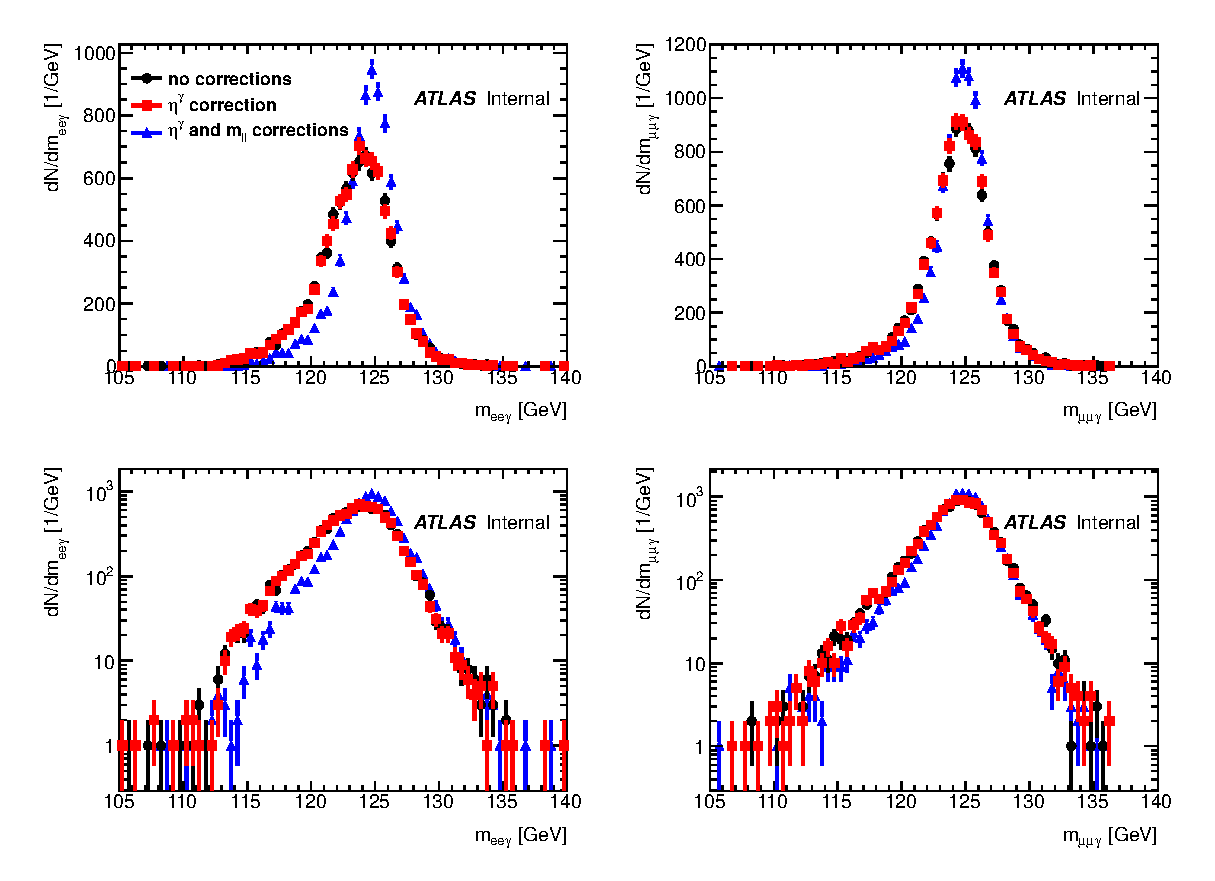
\includegraphics[width=0.99\textwidth]{figures/signal_mllg_corrections}}
{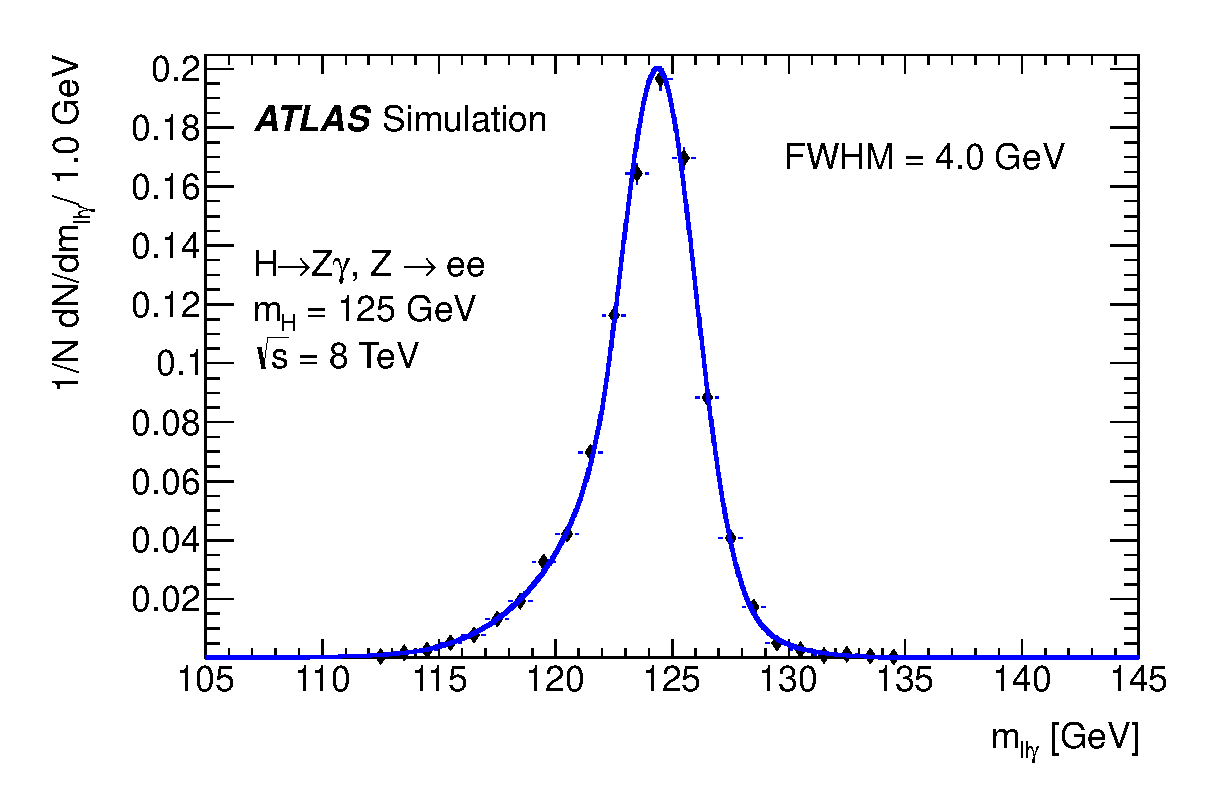
\includegraphics[width=0.48\textwidth]{figures/PlotsSuperposedResolutionCorrections_e_mc12a_Mllg}}
{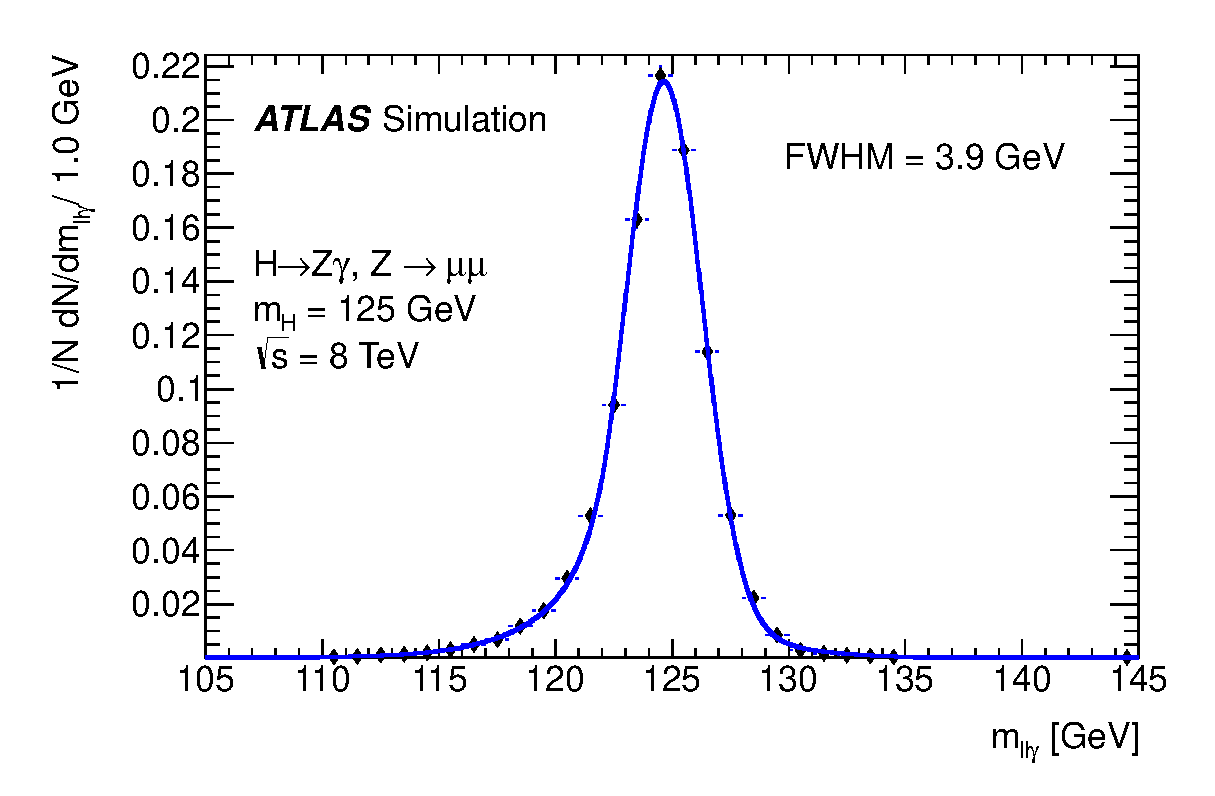
\includegraphics[width=0.48\textwidth]{figures/PlotsSuperposedResolutionCorrections_mu_mc12a_Mllg}}
\caption{Three-body invariant mass distribution for $gg\to H\to Z\gamma$
    selected events in the 8 TeV, $m_H=125$~GeV signal simulation, 
    after applying all analysis cuts and corrections. The blue solid lines 
    represent the fits to the points of the sum of a 
    Crystal Ball lineshape and a Gaussian function.
    Left: $Z\to ee$ channel, Right: $Z\to\mu\mu$ channel.}
%the standard reconstruction (red circles), and after choosing the event primary vertex as the photon origin and applying the $Z$ mass constraint to the lepton four momenta (blue diamonds). The (dashed) red line and the (blue) solid line  represent the fits to the points of the sum of a Crystal Ball lineshape and a Gaussian function. Left: $Z\to ee$ channel, right: $Z\to\mu\mu$ channel.}
  \label{fig:signal_resolution_corrections}
  \end{center}
\end{figure}

\begin{figure}[!htbp]
  \begin{center}
  {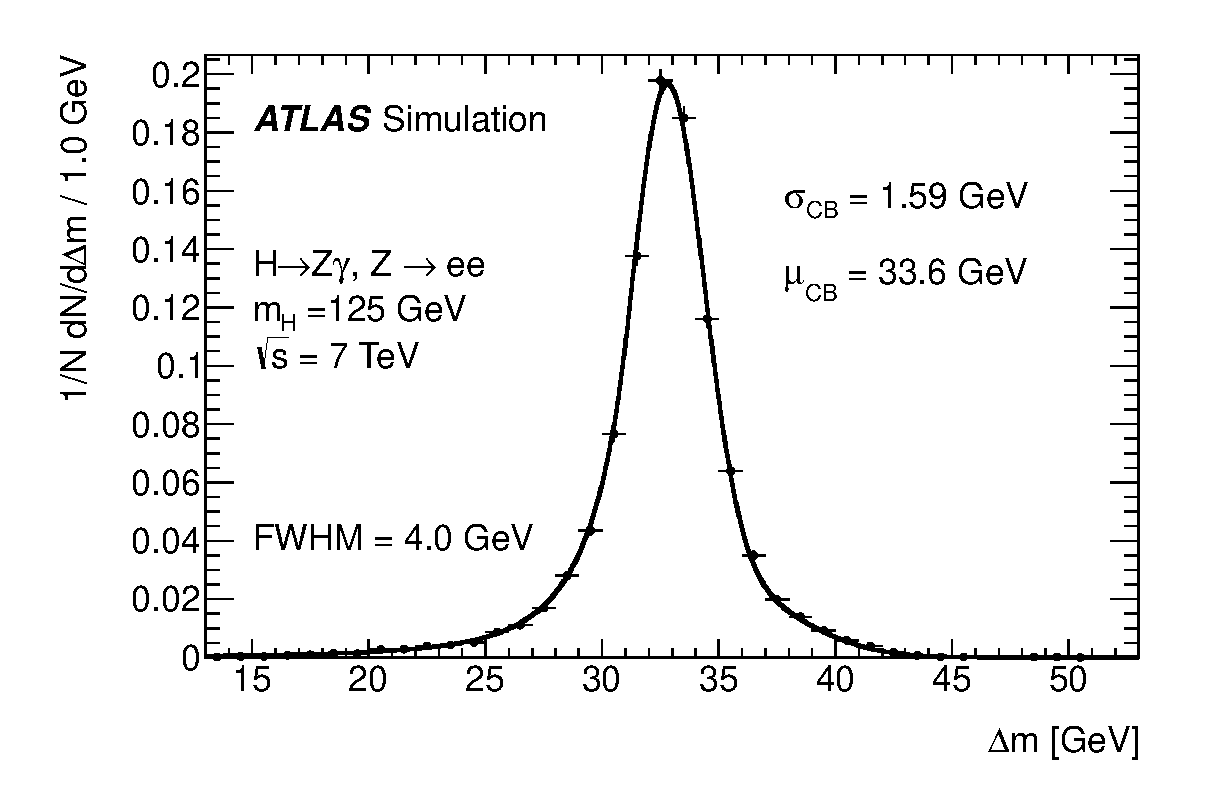
\includegraphics[width=0.46\textwidth]{figures/linPlot_125_EtaZgamma_Cat0_all_e_mc11c_mDif}}
  {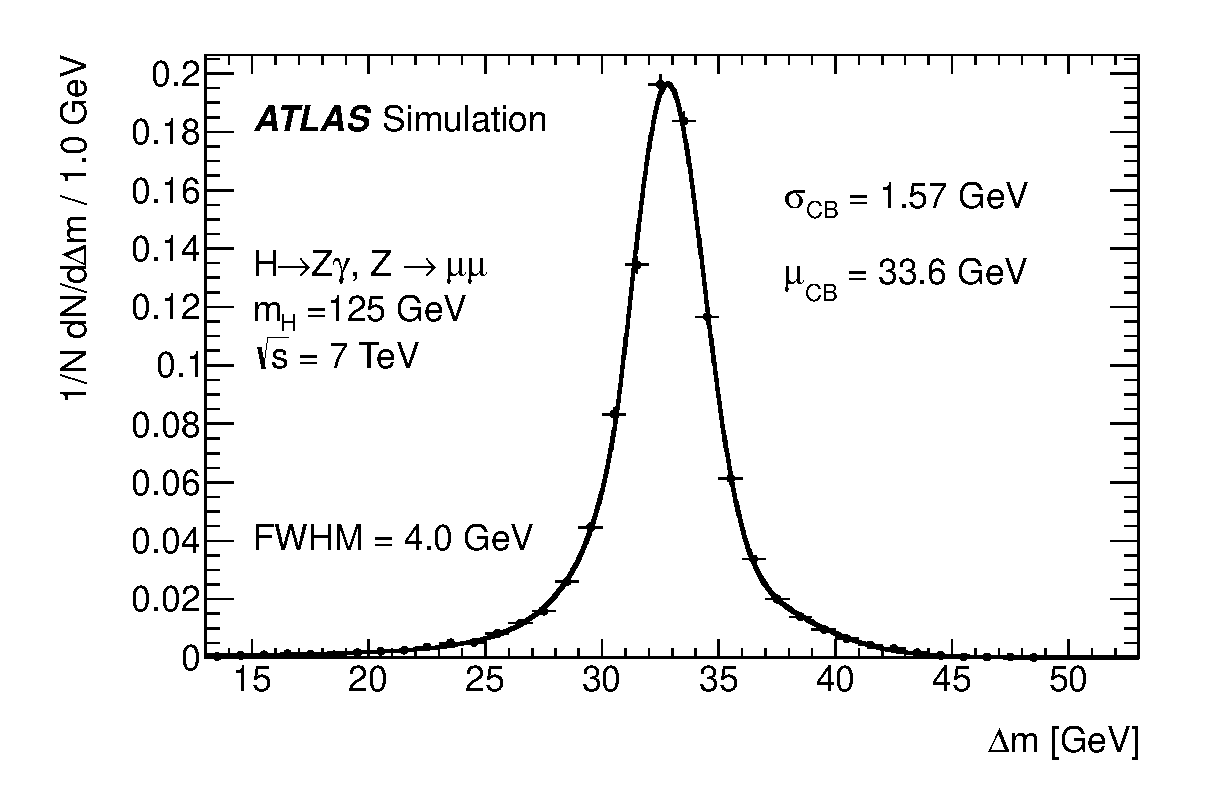
\includegraphics[width=0.46\textwidth]{figures/linPlot_125_EtaZgamma_Cat0_all_mu_mc11c_mDif}}
  {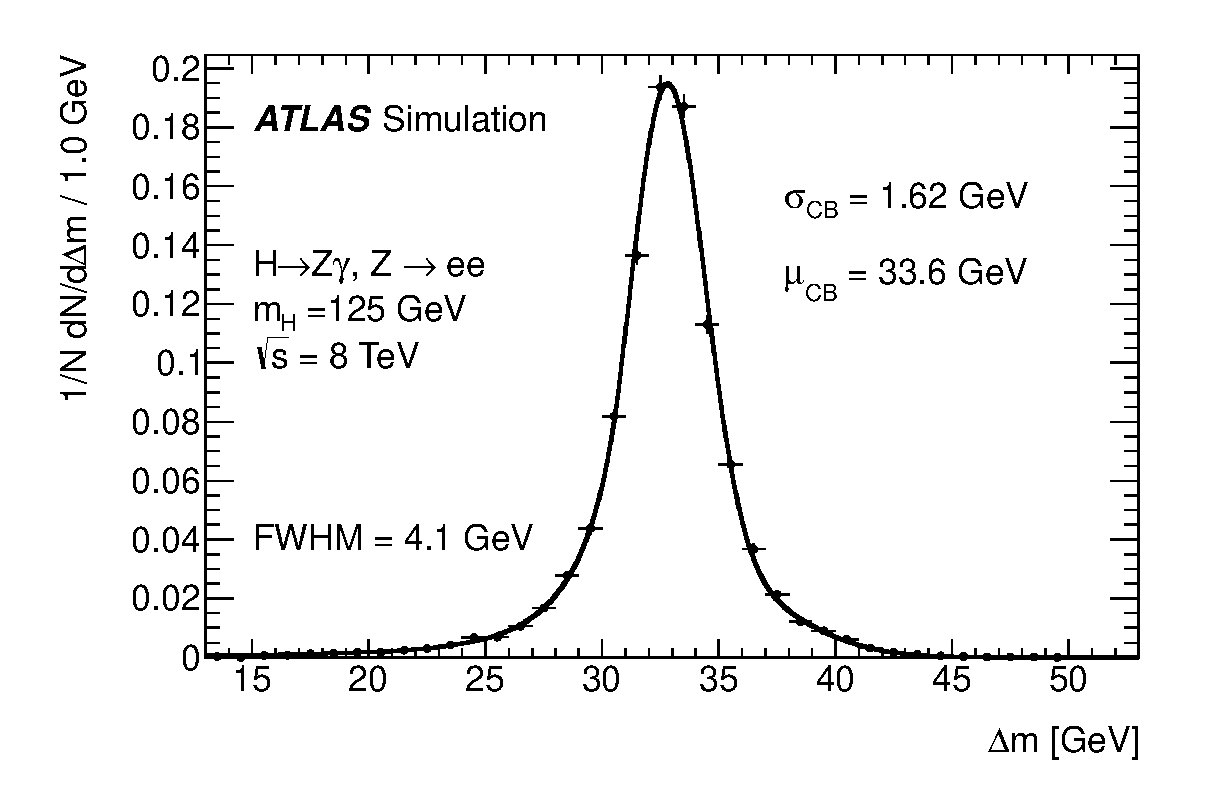
\includegraphics[width=0.46\textwidth]{figures/linPlot_125_EtaZgamma_Cat0_all_e_mc12a_mDif}}
  {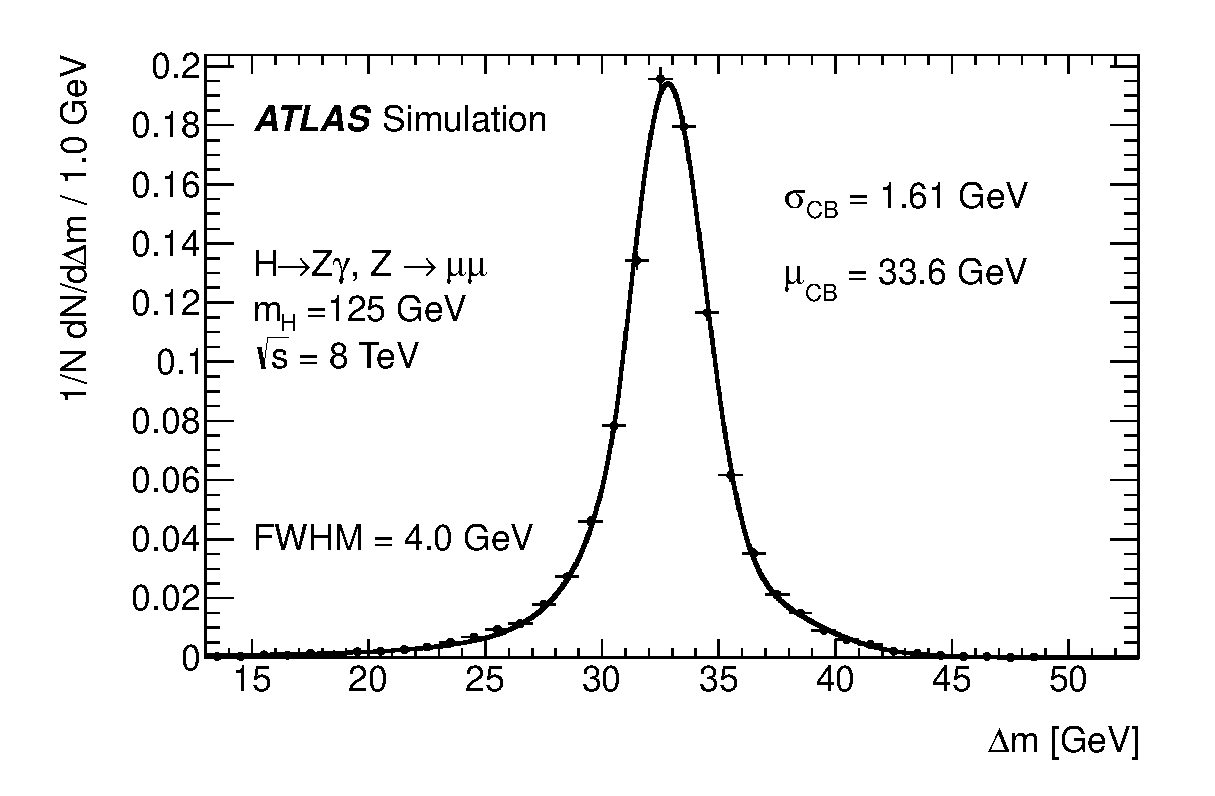
\includegraphics[width=0.46\textwidth]{figures/linPlot_125_EtaZgamma_Cat0_all_mu_mc12a_mDif}}
    \caption{Distribution (normalized to unit area) of the difference $\Delta m$ 
      between the final state three-body invariant mass
      $m_{\ell\ell\gamma}$ and the di-lepton invariant mass
      $m_{\ell\ell}$ for signal events
      passing the full selection (dots), for $m_H = 125$~GeV and $\sqrt{s}=7$ (top) or 8 (bottom) TeV. 
      The line overlaid represents the fit of the distribution with a
      model composed of the sum of a Crystal Ball (CB) and a Gaussian (GA) function.
      Left: electron channel, right: muon channel. 
    }
    \label{fig:resolution_model_example_8tev_H125}
  \end{center}
\end{figure}


\label{sec:signal}

\section{Background Studies}
 \label{sec:background}
In order to distinguish the Higgs boson signal from the background using \dm
as a discriminant, a model for the background distribution is needed. The background
is modeled with a smooth analytic p.d.f. that reproduces the data as well as the 
mixture of background Monte Carlo samples normalized to the data-driven background 
yields. It should be noted that the parameters of the background p.d.f. are not fixed
from simulation, but are fitted on the data. The model was chosen carefully so that
it does not introduce significant biases on the fitted signal while at the same
time preserving the sensitivity to the search.

\subsection{Background model}
A number of functional forms were tested including polynomials of various orders,
as well as non-polynomial functions such as exponential, Crystal Ball+Gaussian,
and Crystal Ball+Landau distributions. The advantage of non-polynomial functions
is that they do not follow the local peaks and troughs of the mass distribution 
that are a result of statistical fluctuations. A high statistics simulated
background-only Monte Carlo sample was used to test the performance of the
signal+background fits of the \dm distribution. This was done by performing
pseudo-experiments\footnote{Data generated by sampling from a known distribution
using a Monte Carlo sampling method. 
The resulting distribution looks like data from the experiment.} 
with a variable amount of Higgs signal events injected in
the mass range 115-135 GeV. For each experiment an unbinned maximum likelihood
fit is performed for a fixed \mllg, and the number of signal events together
with the fitted parameters are obtained. The key result of these tests is
the \emph{spurious signal}, i.e. the bias on the signal. The spurious signal
is defined as the average fitted number of signal events after subtracting
the input signal events ($\average{S} - S_{\text{generated}}$) in units of the
uncertainty in the fitted number of signal events, $\sigma_S$. In order for the
spurious signal to not give a systematic uncertainty on the final result
that is significant compared to the statistical uncertainty of the measurement
itself, we searched for models that yield, for the tested Higgs mass hypotheses,
a spurious signal which is within $\pm20\%$ of the fitted error on the signal yield.

The results for the background-only simulated samples corresponding to 4.6 \ifb
of 2011 data and 20.7 \ifb of 2012 data in the muon and electron channels are
shown in \refF{fig:spurioussignal}. The model that was found to provide the best 
sensitivity to the signal while limiting
the spurious signal to be within $\pm20\%$ of the fitted signal uncertainty, for
both 4.6 \ifb of 2011 data and 20.7 \ifb of 2012, is a third-order 
Chebychev polynomial in the fit range $24 < \dm < 64 \GeV$.

\begin{figure}[htbp]
    \centering
    \begin{subfigure}[b]{0.45\textwidth}
      \centering
      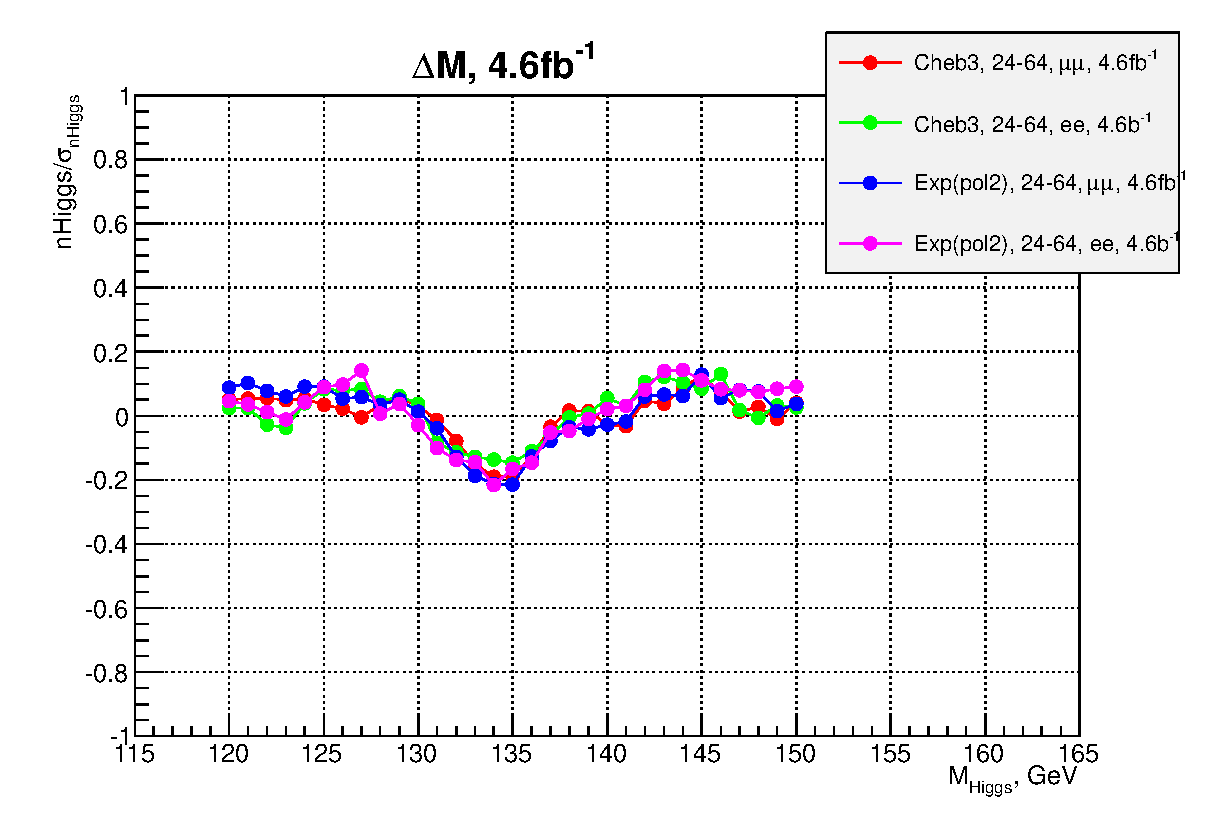
\includegraphics[width=\textwidth]{figures/rat4orig.eps}
      \caption{}
      \label{fig:4spurious}
    \end{subfigure}
    \quad
    \begin{subfigure}[b]{0.45\textwidth}
      \centering
      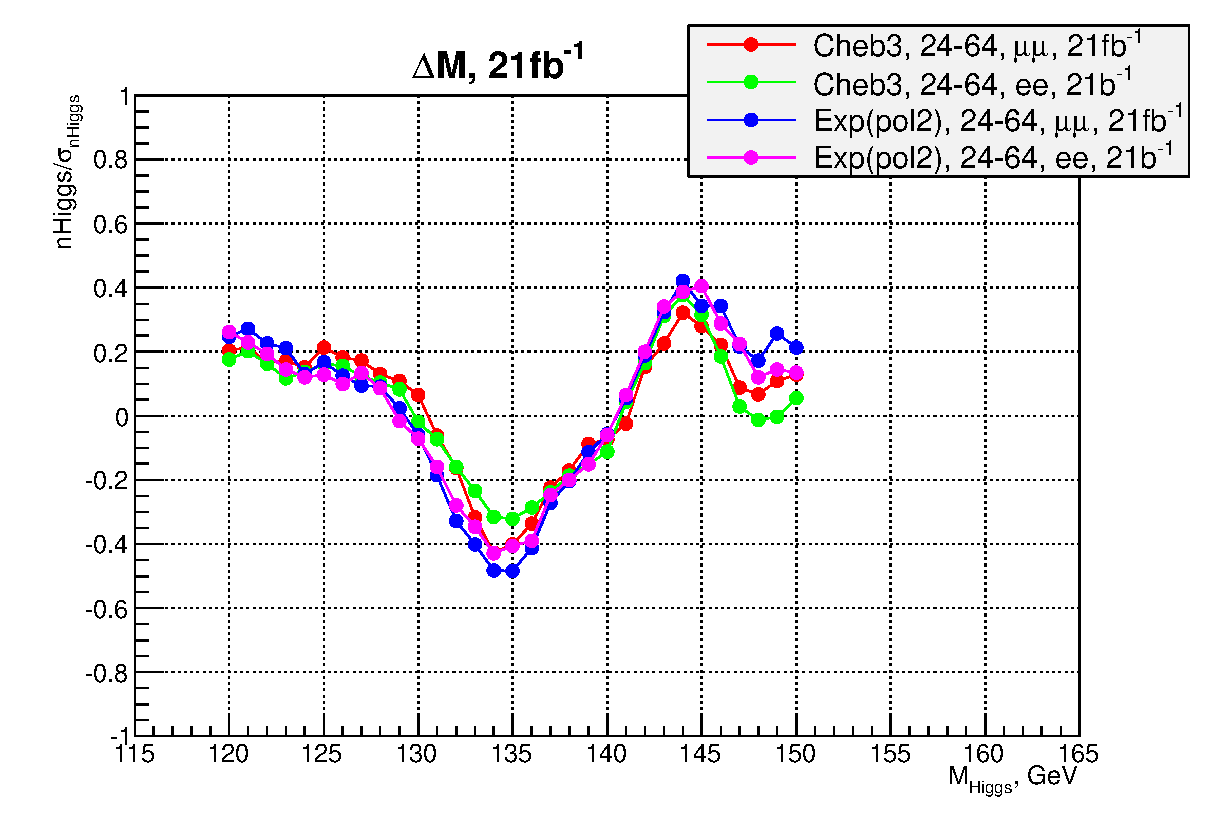
\includegraphics[width=\textwidth]{figures/rat21orig.eps}
      \caption{}
      \label{fig:21spurious}
    \end{subfigure}
    \caption{Number of Higgs candidates divided by uncertainty 
    returned by the fit of the pseudo-data $\Delta M$ distributions averaged over 
    1000 pseudo-experiments with 0 injected Higgs candidates. 
    The statistics corresponds to 4.6 \ifb (Fig.~\ref{fig:4spurious})
    and 21 \ifb (Fig.~\ref{fig:21spurious}). The dip at 135 GeV in the
    $21 \ifb$ sample is due to downward fluctuation in the data at this mass.}
    \label{fig:spurioussignal}
\end{figure}

\subsection{Background-only fits to the data}
The shape parameters and the normalization of the background are determined
by unbinned maximum likelihood fits to the data events selected in the
range $24 \GeV < \dm < 64 \GeV$, performed separately for the two lepton flavors 
and separately for the $\rts = 7 \TeV$ and $\rts = 8 \TeV$ data, using the third-order
Chebychev polynomial selected in the previous section. 
\refF{fig:deltaM_data_bkgonly_fit} shows the background-only fits to the data in the
two categories for the $\rts = 7 \TeV$ and the $\rts = 8 \TeV$ data.

 \begin{figure}[!htbp]
  \begin{center}
    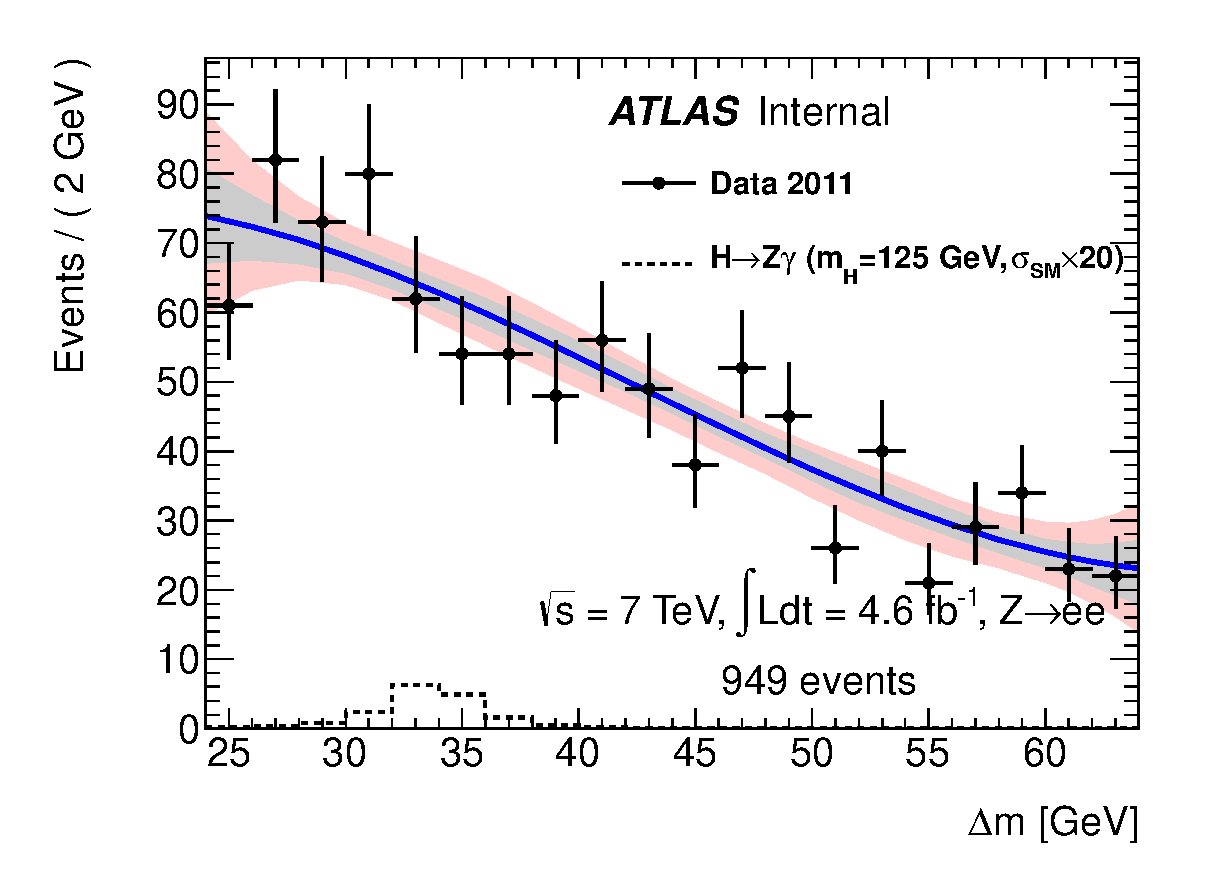
\includegraphics[width=0.49\columnwidth]{figures/bkgplots_e_deltaM_fit_11_CB3_fiterr_internal_withsignal}
    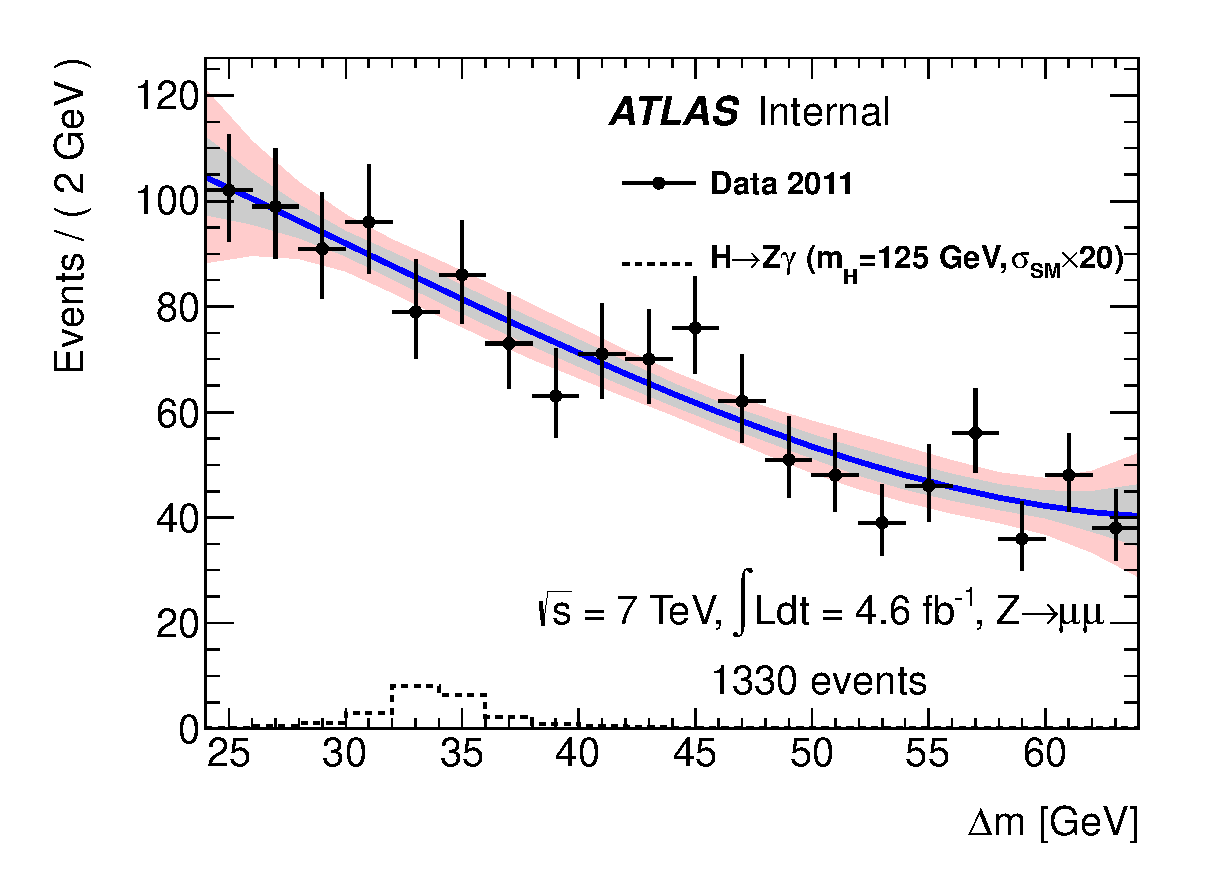
\includegraphics[width=0.49\columnwidth]{figures/bkgplots_mu_deltaM_fit_11_CB3_fiterr_internal_withsignal}
    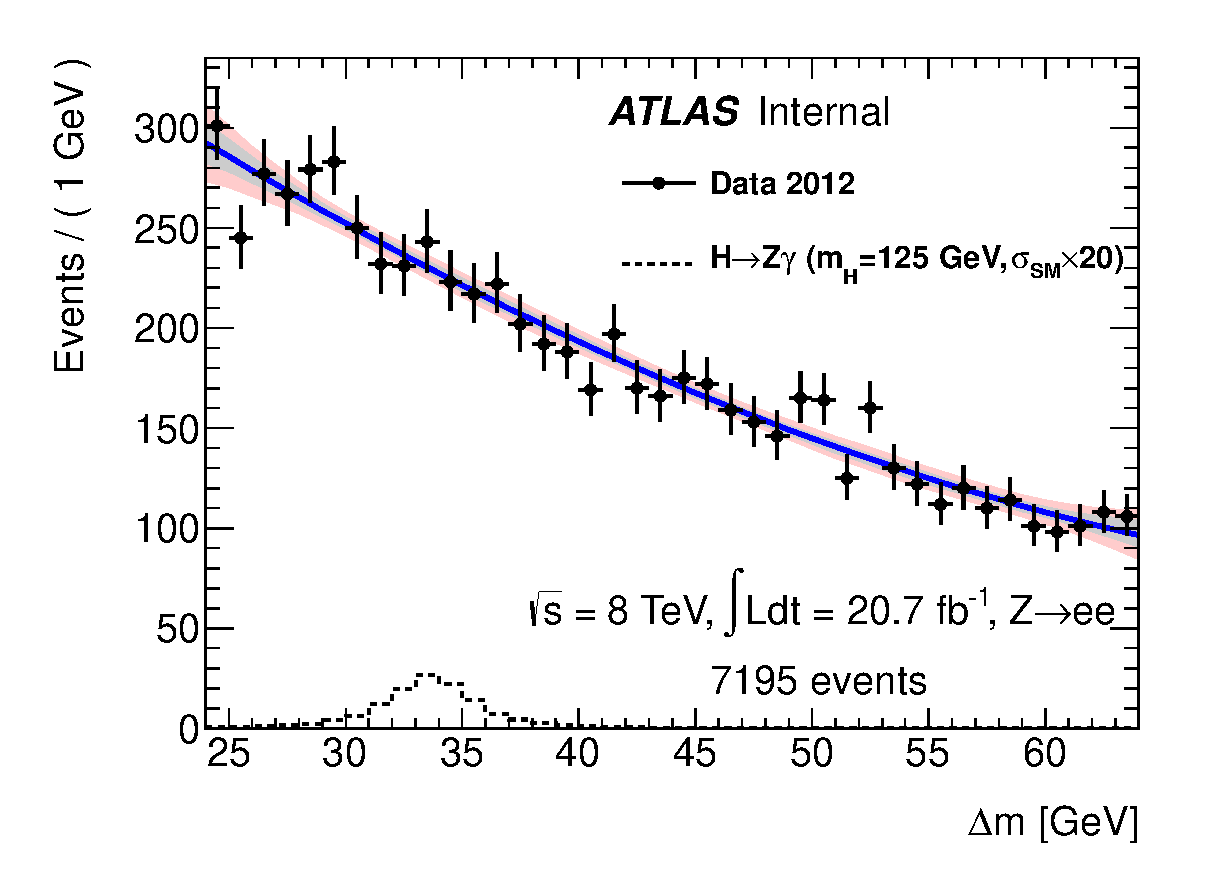
\includegraphics[width=0.49\columnwidth]{figures/bkgplots_e_deltaM_fit_12_CB3_fiterr_internal_withsignal} 
    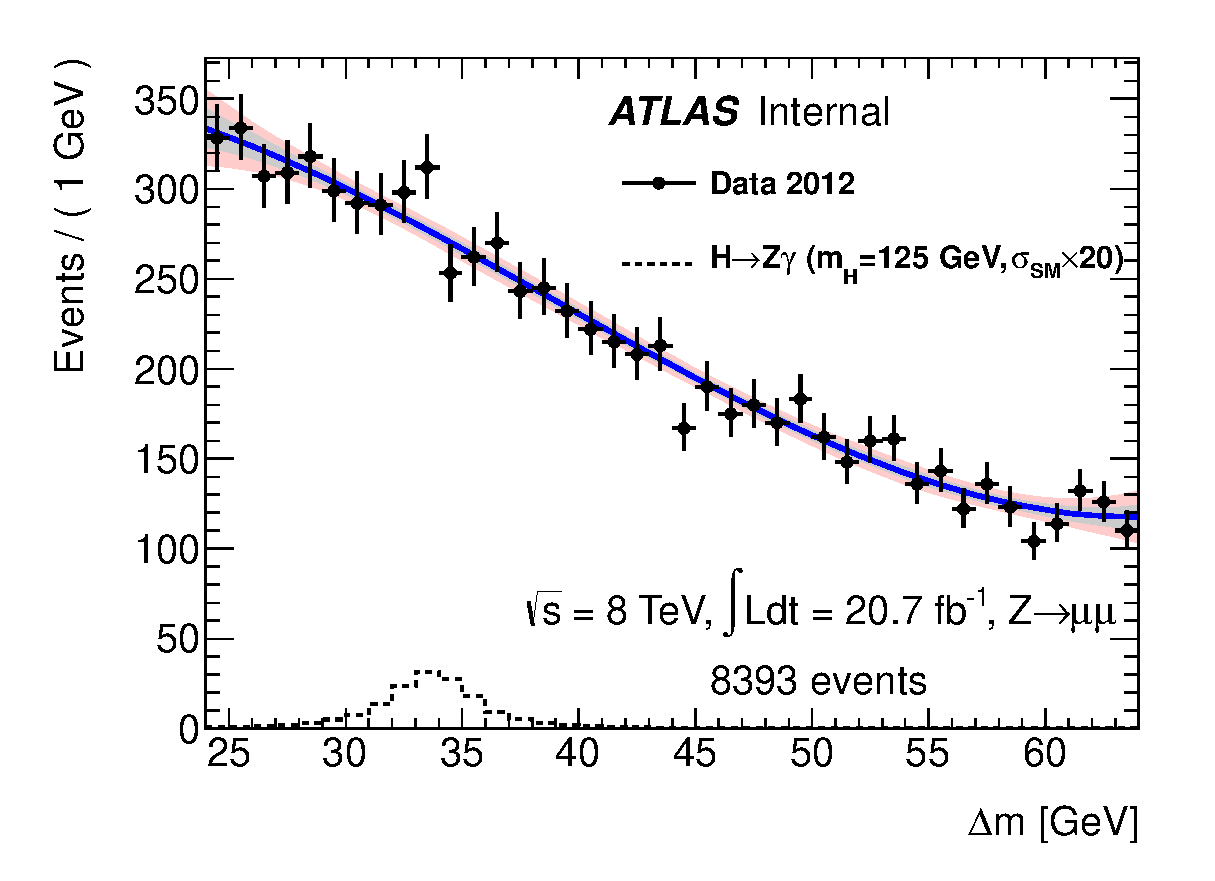
\includegraphics[width=0.49\columnwidth]{figures/bkgplots_mu_deltaM_fit_12_CB3_fiterr_internal_withsignal}
    \caption{Background-only fits to the distribution of 
      the mass difference $\Delta m$ of selected events in data,
      for $Z\to ee$ (left) and $Z\to\mu\mu$ (right), at $\sqrt{s}=7$ 
      TeV (top) or 8 TeV (bottom).
      For both 7 and 8 TeV, a third order polynomial is used for the fit.
      Dots correspond to data, the blue line is the fit result and the gray and light red
      bands are the 1$\sigma$ and 2$\sigma$ uncertainty 
      bands from the statistical uncertainties on the fitted 
      background model parameters.
      The dashed histograms correspond to the SM signal expectation,
      for a Higgs boson mass of 125 GeV, scaled by a factor 20 for clarity.
%%      The pulls of the data points with respect to the fit are also shown.
    }
    \label{fig:deltaM_data_bkgonly_fit}
  \end{center}
\end{figure}

\label{sec:background}

\section{Systematic Uncertainties}
\label{sec:sys}
A complete model of the signal and background distributions not only require
a description of the signal and background shapes observed in data, but also 
a quantification of the various uncertainties involved in the measurement.
The theoretical and experimental systematic uncertainties are summarized in
this section.

\subsection{Theoretical Uncertainties}
There are two sources of theoretical uncertainties on the production cross-section
of \HToZg events: the uncertainty related to the energy scales used for the
fixed-order calculation, and the uncertainty from the parton distribution functions
(PDFs) and the value of $\alphas$ used in the perturbative calculation. 

\begin{itemize}
\item \textbf{Scale Uncertainties:} 
In theoretical calculations, the value of observables are obtained using a 
perturbative expansion. This introduces an uncertainty due to missing higher order
corrections. In particular, the \HToZg signal cross-section is typically calculated
with leading-order (LO) matrix elements that can be corrected with higher-order
QCD (the production of a Higgs boson via gluon fusion is a QCD process) and 
electroweak corrections (Vector Boson Fusion production).

\item \textbf{Proton Structure Uncertainties:}
At the LHC Higgs bosons are produced using proton-proton collisions, so
an understanding of the \HToZg cross-section depends on the internal
parton structure of the proton. This internal proton structure cannot be
extracted from perturbation theory ($\alphas$ is large at the low binding
energies of the proton) and must be measured in the form of parton distribution
functions (PDFs). Consequently, the statistical and systematic uncertainties 
of these measurements must be propagated to any calculated cross-section.
\end{itemize}

The Higgs boson production
cross-sections and decay branching fractions as functions of the Higgs boson
mass are compiled, together with uncertainties, in Ref.~\cite{LHCHiggsCrossSectionWorkingGroup:2011ti}.
For each tested Higgs boson mass hypothesis the uncertainties from Ref.~\cite{LHCHiggsCrossSectionWorkingGroup:2011ti} are used.
\refT{tab:theory_uncertainties} summarizes uncertainties for a Higgs boson mass of
125 GeV. They depend only mildly on $m_H$, for $120 \GeV < m_H < 150 \GeV$,
with the exception of the relative uncertainty on the \HToZg branching fraction,
which varies between 9.4\% at 120 GeV and 6.2\% at 150 GeV.

Theoretical uncertainties on the background cross-sections do not affect the
results shown in the next section, because the background normalization and shape
are obtained through a fit to data.

\begin{table}[!htbp] 
  \renewcommand{\arraystretch}{1.3}
  \begin{center}
    \caption{Theoretical systematic uncertainties for the SM Higgs
      boson production cross section and branching fraction of the
      $H\to Z\gamma$ decay at $\sqrt{s} = 7$ and 8 TeV,
      for a Higgs boson mass of 125 GeV.}
    \label{tab:theory_uncertainties}
%\vspace{1mm}
    \begin{tabular}{l|cc|cc|cc|cc|cc|c}
      \hline\hline
$\sqrt{s}$ & \multicolumn{11}{c}{Systematic uncertainty (\%)}\\
%\hline
           & \multicolumn{2}{c}{$\sigma(gg\to H)$} & \multicolumn{2}{|c}{$\sigma$(VBF)} & \multicolumn{2}{|c}{$\sigma(WH)$} & \multicolumn{2}{|c}{$\sigma(ZH)$} & \multicolumn{2}{|c|}{$\sigma(t\bar tH)$} & $B(H\to Z\gamma)$ \\
         & scale & PDF & scale & PDF & scale & PDF & scale & PDF & scale & PDF & \\
\hline
7 TeV & $^{+7.1}_{-7.8}$  & $^{+7.6}_{-7.1}$  & {\small $\pm 0.3$} & $^{+2.5}_{-2.1}$ & $^{+0.2}_{-0.8}$ & {\small $\pm 3.5$} & $^{+1.4}_{-1.6}$ & {\small $\pm 3.5$} & $^{+3.3}_{-9.3}$  & {\small $\pm 8.5$} & $^{+9.0}_{-8.8}$ \\
8 TeV &$^{+7.3}_{-7.9}$  &$^{+7.5}_{-6.9}$   & {\small $\pm 0.2$} & $^{+2.6}_{-2.8}$ & $^{+0.1}_{-0.6}$ & {\small $\pm 3.4$} & $^{+1.5}_{-1.4}$ & {\small $\pm 3.5$} & $^{+3.9}_{-9.3}$  & {\small $\pm 7.8$} & $^{+9.0}_{-8.8}$ \\
  \hline\hline
    \end{tabular}
  \end{center}
\end{table}

\subsection{Experimental Uncertainties}
The following sources of experimental systematic uncertainties on the expected
signal yields have been considered:
\begin{itemize}
\item \textbf{Luminosity:}
The uncertainty on the integrated luminosity for the 2011 data is 1.8\% 
and $\pm 3.6\%$ in 2012 \cite{ATLAS:2012roa}.
%
\item \textbf{Acceptance of the kinematic requirements:}
The total acceptance of \HToZg events is defined as the ratio of the total number
of \HToZg events that pass all selections divided by the initial number of \HToZg
events. The uncertainties related to the acceptance of the selection criteria are
estimated using Monte Carlo simulations. This yields an uncertainty of 4\%.
%
\item \textbf{Photon identification efficiency:} 
Recall that to have reliable comparison between data and theory one uses Monte Carlo
simulation to generate events by computer randomly following a distribution predicted
by theory. However, there are areas where simulation can not reproduce data exactly
because there is no theory reproducing reality perfectly. In these areas on
need to bring Monte Carlo simulations to the level of data by hand. This is done
with the help of scale factors (SF) which are extracted from variables that are
easy to analyze. One such quantity is the photon identification efficiency scale
factor, which quantifies the discrepancy between data and MC when it comes to
identifying photons in the ATLAS detector. At $\rts = 7 \TeV$, the signal
yield is recomputing by varying the photon identification efficiency scale factors
within their uncertainties and the relative variation is considered as a systematic
uncertainty. At $\rts = 8 \TeV$ a conservative estimate of the uncertainty on the
photon identification efficiency obtained from a comparison between data-driven
measurements and the simulated efficiencies is used. This amounts to 2.5\% for
$\et < 40 \GeV$ and for unconverted photons with $\abseta > 1.81$ and to 1.5\%
otherwise. The resulting uncertainty on the \HToZg selection efficiency is below
3\%.
%
\item \textbf{Photon and electron calorimeter isolation requirements:}
The signal efficiency defined as $N_{\text{selected}}/N_{\text{truth}}$ 
is measured from simulated events. 
To estimate the systematic uncertainty due to the uncertainty
on the efficiency of the isolation criteria, the signal efficiency is recomputed
by shifting, in the simulation, the photon and electron calorimeter isolation
energies by the average difference observed between data and Monte Carlo for
photons and electrons, selected either in di-photon enriched events or
in a control sample of electrons from $Z \to ee$. These difference are of the
order of 100 MeV for the topological-cluster based isolation. The systematic
uncertainty on the signal efficiency range between 0.2\% and 0.4\%.
%
\item \textbf{Photon and electron energy scales:}
The energy of electromagnetic particles is measured by the electromagnetic 
calorimeter essentially through a measurement of the amount light produced by
the particle's interactions with the calorimeter's material. However, there
are a number of effects that spoil the accuracy of the conversion of light into
a particle's energy. The particles may punch through the calorimeter without leaving
their energy inside, or they hit parts of the device which are uninstrumented or
malfunctioning. Therefore, a correction to the energy measured in the 
electromagnetic calorimeter is applied known as an energy scale factor, which
rescales the measured energy to match the one the original particle had.

The uncertainty from the electromagnetic (photon and electron) energy
scales is assessed by varying the electromagnetic scale corrections (applied
to the data) within their uncertainties. The effects of the uncertainty fomr
the $Z \to ee$ calibration sample used to to extract the scale factors, of the
limited knowledge of the material, of the uncertainty on the pre-sampler energy 
scale and the low-$\pt$ scale factor uncertainties are evaluated. The total
uncertainty on the signal efficiency is around 0.2\% for events in which
the $Z$ boson candidate decays to muons and between 0.4\% and 1.2\% for
events in which the $Z$ boson candidate decays to electrons.
%
\item \textbf{Photon and electron energy resolution:}
The measurement of the electromagnetic energy only has a finite resolution.
The uncertainty from this electromagnetic energy resolution is estimated by
varying the resolution smearing corrections within its uncertainties and
observing the relative variation in the predicted signal yield. The estimated
uncertainty is smaller than 0.2\%.
%
\item \textbf{Electron trigger, reconstruction, and identification efficiency:}
The electron trigger, reconstruction, and identification efficiency uncertainties
are estimated by varying the efficiency scale factors applied to the simulation within
their uncertainties. The total uncertainty, for events in which the $Z$ boson
candidate decays to electrons, is around 3\%.
%
\item \textbf{Muon momentum scale and resolution:} 
The uncertainty of the efficiency of the $\pt > 10 \GeV$ cut (15 GeV for muons
tagged in the calorimeters) is estimated by varying the muon momentum
corrections in MC by their uncertainties. The effect is around 0.1\%.
%
\item \textbf{Muon trigger, reconstruction, and identification efficiency:}
The trigger, reconstruction, and identification muon efficiency uncertainties
are estimated by varying the efficiency scale factors within their uncertainties.
The total uncertainty, for events which $Z$ boson candidate decays to muons, is
below 1\%.
\end{itemize}
Other sources of uncertainties have been estimated by comparing the efficiencies
in data and Monte Carlo for control samples of leptons from $Z$ decays and found to
be negligible. The total relative uncertainty in the signal efficiency is around 5\%.

The following sources of experimental systematic uncertainties on the signal \dm
distribution have been considered:
\begin{itemize}
\item \textbf{Photon and energy scales:}
The signal \dm distribution is recomputed after varying the electromagnetic
energy scale corrections within their uncertainties, and the shift of the
peak position (0.2 GeV) is considered the systematic uncertainty.
%
\item \textbf{Photon and electron energy resolution:}
The signal \dm distribution is recomputed after varying the electromagnetic
smearing corrections within their uncertainties, and the relative variation of
its width is taken as a systematic uncertainty. It amounts to 2-4\% for events
in which the $Z$ boson candidate decays to muons and to 5\% for events in which the 
$Z$ boson candidate decays to electrons.
%
\item \textbf{Muon momentum scale:}
The signal \dm distribution is recomputed after varying the muon momentum scale
within its uncertainties, and the shift of the peak position is considered
as a systematic uncertainty. This uncertainty is found to be negligible.
%
\item \textbf{Muon momentum resolution:}
The signal \dm distribution is recomputed after varying the muon momentum smearing
corrections within their uncertainties, and the relative variation of its
width (0-1.5\%) is taken as a systematic uncertainty.
\end{itemize}

The list of the main sources of systematic uncertainties and their contributions
to the \HToZg expected signal yields and parameters of the signal \dm distributions
are listed in Table~\ref{tab:zg_syst_125_8_7tev} for $m_H = 125 \GeV$ and
$\rts = 8$ (7) TeV. The systematic uncertainties are profiled in the final
maximum likelihood fit to the data, as described in \refS{subsec:nuisance}. All
systematic uncertainties, except that on the luminosity, are treated as
correlated between $\rts = 7 \TeV$ and the $\rts = 8 \TeV$ analyses.

\begin{table}[!htbp]
\centering
\caption{Summary of the systematic uncertainties on the signal yield and
  invariant mass distribution for $m_H = 125$ GeV, at $\sqrt{s}=8 (7)$ TeV.}
  \label{tab:zg_syst_125_8_7tev} 
\small
 \begin{tabular}{cccc}
       \hline
       \hline
       \textbf{Systematic Uncertainty }           & $H \rightarrow Z(ee) \gamma$(\%)   & $H \rightarrow Z(\mu\mu) \gamma$(\%) \\
       \hline
       \textbf{Signal Yield}                      &                                    &                                      \\ 
       \hline
       \multicolumn{1}{l}{Luminosity}                                 & 3.6 (1.8)                        & 3.6 (1.8)          \\
       \multicolumn{1}{l}{Trigger efficiency}                         & 0.4 (0.2)                        & 0.8 (0.7)          \\
       \multicolumn{1}{l}{Acceptance of kinematic selection}          & 4.0 (4.0)                        & 4.0 (4.0)          \\
       \multicolumn{1}{l}{$\gamma$ identification efficiency}         & 2.9 (2.9)                        & 2.9 (2.9)          \\  
       \multicolumn{1}{l}{electron reconstruction and identification efficiency} & 2.7 (3.0)             &                    \\  
       \multicolumn{1}{l}{$\mu$ reconstruction and identification efficiency}    &                       & 0.6 (0.7)          \\  
       \multicolumn{1}{l}{$e/\gamma$ energy scale}                    & 1.4 (0.3)                        & 0.3 (0.2)          \\
%%       \multicolumn{1}{r}{Method uncertainty ($Z\to ee$)} & \multicolumn{1}{r}{1.4 (0.2)}   & \multicolumn{1}{r}{0.2 (0.1)} \\
%%       \multicolumn{1}{r}{Material uncertainty}   & \multicolumn{1}{r}{0.1 (0.1)}    & \multicolumn{1}{r}{0.2 (0.1)}        \\
%%       \multicolumn{1}{r}{Presampler energy scale}& \multicolumn{1}{r}{0.0 (0.1)}    & \multicolumn{1}{r}{0.0 (0.0)}        \\
%%       \multicolumn{1}{r}{Low pt}                 & \multicolumn{1}{r}{0.2 (0.2)}    & \multicolumn{1}{r}{0.2 (0.1)}        \\
       \multicolumn{1}{l}{$e/\gamma$ isolation}                       & 0.4 (0.3)                        & 0.4 (0.2)          \\  
       \multicolumn{1}{l}{$e/\gamma$ energy resolution}               & 0.2 (0.2)                        & 0.0 (0.0)          \\
       \multicolumn{1}{l}{$\mu$ momentum scale}                       &                                  & 0.1 (0.1)          \\  
       \multicolumn{1}{l}{$\mu$ momentum resolution}                  &                                  & 0.0 (0.1)          \\
       \hline
       \textbf{Signal $\Delta m$ resolution}      &                                    &                                      \\  
       \hline 
       \multicolumn{1}{l}{$e/\gamma$ energy resolution}               & 5.0 (5.0)                        & 2.4 (2.4)          \\ 
       \multicolumn{1}{l}{$\mu$ momentum resolution}                  &                                  & 0.0 (1.5)          \\
       \hline
       \textbf{Signal $\Delta m$ peak position} \\
       \hline
       \multicolumn{1}{l}{$e/\gamma$ energy scale}                    & 0.2 (0.2) GeV                    & 0.2 (0.2) GeV    \\
       \multicolumn{1}{l}{$\mu$ momentum scale}                       &                                  & negligible         \\
       \hline
       \hline
 \end{tabular}
\end{table}

\label{sec:sys}

\section{Results}
\label{sec:results}

\subsection{Statistical method for the evaluation of limits and $p$-values}
\label{subsec:statintro}
Evidence for \HToZg production at the LHC would be an excess of Higgs bosons 
in the \dm or \mllg invariant mass distributions over the background of known
Standard Model processes. As such, likelihood-based statistical tests are used to
interpreted the selected data samples in terms of the SM background plus the 
contribution of a Standard Model Higgs boson decaying to $Z\gamma$.
The results are expressed in terms of a ``signal-strength" parameter 
$\mu$, which is defined as the ratio
\[
    \mu = \frac{N_{\text{signal}}}{N_{\text{signal}}^{\text{SM}}}
\]
of the measured number of signal events to the value expected by the
Standard Model. For a Standard Model Higgs boson decaying to $Z\gamma$,
the value of $\mu$ should be consistent with unity within statistical uncertainties.

First, in order to quantify the significance of a possible observation,
a hypothesis test is performed to evaluate the
compatibility between the data and the null hypothesis, which assumes
that the selected data contains only background events. If the hypothesis
test shows no presence of any significant excess in the data, 
a limit on the ratio of the \HToZg cross-section over the Standard Model 
expectation is set. These results are quoted for a possible Higgs boson mass 
between 120 and 150 GeV.

\subsubsection{$p$-value calculation}
Any statistical hypothesis test begins by defining two competing hypothesis:
the null and alternate hypothesis. Here the null hypothesis corresponds to the
hypothesis that the data contains only Standard Model background processes 
($\mu = 0$), i.e. the background-only (B-only) hypothesis. 
In contrast, the alternate hypothesis is the conjecture that a Standard Model
Higgs boson is contained in the data ($\mu = 1$). This hypothesis is also known
as the signal plus background (S+B) hypothesis. The compatibility of the
data with the background-only hypothesis is quantified by the $p_0$ or $p$-value
of the data, which gives the probability for a dataset generated in the
B-only hypothesis to be in the same or worse agreement with that hypothesis.
Only upward deviations from the B-only hypothesis, which would correspond to
a positive signal strength, are considered. Large \pzero therefore correspond
to datasets that agree well with the B-only hypothesis, while small \pzero can
be interpreted as a suggestion of a significant positive signal.

In order to investigate the measure of agreement between the observed data
and a given hypothesis, one constructs a function of the data
called a test statistic. The test statistic is designed to reduce a large
quantity of data points to a single value whose distribution can be used to
distinguish the null from the alternative hypothesis through a 
hypothesis test. Following the ATLAS recommendations~\cite{ATLAS_stat_recommendations}
, the \pzero is computed from the $q_0$ test statistic, defined as
\[
    q_0 =
    \begin{cases}
        -2\ln{\frac{L(0,\hat{\hat\theta}(0))}{L(\hat\mu,\hat\theta)}} & \hat\mu \ge 0 \\
        +2\ln{\frac{L(0,\hat{\hat\theta}(0))}{L(\hat\mu,\hat\theta)}} & \hat\mu < 0
    \end{cases}
\]
where $L$ is the likelihood function described in \refS{subsec:likelihood},
$\hat \mu$ and $\hat \theta$ are the best-fit values for $\mu$ and $\theta$
with all parameters floating, and $\hat{\hat\theta}(0)$ is the best-fit value of
$\theta$ in the B-only ($\mu=0$) hypothesis. 

In the expression for $\hat\mu > 0$, 
the numerator corresponds to the best value of the likelihood computed in the
B-only hypothesis, while the denominator corresponds to the best value in the
S+B hypothesis including both signal and background. Therefore, for datasets 
compatible with the B-only hypothesis, both should be of similar magnitude and
$q_0$ will be small. Conversely, in the presence of a signal the denominator
(S+B hypothesis) should be much larger than the numerator (B-only hypothesis),
yielding a large value for $q_0$. These observations lead to the following
definition for the $p$-value of the null hypothesis:
\[
    p_0 = \int_{q_{0,\text{obs.}}}^{\infty} f(q_0|0,m_H,\hat{\hat\theta}(0))\,dq_0
\]
where $f$ is the distribution of the test statistic. An illustration of this 
calculation is presented in \refF{fig:pvalue}. This definition is equivalent
to saying that the $p$-value gives the probability for a dataset generated in the
null hypothesis to be in the same or worse agreement with that hypothesis since
large values of $q_0$ correspond to the data being incompatible with the B-only
hypothesis. In this scheme, small $p_0$ occurs only for $q_0 > 0$, which happens
only for $\hat\mu \ge 0$. This corresponds to the one-sided prescription mentioned
above, where only positive (``physical") values of the signal are considered. 
Negative fluctuations of the  signal are assigned $p_0$ values in the interval
$[0.5,1]$, with values close to 0.5 corresponding to small negative fluctuations,
and values close to 1 for large negative fluctuations.

\begin{figure}[htbp]
    \centering
    \includegraphics[scale=0.4, angle=0]{./figures/pvalue}
    \caption{Illustration of the relation between the $p$-value obtained from an
    observed value of the test statistic $t_{\mu}$ (this corresponds to $q_0$ in
    the discussion presented in this paper). This figure is taken from 
    \cite{Cowan:2010js}.}
    \label{fig:pvalue}
\end{figure}

It should be noted that in the asymptotic regime, which is usually a good
approximation for the models studied here, $p_0$ values can be directly computed
from the $q_0$ values using a closed form asymptotic formulae \cite{Cowan:2010js}.
Alternatively, the \pzero can be computed by sampling the distribution of $q_0$
in the B-only hypothesis using pseudo-experiments. Unless otherwise stated, 
asymptotic formulae will be used in the results presented here. In the following,
we present both \emph{observed} $p_0$ results, computed using real data, and
\emph{expected} $p_0$, which are computed from an Asimov dataset\footnote{
An Asimov dataset is defined such that when one uses it to evaluate the 
estimators for all parameters, one obtains the true parameter values.}
in the $\mu = 1$ hypothesis.

\subsubsection{Limit-setting}
If one finds that the data is compatible with the B-only hypothesis, then this
is an indication that there is not a significant excess of signal in the data
(it does not rule out the S+B hypothesis). The question that is then asked is
how large the signal's production cross-section can be before one would expect
to measure signal events with the amount of data collected so far. 
If the upper limit on the signal strength $\mu$ lies
below unity indicating that less Higg's bosons are produced then predicted by 
the Standard Model, then that is an indication that the S+B hypothesis is incorrect.

Upper limits on the signal strength are set using a modified frequentest ($CL_s$)
method \cite{cls}, using a $CL_{s+B}$ based on the \qmu test statistic,
as recommended by the ATLAS Collaboration \cite{ATLAS_stat_recommendations}. 
The test statistic is computed as
\[
    \tilde q_{\mu} =
    \begin{cases}
        -2\ln{\frac{L(\mu,\hat{\hat\theta}(\mu))}{L(\hat\mu,\hat\theta)}} & 0 \le \hat\mu \le \mu \\
        0 & \hat\mu > \mu \\
        -2\ln{\frac{L(0,\hat{\hat\theta}(0))}{L(\hat\mu,\hat\theta)}} & \hat\mu < 0
    \end{cases}
\]
where $L$ is the likelihood function described in \refS{subsec:likelihood},
$\hat\mu$ and $\hat\theta$ are the best-fit values for $\mu$ and $\theta$ with
all parameters floating, and $\hat{\hat\theta}(\mu)$ is the best-fit value for
$\theta$ for a fixed value of $\mu$. The statistic estimates the compatibility 
of the data with the $\mu$ hypothesis using the ratio of likelihoods for the case
of floating $\mu$ (denominator), and the case where it is fixed at the hypothesis
value (numerator). As for the case of $q_0$, a one-sided prescription is used,
assigning $\qmu = 0$ if the fitted value $\hat\mu$ is above the hypothesis.
Finally, if $\hat\mu < 0$, the case $\mu=0$ is used instead to avoid technical
issues with negative p.d.fs.

The $CL_{s+b}$ $p$-value is defined as:
\[
    p_{s+b} = \int_{\tilde q_{\mu,\text{obs.}}}^{\infty} f(\qmu|\mu,m_H,\hat{\hat\theta}(\mu))\,d\qmu
\]
and the $CL_s$ $p$-value is
\[
    p_{\mu} = \frac{p_{s+b}}{p_b}
\]
where
\[
    p_{b} = 1 - \int_{\tilde q_{\mu,\text{obs.}}}^{\infty} f(\qmu|0,m_H,\hat{\hat\theta}(0))\,d\qmu.
\]
is the $CL_b$ $p$-value. A description of the various $p$-values used in the $CL_s$
exclusion method is presented in \refF{fig:cls}.
The value of $p_{\mu}$ and of the corresponding $CL_s$ exclusion are obtained
using either asymptotic formulae \cite{Cowan:2010js} or pseudo-data generation.
Limits at a 95\% confidence level on the value of the signal strength $\mu$ are
then computed by scanning values of the $\mu$ hypothesis, computing the $CL_s$
exclusions and identifying $\mu_{\text{up}}$ for which this value equals 0.05.

\begin{figure}[htbp]
    \centering
    \includegraphics[scale=0.4, angle=0]{./figures/CLs}
    \caption{The distribution of the statistic $q = -2\ln(L_{s+b}/L_b)$ under the 
    hypotheses $\mu=0$ and $\mu=1$. The $CL_s$ exclusion is defined as the ratio
    between $p_{s+b}$ and $p_{b}$. This figure was taken from \cite{Cowan:2010js}.}
    \label{fig:cls}
\end{figure}

We will present both observed limits, computed using real data, and expected limits
computed using an Asimov dataset generated in the $\mu=0$ hypothesis.

\subsection{Likelihood}
\label{subsec:likelihood}
When performing a hypothesis test on a set of data, one needs a function that 
quantifies the probability of those observations given a set of parameters
set by the hypothesis. In particle physics experiments at ATLAS, a discovery
of a new particle typically proceeds through an analysis of 
invariant mass distributions, such as \dm or \mllg, whose shape and normalization 
are determined by the B-only and S+B hypotheses. 
Given an observed invariant mass distribution one wants
to quantify the probability of observing this distribution given the predictions of 
the Standard Model. The answer to this question is obtained using an 
unbinned maximum likelihood (ML) depending on a single observable $x$, which
is either the invariant mass \mllg or the invariant mass difference \dm. As
mentioned in \refS{subsec:statintro}, we consider a single parameter of interest
in the model, the signal strength $\mu$. In addition to $\mu$, the likelihood
depends on several additional \emph{nuisance} parameters, like the number of
background events or the parameters characterizing the probability distribution
functions of the variable $x$ for signal and background events. For some of
these nuisance parameters, additional prior information may be available, for 
instance from theoretical calculations or from measurements performed in control
samples; in that case, the corresponding probability density function for those
parameters is incorporated into the full likelihood function as described in
\refS{subsec:nuisance}.

The data is split into four discrete, orthogonal categories: two categories,
depending on the flavor of leptons produced by the $Z$ decays ($\ell = e, \mu$),
for each of the two center-or-mass energies (7 and 8 TeV) at which the data was
collected. In order to extract the results, a simultaneous unbinned maximum
likelihood fit to the distribution of $c$ in all the categories was performed.
The full likelihood is written as:
\[
    L\left(\mu,\theta=\bigcup_{c=1}^{n_{cat}}\theta_c|x=\bigcup_{c=1}^{n_{cat}} 
    x_c\right) = 
    \prod_{c=1}^{n_{cat}} L_c(\mu,\theta_c|x_c)
\]
where $n_{cat}=4$ is the number of categories, $\theta_c$ are the nuisance
parameters used to describe the model in category $c$ and $x_c$ is the set of
experimental measurements of the observable $x$ in the same category. $L_c$
is the likelihood in category $c$:
\[
    L_c(\mu,\theta_c|x_c) = \frac{({N'}_c)^{N_c} e^{-{N'}_c}}{N_c !} \prod_{k=1}^{N_c}
    \mathcal{L}_c(x_k|\mu,\theta_c) = 
    \text{Pois}(N_c|{N'}_c) \prod_{k=1}^{N_c} \mathcal{L}_c(x_k|\mu,\theta_c) 
\]
where $N_c$ is the number of selected events, $x_k$ is the value of $x$ measured
in event $k$, $N_{\text{signal},c}$ and $N_{\text{bkg},c}$ are the number of
signal and background events, and ${N'}_c = (N_{\text{signal},c} + N_{\text{bkg},c})$
where each quantity refers to category $c$. The term outside the product is a
Poisson probability factor for ${N'}_c$, which when maximizing the likelihood with
respect to ${N'}_c$ will force the maximum likelihood (ML) estimates of the signal
and background yields to satisfy $\hat N_{\text{signal},c} + \hat N_{\text{bkg},c} =
N_c$. $\mathcal{L}_c(x_k|\mu,\theta_c)$ is the per-event likelihood, i.e. the 
probability, for category $C$, to measure the value $x=x_k$ if the values
of the strength parameter and the nuisance parameters are $\mu$ and $\theta_c$.
Except where otherwise stated, it is taken to be of the form
\[
    \mathcal{L}_c(x|\mu,\theta_c) = \frac{N_{\text{signal},c}(\mu,\theta_c^{\text{norm}})}{N_{\text{signal},c} + N_{\text{bkg},c}}\, f_{\text{signal},c}(x|\theta_c^{\text{shape}}) 
    + \frac{N_{\text{bkg},c}}{N_{\text{signal},c} + N_{\text{bkg},c}}\, f_{\text{bkg},c}(x|\theta_c^{\text{bkg}})
\]
where $f_{\text{signal},c}$ and $f_{\text{bkg},c}$ are the signal and background
probability distribution functions for category $c$, and $\theta_c^{\text{norm}}$,
$\theta_c^{\text{shape}}$, and $\theta_c^{\text{bkg}}$ are the nuisance parameters
used in the description of the expected signal yield, the signal p.d.f., and the
background p.d.f. respectively. The full set of nuisance parameters for each category
$c$ can thus be identified as 
$\theta_c = \theta_c^{\text{norm}} \cup \theta_c^{\text{shape}} \cup 
\theta_c^{\text{bkg}} \cup N_{\text{bkg},c}$. The treatment of systematic 
uncertainties on this physics model are described in \refS{subsec:nuisance}.


\subsection{Treatment of systematic uncertainties}
\label{subsec:nuisance}
In order to incorporate systematic uncertainties into the calculation
of $p$-values and confidence intervals described in the previous section,
an assignment of p.d.f.s to relative uncertainties in the measurement
must be carried out.
In particular, a nuisance parameter $\theta$ is associated with each source
of uncertainty, so that that the signal yields or parameters of the model
becomes functions of $\theta$. One then incorporates a ``penalty" or ``constraint"
term into the final calculation, which exploits the best estimate that we have
of each systematic uncertainty. The nuisance parameters are then fitted (``profiled")
to the data, together with the parameters of interest, when minimizing $-\log L$.
 
In practice, the systematic uncertainties follow either a Gaussian or Log-normal 
form, which depends on the source of the uncertainty. 
If the systematic uncertainty affects the expected signal yield,
the Log-normal form is used to avoid the negative tails. While if it represents
a migration between categories (lepton flavor in the final state), the Gaussian
form is used. For a systematic uncertainty $\sigma$ for which a Gaussian constraint 
is assumed, a nuisance parameter $\theta$ is added that samples from a normal 
distribution $G$ and the constraint term is of the form
\[
    (1 + \sigma\theta),
\]
i.e. the product $A_0 \, G(\theta)\,(1+\sigma\theta)$ is a p.d.f for an observable 
$A$ with mean equal to some nominal value $A_0$ and width equal to the systematic
uncertainty $\sigma$. Similarly, for a systematic uncertainty $\sigma$ for which
a Log-normal constraint is assumed, a nuisance parameter $\theta$ is added
that samples from a normal distribution and the constraint term is of the form
\[
    e^{\sqrt{\log(1+\sigma^2)}\theta}
\]
i.e. the logarithm of the quantity $\exp({\sqrt{\log(1+\sigma^2)}\theta)}$ has
a Gaussian p.d.f. with mean 0 and width equal to one. In the cases where the
uncertainty is asymmetric, a bifurcated Gaussian is actually used as a
constraint instead of a Gaussian. In this case the $\sigma$ is taken to be the
negative uncertainty, and the ratio of positive to negative uncertainties is used
as the right width of the bifurcated Gaussian. The left width is taken to be unity.
As in other ATLAS Higgs searches, all systematic uncertainties except the 
luminosity ones are considered fully correlated between 2011 and 2012 datasets.
 
\subsection{Comparison to the background-only hypothesis and exclusion limits} 
The expected and observed \pzero values are shown in \refF{fig:ExpectedP0_1}
as a function of the Higgs boson mass. Using the full 2011 and 2012 ATLAS data,
corresponding to 4.6 \ifb of $pp$ collisions at $\rts = 7 \TeV$ and 20.7 \ifb
of $pp$ collisions at $\rts=8\TeV$, the expected \pzero ranges between 0.40
and 0.46 for $120 < m_H < 150 \GeV$, corresponding to a significance of 0.25$\sigma$.
The observed \pzero distribution is compatible with the data being composed of
background only. The smallest \pzero (0.042) corresponds to a significance of
$1.61\sigma$, occurs for a mass of 141 GeV. The expected \pzero at $m_H = 125 \GeV$
is 0.443, corresponding to a significance of $0.14\sigma$, while the observed one
is 0.188 (0.89$\sigma$).

\begin{figure}[!htbp]
\centering
    {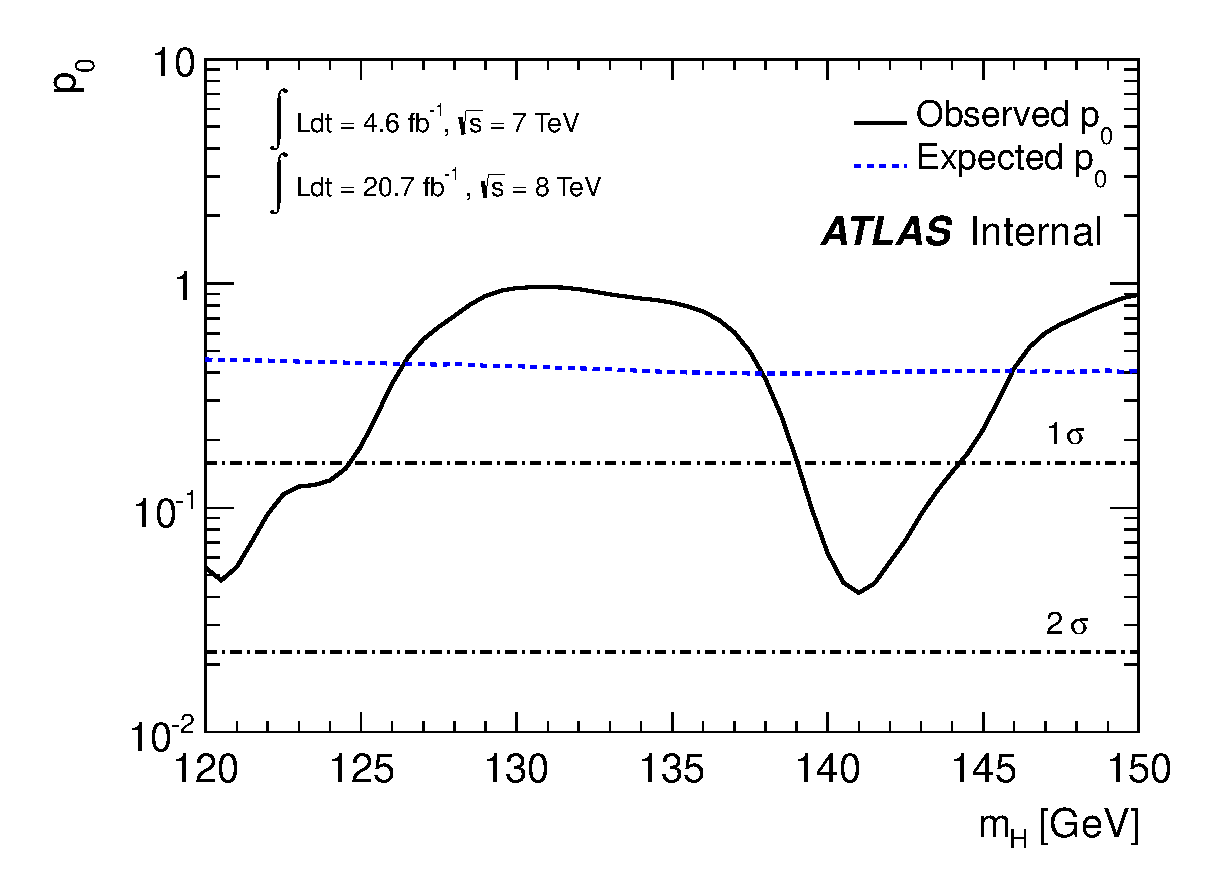
\includegraphics[totalheight=9cm,angle=0]{figures/plot_p0}}
    \caption{Expected (dashed blue line) and observed 
      (solid black line) $p_0$ (compatibility of
      the data with the background-only hypothesis) as a function
      of the Higgs boson mass, using \lumiseventev~\ifb\ of $pp$
      collisions at $\sqrt{s}=7$~TeV and \lumieighttev~\ifb\ of $pp$
      collisions at $\sqrt{s}=8$~TeV.}
    \label{fig:ExpectedP0_1}
\end{figure}

Subsequently, upper limits on the production cross-section of \HToZg are set.
Both observed limits, computed using real data, and expected limits, computed
Asimov dataset generated with the $\mu=0$ hypothesis are shown in 
\refF{fig:ExpectedExclusion_1}. The expected 95\% $CL_s$ limit ranges between
7.3 and 22 and the observed one varies between 5.4 and 37 for a Higgs boson
mass between 120 and 150 GeV. In particular, for a mass of 125 GeV, consistent
with the mass of the recently discovered Higgs-like boson, the expect and observed
limits are equal to 13.5 and 18.2 times the Standard Model, respectively. The
results are dominated by the statistical uncertainties.

\begin{figure}[!htbp]
\centering
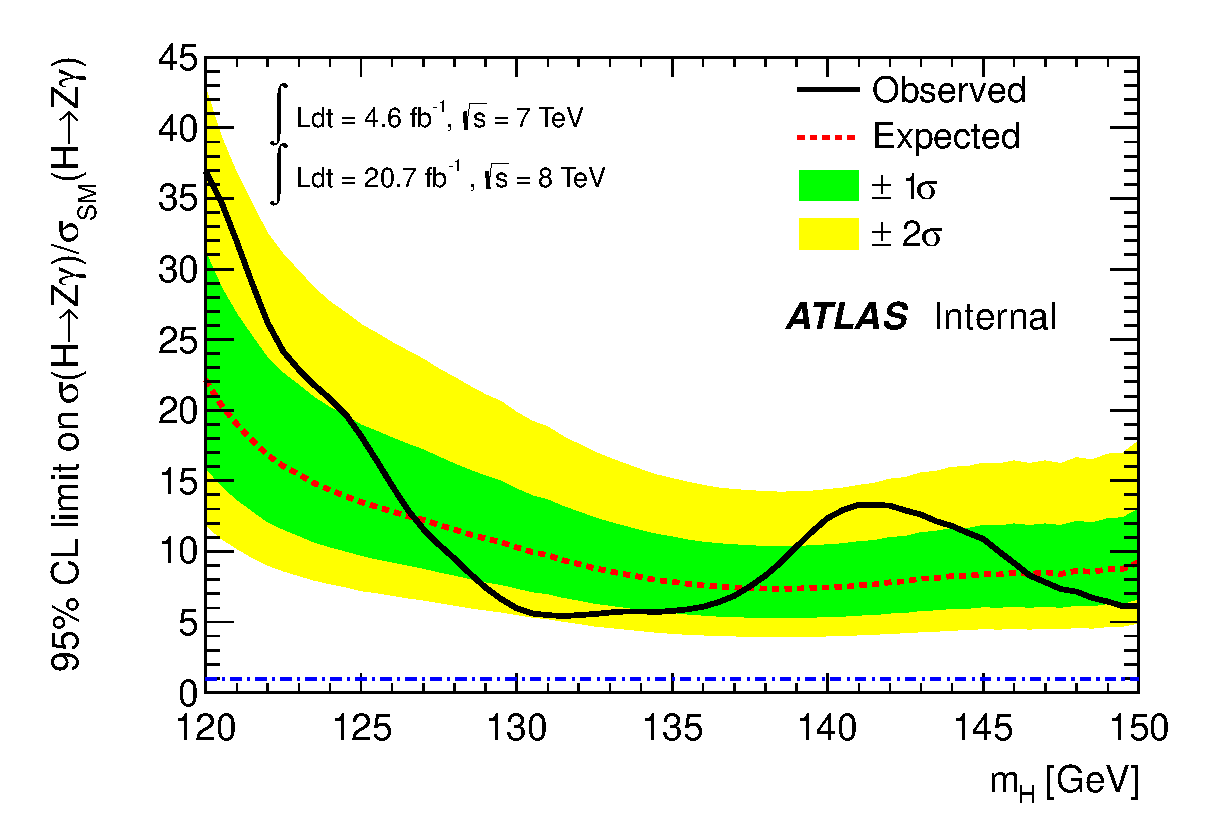
\includegraphics[totalheight=9cm,angle=0]{figures/plot_smooth_cls}
\caption{Observed 95\% $CL$ limits (solid black line) 
  on the production cross section of a SM Higgs boson 
  decaying to $Z\gamma$, as a function of the Higgs boson 
  mass, using \lumiseventev~\ifb\ of $pp$
  collisions at $\sqrt{s}=7$~TeV and \lumieighttev~\ifb\ of $pp$
  collisions at $\sqrt{s}=8$~TeV.
  The median expected 95\% $CL$ exclusion limits (dashed red line)
  are also shown. The green and yellow bands correspond to the $\pm 1\sigma$ 
  and $\pm2\sigma$ intervals.
}
\label{fig:ExpectedExclusion_1}
\end{figure}

\label{sec:results}

\bibliographystyle{atlasnote}
\bibliography{biblio}

\end{document}
